\documentclass[12pt, draftcls, onecolumn]{IEEEtran}

% Packages
\usepackage{bm}
\usepackage{url}
\usepackage{bbm}
\usepackage{cite}
\usepackage{array}
\usepackage{ifthen}
\usepackage{xspace}
\usepackage{dsfont}
\usepackage{siunitx}
\usepackage{amsmath}
\usepackage{amssymb}
\usepackage{multicol}
\usepackage{amsfonts}
\usepackage{mathrsfs}
\usepackage{booktabs}
\usepackage{graphicx}
\usepackage{caption}
\usepackage{setspace}
\usepackage{hyperref}
\usepackage{makecell}
\usepackage{footnote}
\usepackage{verbatim}
\usepackage{algorithm}
\usepackage{subcaption}
\usepackage{glossaries}
\usepackage{soul,xcolor}
\usepackage[T1]{fontenc}
\usepackage{algpseudocode}
\usepackage{algcompatible}
\usepackage[normalem]{ulem}
\usepackage{multirow, enumitem}

% Setting up packages
\captionsetup{font=footnotesize}
\setlength{\textfloatsep}{1.5pt}
\sisetup{detect-all,range-phrase=--,range-units=single,group-separator={,}}

% Initializing new commands
\newcommand{\sst}[1]{\st{#1}}
\newcommand{\tot}{\mathrm{tot}}
\newcommand{\tfrm}{T_{\mathrm{fr}}}
\newcommand{\beam}[1]{\mathcal B_{#1}}
\newcommand{\add}[1]{\textcolor{red}{#1}}
\newcommand{\size}[1]{\left | #1 \right|}
\newcommand{\bk}[1]{\textcolor{blue}{[BK: #1]}}
\newcommand{\yz}[1]{\textcolor{blue}{[YZ: #1]}}
\newcommand{\ca}[1]{\textcolor{magenta}{[CA: #1]}}
\newcommand{\nm}[1]{\textcolor{magenta}{[NM: #1]}}
\newcommand{\jvk}[1]{\textcolor{magenta}{[JVK: #1]}}
\newcommand{\djl}[1]{\textcolor{magenta}{[DJL: #1]}}
\newcommand{\beambs}[1]{\mathcal B_{{\mathrm t},#1}}
\newcommand{\beamue}[1]{\mathcal B_{{\mathrm r},#1}}
\newcommand{\diag}[1]{\mathrm{diag}\left(#1 \right)}
\newcommand{\numberthis}{\addtocounter{equation}{1}\tag{\theequation}}
\newcommand\mst[2][red]{\setbox0=\hbox{$#2$}\rlap{\raisebox{.45\ht0}{\textcolor{#1}{\rule{\wd0}{2pt}}}}#2}

% Redefining commands
\renewcommand\theadalign{c}
\renewcommand{\tabcolsep}{1pt}
\renewcommand\theadfont{\bfseries}
\renewcommand\cellgape{\Gape[2pt]}
\renewcommand\theadgape{\Gape[2pt]}

% Title, Authors, and Footnotes
\title{Multipath Clustering and Channel Modeling at \SI{28}{\giga\hertz} via Beam-Steered V$2$X Measurements}
\author{Bharath Keshavamurthy\IEEEauthorrefmark{1}, Yaguang Zhang\IEEEauthorrefmark{2}, Christopher R. Anderson\IEEEauthorrefmark{3},\\\ \ \ \ Nicol\`{o} Michelusi\IEEEauthorrefmark{1}, David J. Love\IEEEauthorrefmark{2}, and James V. Krogmeier\IEEEauthorrefmark{2}
\thanks{Preliminary version accepted at IEEE ICC $2023$~\cite{ICC}. Source code available on \href{https://github.com/bharathkeshavamurthy/SPAVE-28G.git}{GitHub}\cite{SPAVE-28G-Software}. Datasets available on \href{https://doi.org/10.5281/zenodo.7178597}{Zenodo}\cite{SPAVE-28G-Dataset}.}
\thanks{\IEEEauthorrefmark{1}ECEE, Arizona State University. \IEEEauthorrefmark{2}ECE, Purdue University. \IEEEauthorrefmark{3}EEE, United States Naval Academy.}
\thanks{This research has been funded by NSF under grants CNS-$1642982$ and CNS-$2129615$.}
\vspace{-8mm}
}

% Content begins
\begin{document}
\bstctlcite{IEEEexample:BSTcontrol}

\maketitle
\thispagestyle{plain}
\pagestyle{plain}
\setulcolor{red}
\setul{red}{2pt}
\setstcolor{red}
\vspace{-8mm}

% Abstract
\begin{abstract}
This work details the design of a fully-autonomous mechanical beam-steering platform, equipped with a sliding-correlator channel sounder, for \SI{28}{\giga\hertz} V2X propagation modeling on the NSF POWDER testbed. The compiled datasets constitute geo-positioning logs, beam-alignment specifics, and signal propagation measurements, along unplanned vehicular routes in urban and suburban radio environments. Leveraging design encapsulation and uninhibited rotational mobility of this beam-alignment platform enables continuous series of measurements, a unique yet critical necessity for millimeter wave channel modeling in vehicular networks. The calibrated and processed datasets facilitate crucial propagation analyses necessary for the efficient design and deployment of next-generation V$2$I/V$2$V networks. First, this paper studies the pathloss behavior of \SI{28}{\giga\hertz} signals along various routes onsite, and empirically evaluates the correctness of popular outdoor micro- and macro-cellular pathloss standards -- namely, $3$GPP TR$38.901$, ITU-R M$.2135$, METIS, and mmMAGIC. Next, assessing the spatial autocorrelation coefficient under Tx-Rx distance, alignment accuracy, and relative velocity variations, delivers novel insights on signal decoherence characteristics. Furthermore, power delay angular profiles allow the analysis of temporal and spatial dispersion attributes along OLoS and NLoS links, while power delay Doppler profiles permit Doppler shift and Doppler spectra investigations in highly-mobile scenarios. Employing a custom implementation of the SAGE algorithm, multipath clustering analyses -- centered around the Kolmogorov-Smirnov statistic -- facilitate empirical validations of the Saleh-Valenzuela, Quasi-Deterministic, Device-to-Device, and stochastic channel models vis-\`{a}-vis cluster arrival and decay characteristics, RMS delay- and direction-spreads, and shadow fading distributions. Lastly, in addition to the geometry-induced losses highlighted above, this paper examines the fast-fading properties of the obstructed signal, i.e., average fade depth and duration, under dynamic blockages in V2X settings.
\end{abstract}
\vspace{-4mm}

% Index terms
\begin{IEEEkeywords}
    Millimeter wave, V2X, Beam-alignment, Pathloss, Multipath clustering, Doppler spectrum
\end{IEEEkeywords}
\vspace{-4mm}

% Introduction, Literature survey, and Novelties
\section{Introduction}\label{S1}
With the widespread adoption and recent acceleration in the deployment of $5$G networks, primarily leveraging the mid-band spectrum (C-band: \SIrange{4}{8}{\giga\hertz}), service providers have now shifted their spectrum procurement focus to the millimeter wave bands (mmWave: \SIrange{30}{300}{\giga\hertz}) for next-generation radio access technologies, viz., $5$G$+$ and $6$G~\cite{mmWaveSurvey, Commercial, 5GBSurvey, 6GSurvey}, with the long-term vision of providing significant enhancements in user experience vis-\`{a}-vis data rates and latencies. Concertedly, academic research and industrial R\&D activities on mmWave propagation modeling and system design have gained a renewed emphasis -- specifically in relation to vehicular networks~\cite{VehicularBeamSelection, CVBeamAlignmentV2X}, non-terrestrial communications~\cite{mmWaveRuralNTNOpportunities, UAVBeamTracking}, and A.I.-native PHYs~\cite{6GAINative, OTAGANs}. However, the promise of ultra-reliable low-latency communications envisioned by mmWave networks involves numerous challenges, the most demanding one being the poor propagation characteristics of these extremely high frequency signals. In particular, mmWave signals suffer from increased atmospheric attenuation due to their relatively high free-space pathloss, in addition to absorption and scattering effects \cite{Rappaport}; significant slow-fading (shadowing) consequences due to obstacles \cite{SuburbanGeometryJournal}; exacerbated fading behavior brought on by multipath propagation due to diffuse reflections off surfaces, and diffractions by foliage and building-edges \cite{Outdoor28G}; and finally, unavoidable Doppler shift and fast-fading issues, notably obvious in V$2$X settings \cite{V2XBlockages}.

Realizing the significance of accounting for such challenges in signal propagation, several works in the state-of-the-art have attempted to develop well-rounded mmWave channel models for indoor and outdoor radio ecosystems~\cite{NISTModeling, Outdoor28G, Indoor60G, QDC_NIST, D2DHumanBlockage}. Current efforts comprise a wide array of measurement campaigns~\cite{Purdue, Foliage, AgileLink, Harvard, Outdoor28G, PDAPs, MolischSpatialIndoorOutdoor, DopplerHST} and subsequent analyses~\cite{SuburbanGeometryJournal, FoliageSimulations, Indoor60G, Qualcomm3GPP, MacCartneyModelsOverview, SpatialConsistencyOriginal, MacCartneyRural, MolischEstimate}. Yet, in spite of the abundance of research in this domain, many questions remain unanswered and various challenges remain unaddressed. Also, in particular, there is a noticeable lack of literature in relation to mmWave channel modeling in V$2$I/V$2$V settings, where additional propagation drawbacks impede the efficient design and deployment of channel estimation and beam-alignment algorithms, essential techniques for spatial multiplexing and capacity maximization~\cite{VehicularBeamSelection, CVBeamAlignmentV2X}. 

First, while a few propagation modeling campaigns in the current literature suffer from poor system design approaches that introduce drawbacks vis-\`{a}-vis cost, computational complexity, and ease of operations~\cite{Purdue, Foliage, AgileLink}, a few others fail to address diversity in transmitter and receiver deployments~\cite{Harvard, Indoor60G, MacCartneyRural}. Second, numerous papers revolving around propagation analyses either fail to empirically validate standardized pathloss models in diverse propagation conditions~\cite{SpatialConsistencyOriginal, MolischSpatialOutdoor, MacCartneySpatialStatistics}; fail to analyze signal spatial consistency behavior under continuously varying Tx-Rx distance, alignment accuracy, and relative velocity effects~\cite{Outdoor28G, Qualcomm3GPP, MacCartneyModelsOverview}; or fail to do both~\cite{Indoor60G, SuburbanGeometryJournal, FoliageSimulations}. Third, several measurement efforts and analytical studies in the relevant state-of-the-art only focus on reporting their findings on signal dispersion properties, Doppler effects, multipath clustering phenomena, and shadow fading characteristics, without studying how their conclusions compare with those outlined in IEEE/ITU mmWave channel models and propagation standards~\cite{PDAPs, DopplerHST, Outdoor28G, SpatialDynamics, V2XBlockages}. On the other hand, research papers that do empirically validate such standards are limited either in their measurement datasets, facets of analyses, or both~\cite{Indoor60G, NISTModeling, QDC_NIST, D2DHumanBlockage}. Lastly, the research on mmWave propagation in V$2$X settings is solely restricted to beam-forming solutions~\cite{VehicularBeamSelection, CVBeamAlignmentV2X} which can result in inefficient practical network deployments due to inaccuracies in their underlying channel models \cite{MolischEstimate, IoV}.

To address these limitations, this work describes the design of a sliding-correlator channel sounder~\cite{Sounder} in conjunction with a fully-autonomous robotic beam-steering platform, employed in a \SI{28}{\giga\hertz} V$2$X propagation modeling campaign on the NSF POWDER testbed~\cite{POWDER, POWDER_RF}, wherein the Rx traverses unplanned vehicular routes onsite around urban and suburban neighborhoods. The collected datasets are subsequently employed in exhaustive signal propagation analyses and empirical channel model validations. To the best of our knowledge, no other work in the current literature tackles a mmWave measurement campaign with a specific focus on vehicular communications. In this regard, to facilitate uninterrupted beam-steered measurements as the system is driven around at the NSF POWDER site in Salt Lake City, UT, our design constitutes a fully-encapsulated mechanical antenna alignment \& tracking platform, tasked with maintaining near-perfect alignment between the Tx and Rx directional horn antennas at every position along a certain route. This alignment platform is coupled with a custom broadband sliding-correlator channel sounder for cross-correlation studies of the \SI{28}{\giga\hertz} signals. In addition to fault-tolerant and seamless recording of geo-positioning logs, alignment samples, and power-delay profiles, the design of our measurement system enables remote monitoring \& troubleshooting capabilities and real-time route visualizations. These features mitigate the cost, computational complexity, and inflexibility drawbacks observed in state-of-the-art channel modeling campaigns, and render our system into a measurement solution well-suited for mmWave V$2$X propagation studies \cite{ICC}.

Moreover, the data collection activities described in this paper constitute a wider array of measurements exhibiting diversity in location (urban, suburban, foliage), alignment (manual, semi-autonomous, and fully-autonomous), and velocity (van and push-cart mounts). Also, this work presents a thorough analyses of mmWave signal propagation via pathloss computations and their empirical comparisons with popular outdoor micro- and macro-cellular standards; signal decoherence studies under Tx-Rx distance, alignment accuracy, and relative velocity variations; temporal and spatial dispersion attributes along OLoS and NLoS links; Doppler shift and Doppler spectra investigations; dynamic and geometry-induced fading characteristics; and lastly, channel model validations through multipath clustering evaluations. To the best of our knowledge, no other work in the state-of-the-art conducts spatial consistency studies under Tx-Rx alignment accuracy and relative velocity effects: a novel analytical tool that allows us to gather insights on signal decorrelation behavior in V$2$I and V$2$V networks. Additionally, no other work in the current literature conducts empirical validations of widely-used mmWave channel models in V$2$X settings -- namely, the Saleh-Valenzuela (SV), Quasi-Deterministic (QD), Device-to-Device (D$2$D), and stochastic channel models -- vis-\`{a}-vis cluster arrival and decay characteristics, RMS delay- and direction-spreads, shadow-fading distributions, and fast-fading properties.

A glossary of the notations, standards, and protocols referenced in this paper is provided in Table~\ref{T1}. A condensed contrast between our efforts and those in the current literature is presented in Table~\ref{T2}. Corresponding to the columns of Table~\ref{T2}, a detailed literature review follows.
\begin{table*} [tb]
	\centering
	\scriptsize
	\begin{tabular}{|l||l|}
		\hline
        Tx | Rx & Transmitter | Receiver\\
        \hline
        LoS | OLoS | NLoS & \textbf{L}ine-\textbf{o}f-\textbf{S}ight | \textbf{O}bstructed \textbf{L}ine-\textbf{o}f-\textbf{S}ight | \textbf{N}on \textbf{L}ine-\textbf{o}f-\textbf{S}ight\\
        \hline
		V$2$X | VANETs & \textbf{V}ehicle-to-\textbf{V}ehicle (V$2$V) or \textbf{V}ehicle-to-\textbf{I}nfrastructure (V$2$I) | \textbf{V}ehicular \textbf{A}d-hoc \textbf{NET}works\\
		\hline
		$3$GPP TR38.901 UMa & $\mathbf{3}$rd \textbf{G}eneration \textbf{P}artnership \textbf{P}roject (\textbf{U}rban \textbf{Ma}crocells)\\
		\hline
		ITU-R M$.2135$ UMa & \textbf{I}nternational \textbf{T}elecommunication \textbf{U}nion (\textbf{U}rban \textbf{Ma}crocells)\\
		\hline
        METIS UMi & \textbf{M}obile and wireless communications \textbf{E}nablers for the \textbf{T}wenty-twenty \textbf{I}nformation \textbf{S}ociety (\textbf{U}rban \textbf{Mi}crocells)\\
        \hline
        mmMAGIC UMi & \textbf{mm}-wave based \textbf{M}obile radio \textbf{A}ccess network for $5$th \textbf{G}eneration \textbf{I}ntegrated \textbf{C}ommunications (\textbf{U}rban \textbf{Mi}crocells)\\
        \hline
        SV | eSV & \textbf{S}aleh-\textbf{V}alenzuela channel model | \textbf{e}xtended \textbf{S}aleh-\textbf{V}alenzuela channel model\\
        \hline
        QDC | D2D  & \textbf{Q}uasi-\textbf{D}eterministic \textbf{C}hannel model | \textbf{D}evice-\textbf{to}-\textbf{D}evice channel model\\
        \hline
		SAGE | PDAPs | PDDPs & \textbf{S}pace \textbf{A}lternating \textbf{E}xpectation \textbf{M}aximization | \textbf{P}ower \textbf{D}elay \textbf{A}ngular \textbf{P}rofiles | \textbf{P}ower \textbf{D}elay \textbf{D}oppler \textbf{P}rofiles\\
		\hline
		HPBW | AoA | RMS & \textbf{H}alf-\textbf{P}ower \textbf{B}eam-\textbf{W}idth | \textbf{A}ngle \textbf{o}f \textbf{A}rrival | \textbf{R}oot \textbf{M}ean \textbf{S}quare\\
		\hline
		SDR | SSD | SBC & \textbf{S}oftware \textbf{D}efined \textbf{R}adio | \textbf{S}olid \textbf{S}tate \textbf{D}rive | \textbf{S}ingle \textbf{B}oard \textbf{C}omputer\\
		\hline
		PWM & \textbf{P}ulse \textbf{W}idth \textbf{M}odulation (digital control of servos)\\
		\hline
		GNSS | GPS & \textbf{G}lobal \textbf{N}avigation \textbf{S}atellite \textbf{S}ystem | \textbf{G}lobal \textbf{P}ositioning \textbf{S}ystem\\
		\hline
		RTCM & \textbf{R}adio \textbf{T}echnical \textbf{C}ommission for \textbf{M}aritime services\\
		\hline
		RTK & \textbf{R}eal-\textbf{T}ime \textbf{K}inematics (GPS corrections)\\
		\hline
		NMEA-0183 & \textbf{N}ational \textbf{M}arine \textbf{E}lectronics \textbf{A}ssociation (data specification)\\
		\hline
		NTRIP & \textbf{N}etworked \textbf{T}ransport of \textbf{R}TCM over \textbf{I}nternet \textbf{P}rotocol\\
		\hline
		UNAVCO & \textbf{U}niversity \textbf{NAV}star \textbf{CO}nsortium (GNSS data provisioning)\\
		\hline
		I$2$C & \textbf{I}nter \textbf{I}ntegrated \textbf{C}ircuit (serial communication bus)\\
		\hline
		NTP & \textbf{N}etwork \textbf{T}ime \textbf{P}rotocol (timing synchronization)\\
		\hline
	\end{tabular}
	\vspace{-1mm}
	\caption{A glossary of the notations, standards, and protocols referenced in this paper.}
	\label{T1}
\end{table*}

\noindent{\textbf{Related Work}}: Surveying the research landscape on mmWave propagation modeling campaigns, we find both mechanical~\cite{Purdue, Foliage, Harvard, SpatialConsistencyOriginal, SpatialDynamics, SuburbanGeometryJournal, FoliageSimulations, QDC_NIST, D2DHumanBlockage, V2XBlockages, MacCartneyUrbanHumanBlockage} and electronic~\cite{AgileLink, Outdoor28G, DigitalDivide} beam-steering platforms: while electronic beam-alignment systems demonstrate faster tracking response times (${\approx}\SI{2.5}{\milli\second}$), they suffer from challenges in terms of cost (expensive phased array antenna modules) and computational complexity (exhaustive signal sampling along multiple directions). In our measurement activities on the NSF POWDER testbed, we employ a mechanical beam-steering unit to maintain near-perfect alignment between the Tx and Rx directional horn antennas. Additionally, campaigns that involve mechanical beam-alignment systems are unsuited for mmWave propagation modeling in V$2$X settings due to their inflexibility in alignment control, i.e., these works involve either manual alignment of the antennas at every position of interest~\cite{Purdue, Harvard, SpatialConsistencyOriginal, SpatialDynamics, SuburbanGeometryJournal, QDC_NIST, D2DHumanBlockage, MacCartneyUrbanHumanBlockage}, or semi-autonomous alignment wherein the Tx is deployed at a fixed alignment angle (incapable of steering) while the Rx possesses autonomous steering control~\cite{Foliage, FoliageSimulations, PDAPs, V2XBlockages}. Manual beam-alignment operations are tedious and preclude the collection of uninterrupted series of measurements, which is a crucial necessity to study signal propagation in vehicular networks; on the other hand, semi-autonomous beam-alignment operations result in inaccurate analyses due to the steering inflexibility at one end of the sounder. Hence, in this paper, we describe the fully-autonomous capabilities of our robotic antenna alignment \& tracking platform~\cite{ICC}, which by virtue of design encapsulation, uninhibited rotational mobility along the yaw and pitch axes, and remote monitoring \& troubleshooting capabilities, presents itself as a prototype well-suited for beam-steered V$2$X measurement campaigns.

Shifting our focus to the diversity of measurements collected during mmWave propagation modeling activities, we observe insufficient variety in terms of the radio environments under study, the scale of alignment between the Tx and Rx antennas, and the types of mounts employed to enable a wider array of deployments onsite. Specifically, several works in the literature restrict their data collection activities to either urban~\cite{Outdoor28G, PDAPs, QDC_NIST, DopplerHST, V2XBlockages, MacCartneyUrbanHumanBlockage}, suburban~\cite{Purdue, SuburbanGeometryJournal}, foliage~\cite{Foliage, FoliageSimulations}, or indoor~\cite{AgileLink, Harvard, SpatialConsistencyOriginal, SpatialDynamics, Indoor60G, D2DHumanBlockage} ecosystems only. The measurement campaign discussed in this paper involved unplanned vehicular routes traversed around urban, suburban, and foliage-dominated environments for much a greater location diversity, which provides an increased level of confidence in the correctness of our subsequent propagation studies based off of these datasets. Furthermore, assessing the alignment diversity demonstrated by propagation modeling campaigns that involve mechanical beam-steering platforms~\cite{Purdue, Harvard, SpatialConsistencyOriginal, SpatialDynamics, SuburbanGeometryJournal, Outdoor28G, QDC_NIST, D2DHumanBlockage, MacCartneyUrbanHumanBlockage}, we note that the inflexibility in alignment \& tracking exhibited by these systems prevent measurements under wider alignment/misalignment ranges. However, in the \SI{28}{\giga\hertz} measurement campaign detailed in this paper, the uninhibited rotational mobility offered by our antenna alignment \& tracking platform facilitates manual, semi-autonomous, and fully-autonomous alignment operations with dynamic angular offsets to demonstrate a range of alignment options. Moreover, unlike any other campaign in the relevant literature, the design of our beam-steering and sounding prototype permits the use of different deployment mounts for diversity in velocity as the system is driven around onsite, i.e., data collection activities with the Rx mounted on a van (speeds of ${\approx}\SI{20}{mph}$) and on a push-cart (speeds of ${\approx}\SI{2}{mph}$).

Next, perusing the current state-of-the-art on propagation analyses and empirical validations of popular standards/models, we find that researchers restrict themselves to a specific type of evaluation, i.e., papers either focus solely on pathloss computations~\cite{Qualcomm3GPP, MacCartneyModelsOverview, MacCartneyRural, FoliageSimulations, SuburbanGeometryJournal}, spatial consistency studies~\cite{SpatialConsistencyOriginal}, or multipath clustering investigations~\cite{QDC_NIST, D2DHumanBlockage}. Additionally, while some works that conduct pathloss investigations fail to validate their measurements against widely-used pathloss standards, the works that study spatial consistency behavior of mmWave signals restrict themselves to signal decorrelation evaluations under Tx-Rx separation effects only. On the other hand, in this paper, we present pathloss analyses for urban, suburban, and foliage ecosystems, with empirical validations of the $3$GPP TR$38.901$, ITU M$.2135$, METIS, and mmMAGIC outdoor micro- and macro-cellular pathloss standards. Also, the signal decoherence analyses in this paper investigate the variations in the spatial autocorrelation coefficient \cite{SpatialConsistencyOriginal} under continuously varying Tx-Rx distance, alignment accuracy, and relative velocity effects.
\begin{table*}
    \centering
    \scriptsize
    \begin{tabular}{|*{12}{c|}}
    \hline
    \multirow{2}{*}{{\bf{Paper}}} &
	\multicolumn{3}{c|}{\bf{Beam-Steering Platform}} &
    \multicolumn{3}{c|}{\bf{Measurement Diversity}} &
    \multicolumn{3}{c|}{\bf{Propagation Analyses \& Empirical Validations}} &
	\multicolumn{2}{c|}{\bf{V$2$X Specializations}}\\ &
    \bf{Mode} &
	\bf{Autonomy} &
   	\bf{Response} &
	\bf{Location} & 
    \bf{Alignment} &
    \bf{Velocity} &
    \bf{Pathloss} &
    \bf{Spatial Consistency} &
	\bf{Multipath Clustering} &
	\bf{Doppler} & 
    \bf{Fast-Fading}\\
    \hline
	\bf{This} & Mech & Full & \SI{27.8}{\milli\second} & Yes & Yes & Yes & Yes & Dist, Align, Vel  & Arr, Decay, PDAPs & Yes & Yes\\
	\hline
    \cite{Purdue} & Mech & Manual & - & No & No & No & No & - & - & No & No\\
    \hline
    \cite{Foliage} & Mech & Semi & - & No & Yes & No & No & - & - & No & No\\
    \hline
    \cite{AgileLink} & Elec & Full & ${\approx}\SI{2.5}{\milli\second}$ & No & No & No & No & - & - & No & No\\
    \hline
    \cite{Harvard} & Mech & Manual & - & No & No & No & No & - & - & No & No\\
    \hline
    \cite{Qualcomm3GPP} & - & - & - & - & - & - & Yes & - & - & No & No\\
    \hline
    \cite{MacCartneyModelsOverview} & - & - & - & - & - & - & Yes & - & - & No & No\\
    \hline
    \cite{MacCartneyRural} & - & - & - & - & - & - & Yes & Distance & - & No & No\\
    \hline
    \cite{SpatialConsistencyOriginal} & Mech & Manual & - & No & No & No & No & Distance & PDAPs & No & No\\
    \hline
    \cite{SpatialDynamics} & Mech & Manual & - & No & No & No & No & Distance & PDAPs & No & No\\
    \hline
    \cite{SuburbanGeometryJournal} & Mech & Manual & - & No & No & No & Yes & - & - & No & No\\
    \hline
    \cite{FoliageSimulations} & Mech & Semi & - & No & Yes & No & Yes & - & - & No & No\\
    \hline
    \cite{Outdoor28G} & Elec & Full & ${\approx}\SI{2.5}{\milli\second}$ & Yes & No & No & Yes & - & PDAPs & No & No\\
    \hline
    \cite{PDAPs} & Mech & Semi & - & No & Yes & No & Yes & - & PDAPs & No & No\\
    \hline
    \cite{Indoor60G} & - & - & - & - & - & - & Yes & - & Arrivals, Decay & No & No\\
    \hline
    \cite{QDC_NIST} & Mech & Manual & - & No & No & No & No & - & Arr, Decay, PDAPs & No & No\\
    \hline
    \cite{D2DHumanBlockage} & Mech & Manual & - & No & No & No & No & - & PDAPs & No & Yes\\
    \hline
    \cite{DopplerHST} & Elec & Full & ${\approx}\SI{2.5}{\milli\second}$ & No & No & No & Yes & - & PDAPs & Yes & No\\
    \hline
    \cite{V2XBlockages} & Mech & Semi & - & No & Yes & No & Yes & - & PDAPs & No & Yes\\
    \hline
    \cite{MacCartneyUrbanHumanBlockage} & Mech & Manual & - & No & No & No & No & Distance & PDAPs & No & Yes\\
    \hline
    \end{tabular}
    \vspace{-1mm}
    \caption{A comparison of our research efforts in this work with those in the relevant state-of-the-art.}
    \label{T2}
\end{table*}

Finally, researching the relevant literature on mmWave multipath clustering analyses, we observe that most papers~\cite{Outdoor28G, PDAPs, D2DHumanBlockage, DopplerHST, V2XBlockages, MacCartneyUrbanHumanBlockage} fail to empirically verify the correctness of widely-used channel models using their site- and/or application-specific datasets. This is a critical requirement for propagation modeling studies since most mmWave channel models in use today constitute statistical distributions parameterized with specific sites and applications in mind. Given the significance of static (geometry-induced) and dynamic (pedestrians and moving/parked vehicles) blockages on signal propagation~\cite{Rappaport}, i.e., the temporal and spatial dispersion characteristics (unique to the site under analysis), diffuse reflections off surfaces and diffractions around obstacle-edges (dependent on the structural profiles of the site under analysis), and Doppler and fast-fading effects (specific to V$2$X applications), in this paper, in addition to analyses on power delay Doppler profiles and pathloss variations under dynamic blockages, we present detailed multipath clustering investigations on cluster arrival and decay characteristics, cluster peak-power distributions, RMS delay- and direction-spreads, and shadow fading attributes. Subsequently, via the Kolmogorov-Smirnov statistic, we validate the goodness of fits between the CDFs obtained from our measurements and those derived from the SV, QD, D$2$D, and stochastic channel models. Also, unlike other works in the state-of-the-art that study mmWave propagation in V$2$X settings~\cite{DopplerHST, V2XBlockages, MacCartneyUrbanHumanBlockage}, we report average fade depth and average fade duration measures for urban outdoor routes dominated by pedestrians and parked vehicles, which allow service providers to gain novel insights on the fast-fading characteristics of \SI{28}{\giga\hertz} for effective deployment of next-generation V$2$I (along interstates) and V$2$V (VANETs) communication systems. We highlight the novelties of our research efforts next.

\noindent{\textbf{Contributions}}: In a nutshell, the key contributions of this paper are itemized below.
\begin{itemize}[leftmargin=*]
    \item \underline{Beam-Alignment}:
    \item \underline{Measurement Campaign}:
    \item \underline{Pathloss and Spatial Consistency Evaluations}:
    \item \underline{Multipath Clustering Investigations}:
    \item \underline{V$2$X Specializations}:
\end{itemize}

The rest of the paper is structured as follows: Sec.~\ref{S2} elucidates the end-to-end design of our fully-autonomous robotic beam-steering platform, including the sliding-correlator channel sounder; Sec.~\ref{S3} discusses our measurement and post-processing activities on the NSF POWDER testbed; Sec.~\ref{S4} describes our numerical evaluations and the insights gained from pathloss and spatial consistency studies; Sec.~\ref{S5} details our multipath clustering analyses and the subsequent empirical validations of popular mmWave channel models; finally, Sec.~\ref{S6} lists our conclusions.
\vspace{-4mm}

% System design description
\section{Measurement System: Design Description}\label{S2}
With the objective of facilitating uninterrupted measurement operations for \SI{28}{\giga\hertz} propagation modeling along unplanned routes in V$2$X settings, our measurement campaign on the NSF POWDER testbed~\cite{POWDER} involved a sliding correlator channel sounder~\cite{Purdue} with directional horn antennas in conjunction with a fully autonomous mechanical beam-steering platform for continual antenna alignment and tracking~\cite{NRSM}. Specifically, under V$2$I evaluations, with a rooftop mounted Tx and a mobile Rx traversing unplanned vehicular routes onsite, this design enables the logging of geo-positioning data (i.e., GPS coordinates, speed, acceleration, and heading), alignment angles, and power-delay profile samples. With the system architecture shown in Fig.~\ref{F1}, in this section, we first discuss our channel sounder design and then describe the development of our autonomous alignment and tracking platform.
\begin{figure*} [t]
    \centering
    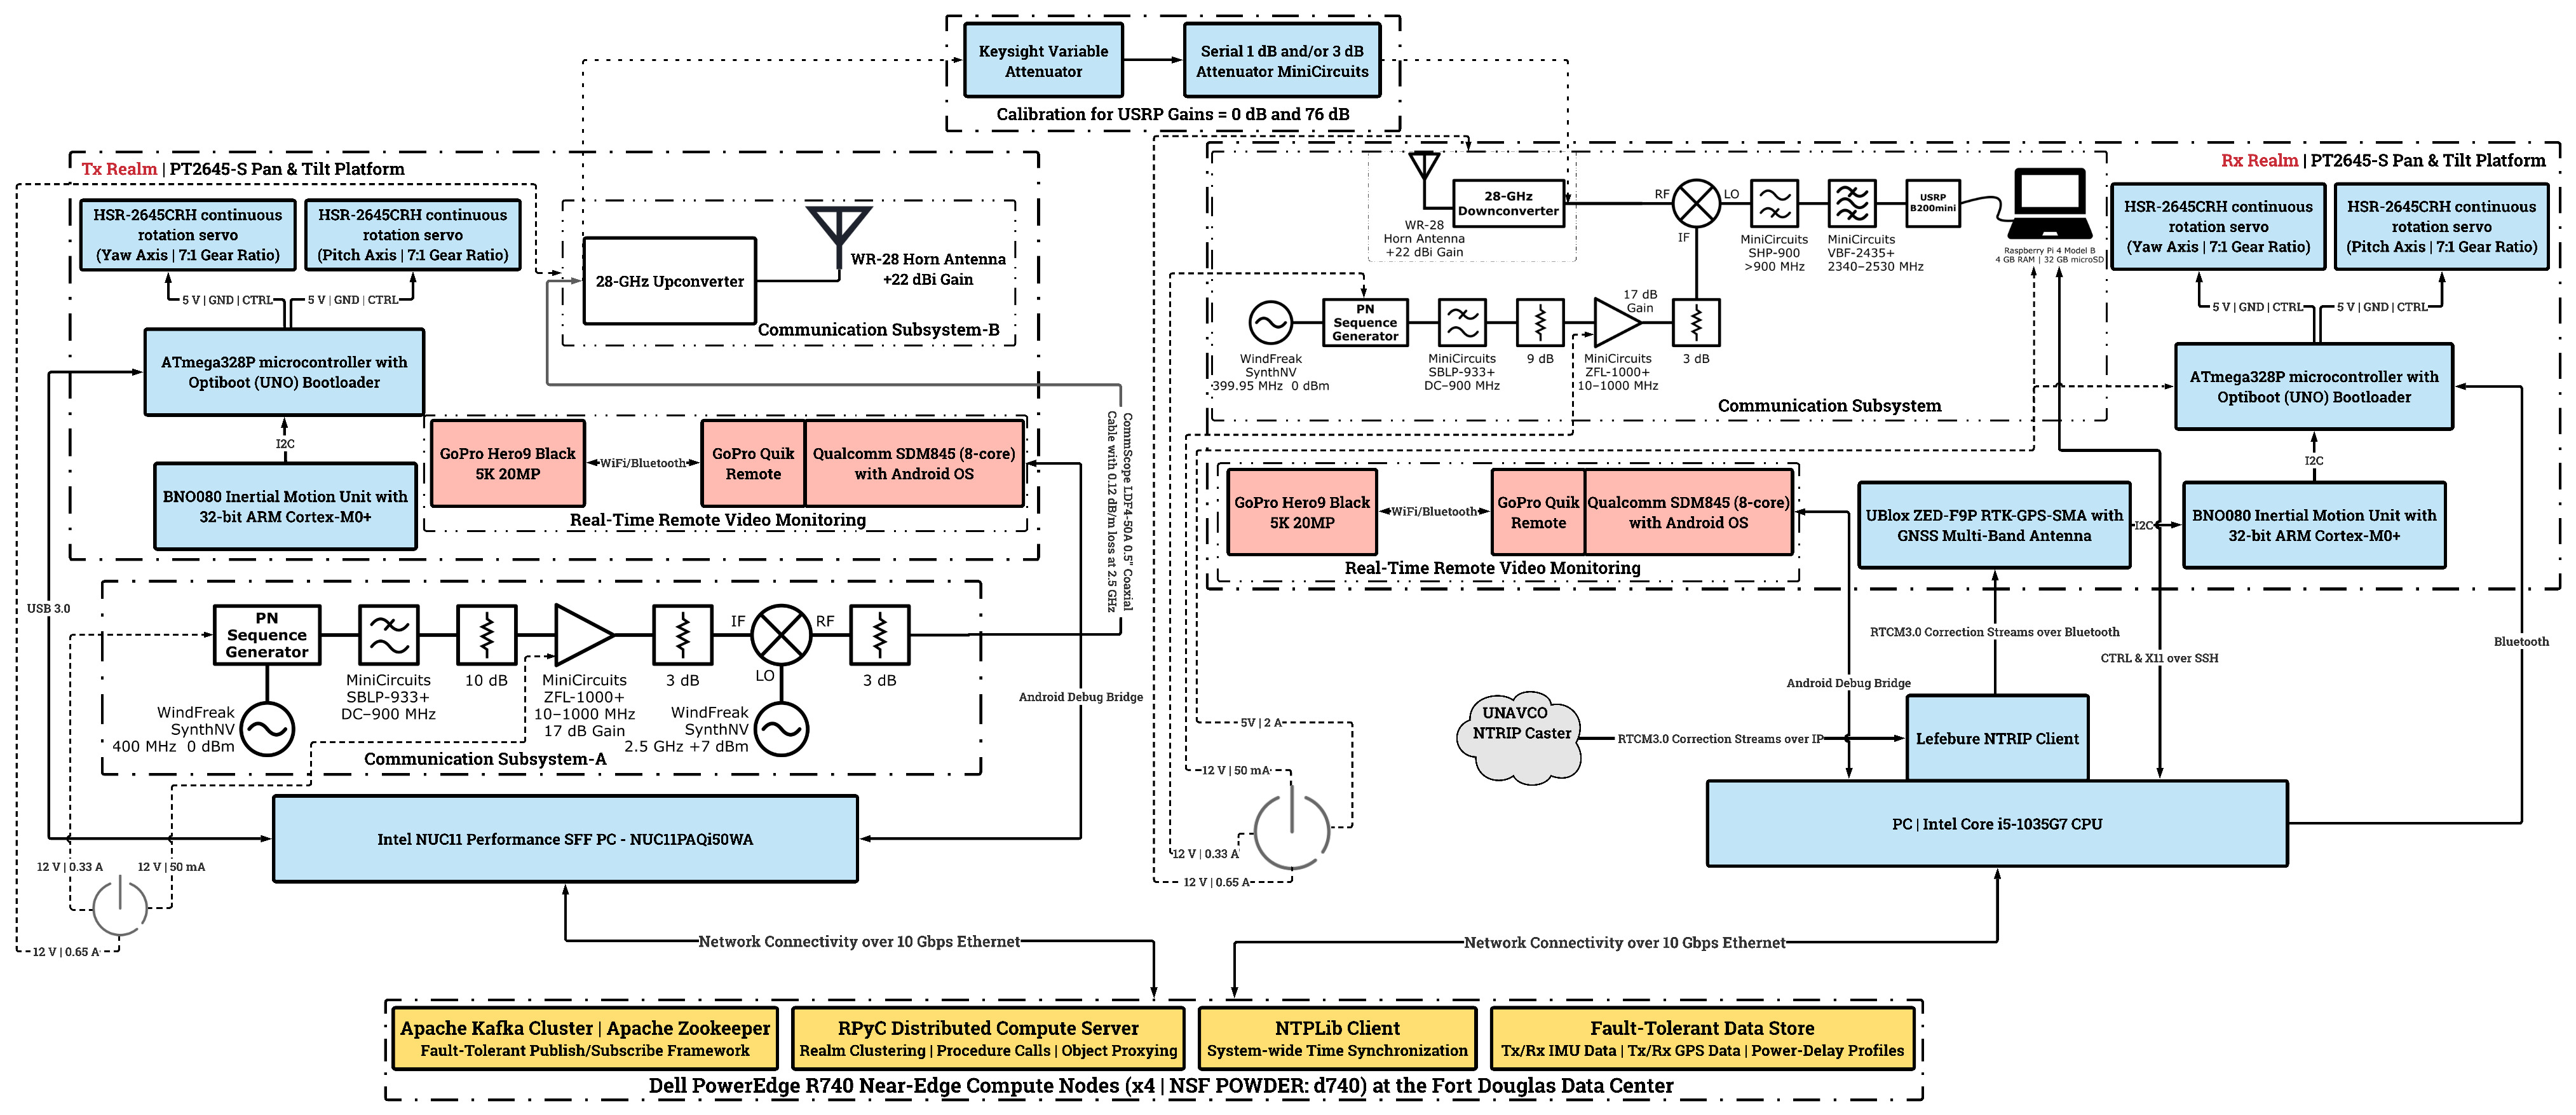
\includegraphics[width=1.0\textwidth]{figs/system_architecture.jpg}
    \vspace{-6mm}
    \caption{The architecture of our autonomous antenna alignment \& tracking platform with a sliding-correlator channel sounder.}
    \label{F1}
\end{figure*}

\noindent{\textbf{Channel Sounder}}: The measurement system employed a custom broadband sliding-correlator channel sounder at both the Tx and the Rx~\cite{Purdue}, each equipped with a Pseudorandom Noise (PN) sequence generator module producing the required known apriori signal for time-dilated cross-correlation studies, with the Rx module clocked at a slightly lower rate than the Tx; up-/down-converter to transition between the \SI{2.5}{\giga\hertz} and \SI{28}{\giga\hertz} regimes; a vertically polarized WR-28 directional horn antenna; and other commercially available components. This setup is depicted by the schematics in Fig.~\ref{F1} and is implemented by the circuits shown in Fig.~\ref{F2}, with the signal visualizations on a spectrum analyzer provided in Fig.~\ref{F3}. The operational specifications of the sounder are listed in Table~\ref{T2}, as detailed also in~\cite{Purdue}. At the Rx, complex-\SI{64}{} I/Q power-delay profiles are recorded onboard an SSD storage drive by a GNURadio sink on a Raspberry Pi SBC via a USRP B$200$mini SDR.

\noindent{\textbf{Alignment \& Tracking}}: First, to enable uninhibited rotational mobility for alignment and tracking in the horizontal and the vertical planes, as shown in Fig.~\ref{F1}, at both the Tx and the Rx, the WR-$28$ antenna is mounted on a PT-$2645$S open-loop pan-and-tilt unit, driven by $2{\times}$ HSR-$2645$CRH continuous rotation servos, each actuating either yaw (horizontal) or pitch (vertical) alignment. These servos are controlled via PWM signals from an ATMega$328$P microcontroller with the angular position (absolute and relative) feedback provided by a BNO$080$ inertial motion unit. This principal axes positioning subsystem demonstrates an average accuracy of \SI{1.1}{\degree} across all fine- \& coarse-grained yaw and pitch movements. Next, for seamless operations in V$2$X scenarios, the alignment platform is augmented with a geo-positioning subsystem consisting of a UBlox ZED-F$9$P GPS unit (with a GNSS multi-band antenna) wherein the positioning accuracy is enhanced by RTCM v$3.0$ RTK correction streams over NTRIP from a UNAVCO caster via a Lefebure client. Demonstrating an average $3$D accuracy of \SI{17}{\centi\meter}, the relevant data members captured by this geo-positioning unit---namely, the coordinate (latitude, longitude, and ellipsoidal altitude), the horizontal speed \& acceleration, and the heading, are communicated to the microcontroller as NMEA-0183 messages over an I2C serial peripheral bus.
\begin{table*} [tb]
	\centering
	\scriptsize
	\begin{tabular}{|l||l|}
		\hline
		Carrier Frequency & \SI{28}{\giga\hertz}\\
		\hline
		PN Chip Sequence Length & \SI{2047}{}\\
		\hline
		RF Bandwidth & \SI{800}{\mega\hertz}\\
		\hline
		Tx Chip Rate & \SI{400}{\mega{cps}}\\
		\hline
		Temporal Resolution & \SI{2.5}{\nano\second}\\
		\hline
		Rx Chip Rate & \SI{399.95}{\mega{cps}}\\
		\hline
		Tx Power & \SI{23}{\deci\bel{m}}\\
		\hline
		Tx/Rx Antenna Gain & \SI{22}{\deci\bel{i}}\\
		\hline
		Nominal Tx/Rx Antenna HPBW & \SI{15}{\degree}\\
		\hline
		Measured Tx/Rx Azimuth HPBW & \SI{10.1}{\degree}\\
		\hline
		Measured Tx/Rx Elevation HPBW & \SI{11.5}{\degree}\\
		\hline
		Maximum Measurable Pathloss & \SI{182}{\decibel}\\
		\hline
		GNURadio Sink Center Frequency & \SI{2.5}{\giga\hertz}\\
		\hline
		USRP Gain & \SI{76}{\decibel}\\
		\hline
		USRP Sampling Rate & \SI{2}{\mega{sps}}\\
		\hline
	\end{tabular}
	\vspace{-1mm}
	\caption{The specifications of the sliding-correlator channel sounder used in our measurement campaign on NSF POWDER.}
	\label{T3}
\end{table*}

Since our measurement system revolves around a decoupled design with the alignment and tracking platform replicated at both the Tx and the Rx, a centralized nerve-center handles asynchronous module registration \& de-registration via RPyC object proxying, global timing synchronization via NTP, and coordination between the Tx and Rx over fault-tolerant Apache Kafka messaging middleware. With Apache Zookeeper broker management, the samples generated by the principal axes positioning and geo-positioning subsystems are shared over Kafka message queues: the Tx subscribes to the alignment and geo-location messages published by the Rx, and vice-versa, resulting in a scalable event-driven modular architecture. Corroborated both onsite and in the laboratory, this publish-subscribe framework facilitates an average beam-steering response time of \SI{27.8}{\milli\second}, evaluated over \SI{12870}{} interactions. With system monitoring provided over an Android debug bridge and system troubleshooting enabled via serial communication interfaces, our platform demonstrates remote orchestration capabilities: a critical necessity for V$2$X propagation modeling. To augment these remote monitoring and troubleshooting features further, a GNURadio Qt GUI time-sink (with dynamic trigger levels) allows for real-time visualization of the recorded power-delay profiles over an ad-hoc WLAN with the Raspberry Pi SBC; additionally, via the Plotly Dash and MapBox APIs, the Tx and Rx geo-locations are annotated with their relative alignment accuracies and visualized in real-time at a control terminal for onsite validation of the routes traversed on NSF POWDER.
\vspace{-4mm}

% Measurement campaign description and Data post-processing procedural explanation
\section{Measurements \& Post-Processing}\label{S3}
In this section, we discuss the operations involved in our \SI{28}{\giga\hertz} V$2$X measurement campaign on the NSF POWDER testbed. First, we describe the system calibration process; next, we outline the onsite system deployment procedure; and finally, we detail the post-processing steps involved in setting up the power-delay profiles recorded at the Rx for pathloss evaluations, multipath component extraction and parameter estimation via SAGE, and spatial consistency analyses.

\noindent{\textbf{Pre-deployment Calibration}}: After the Tx and Rx circuits for the sliding correlator channel sounder have been implemented as illustrated in Figs.~\ref{F2}(a) and~\ref{F2}(d), a calibration procedure is carried out onsite to map the power calculated from the power-delay profiles recorded by the USRP to reference measured power levels. Calibrating the measurement system before deployment ensures accurate Rx power calculations in the presence of imperfect circuit components, e.g., the Commscope LDF$4$-$50$A \SI{0.5}{{"}} coaxial cables employed at the Tx exhibit losses of up to \SI{0.12}{\deci\bel\per\meter} at \SI{2.5}{\giga\hertz}. Under \SI{0}{\deci\bel} and \SI{76}{\deci\bel} USRP gains, using a Keysight variable attenuator, the recorded power-delay profiles are processed to determine the calculated power values mapped to the reference power levels: the results of this procedure are studied in Sec.~\ref{S4}.
\begin{figure*}[t]
    \centering
    \begin{tabular}{cc}
        \begin{minipage}{0.522\linewidth} 
        	\centering
            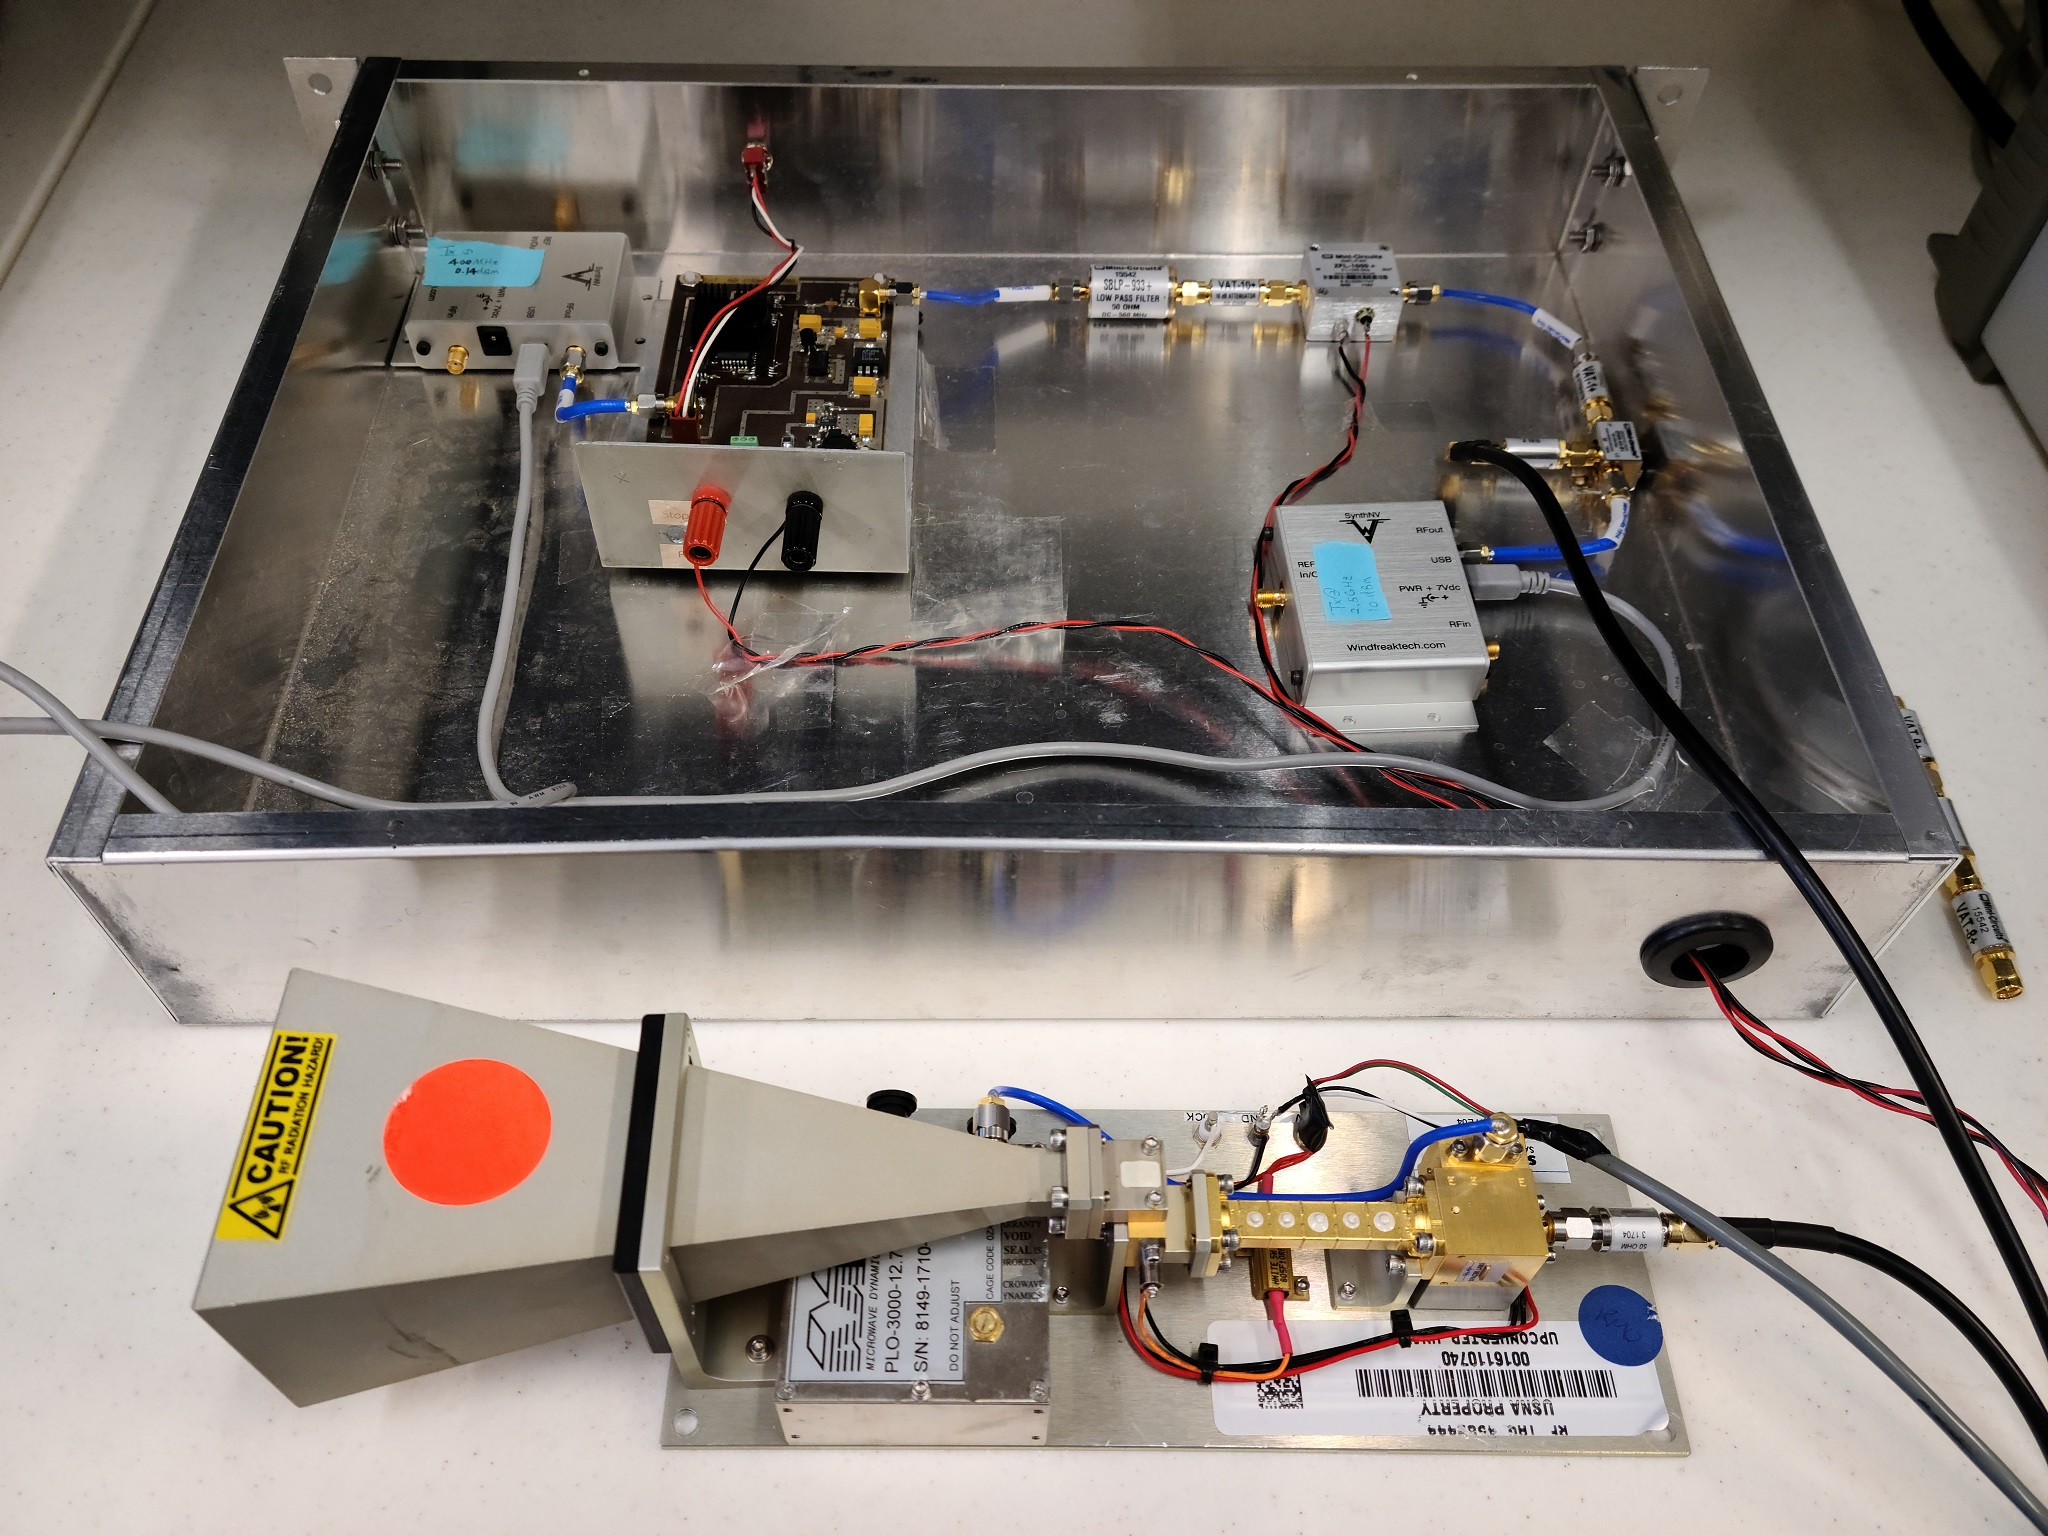
\includegraphics[width=0.9\linewidth]{figs/tx_comm_setup.jpg}
            \\ [0.55ex]
            \centering
            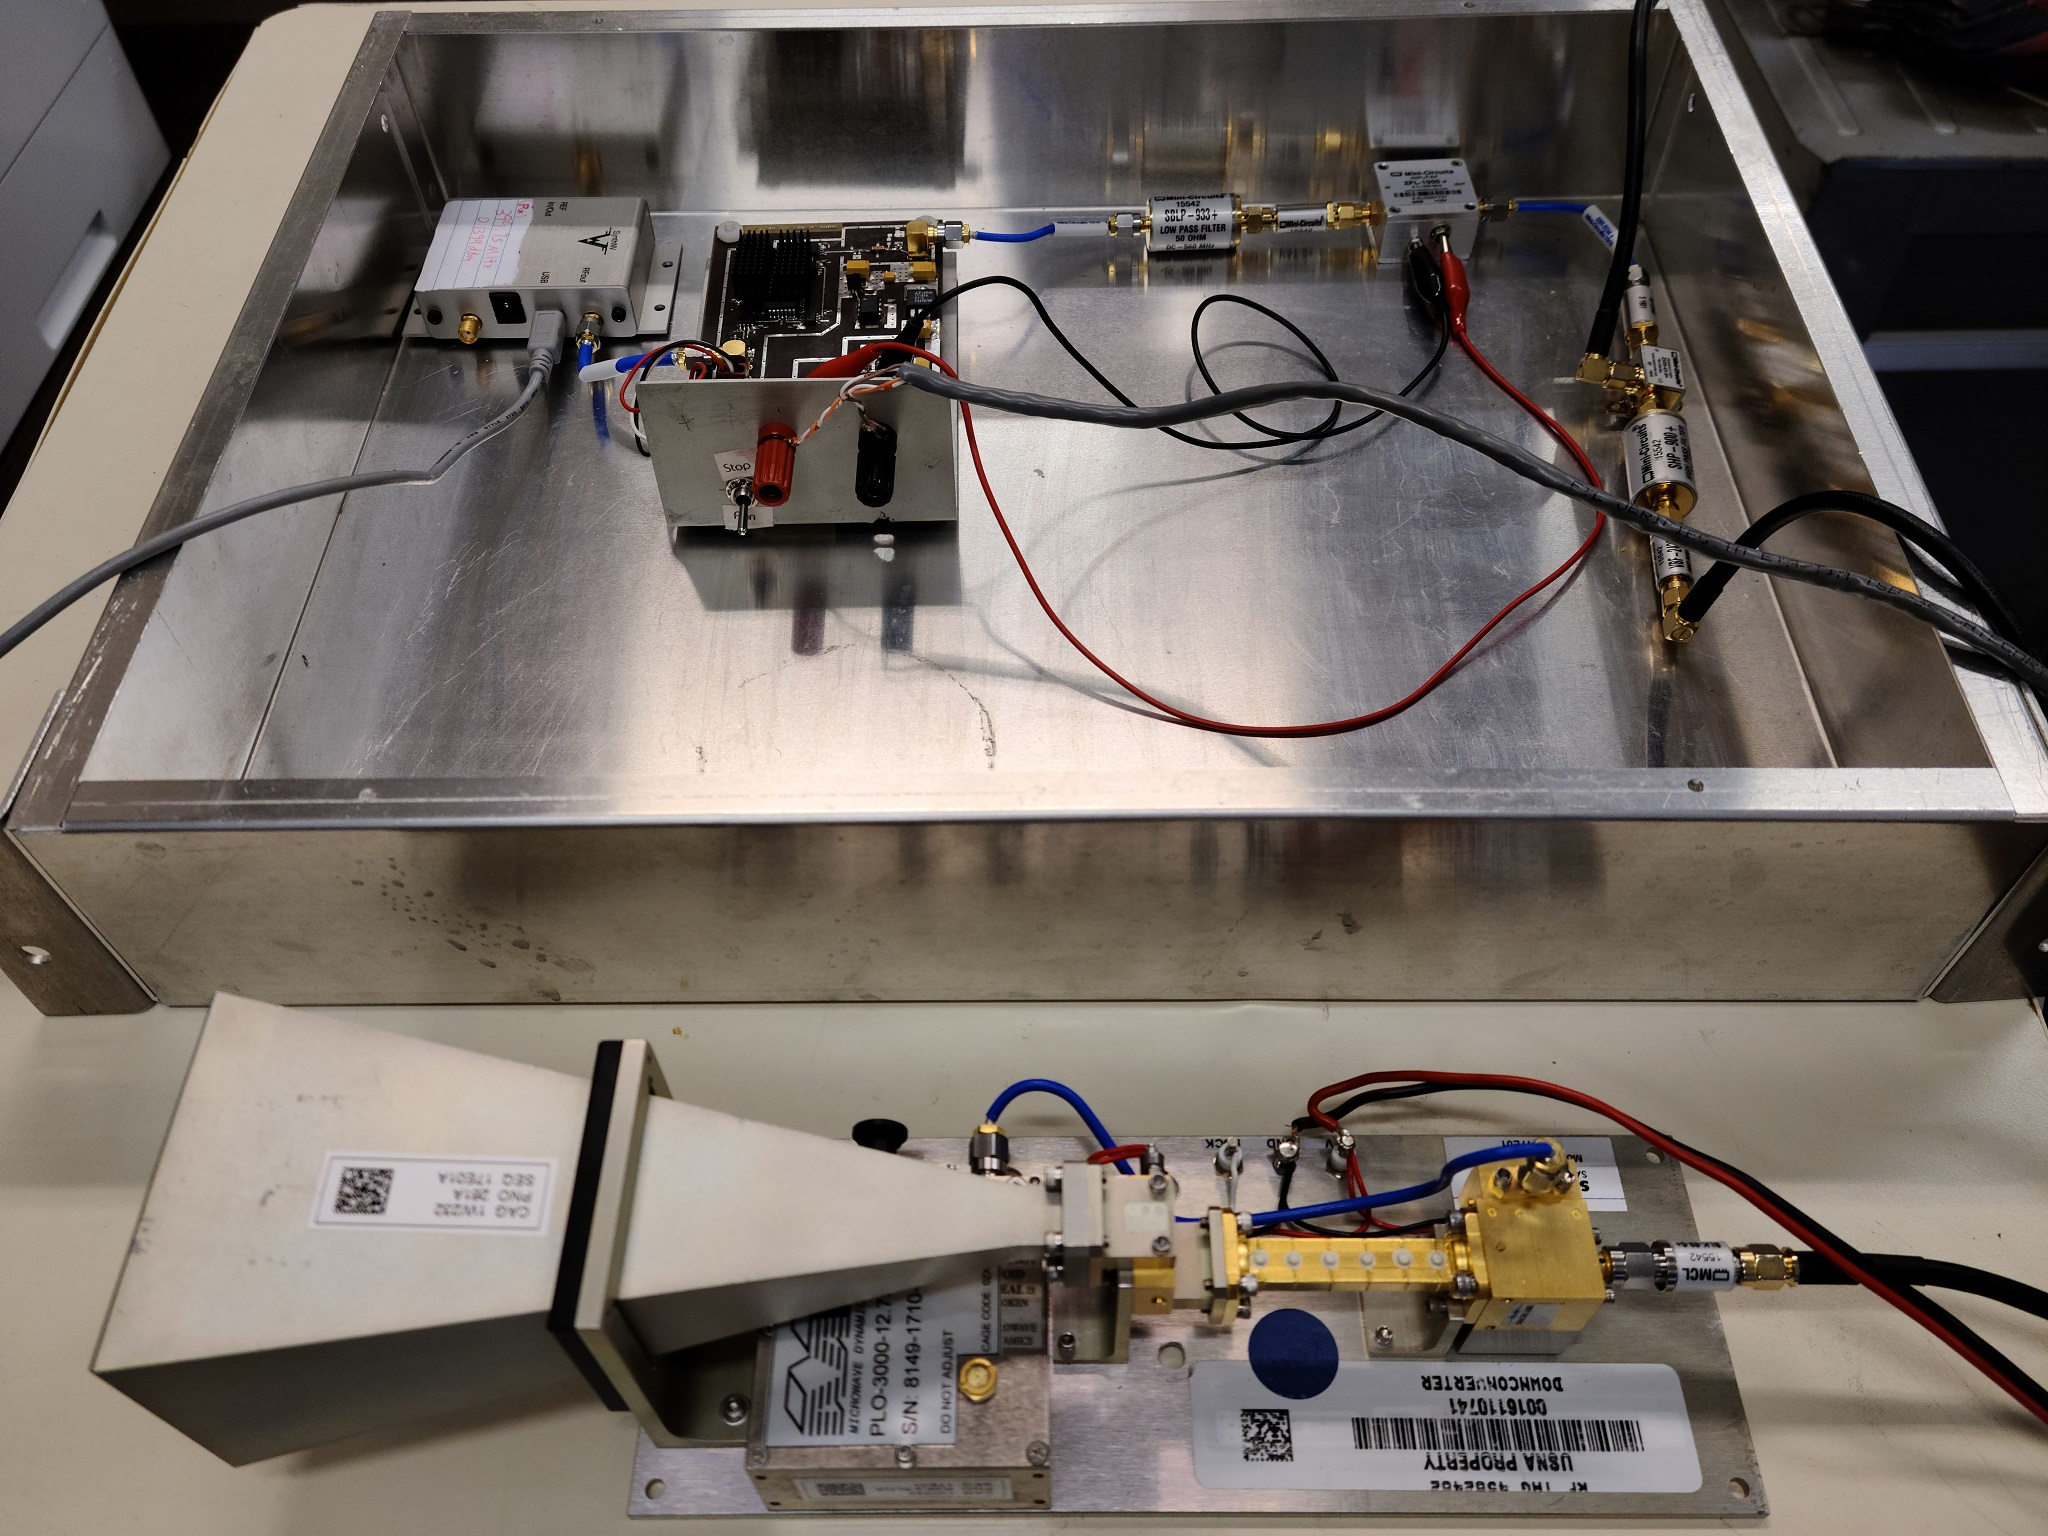
\includegraphics[width=0.9\linewidth]{figs/rx_comm_setup.jpg}
        \end{minipage}&
        \hspace{-10mm}
        \begin{minipage}{0.478\linewidth}
        	\centering
            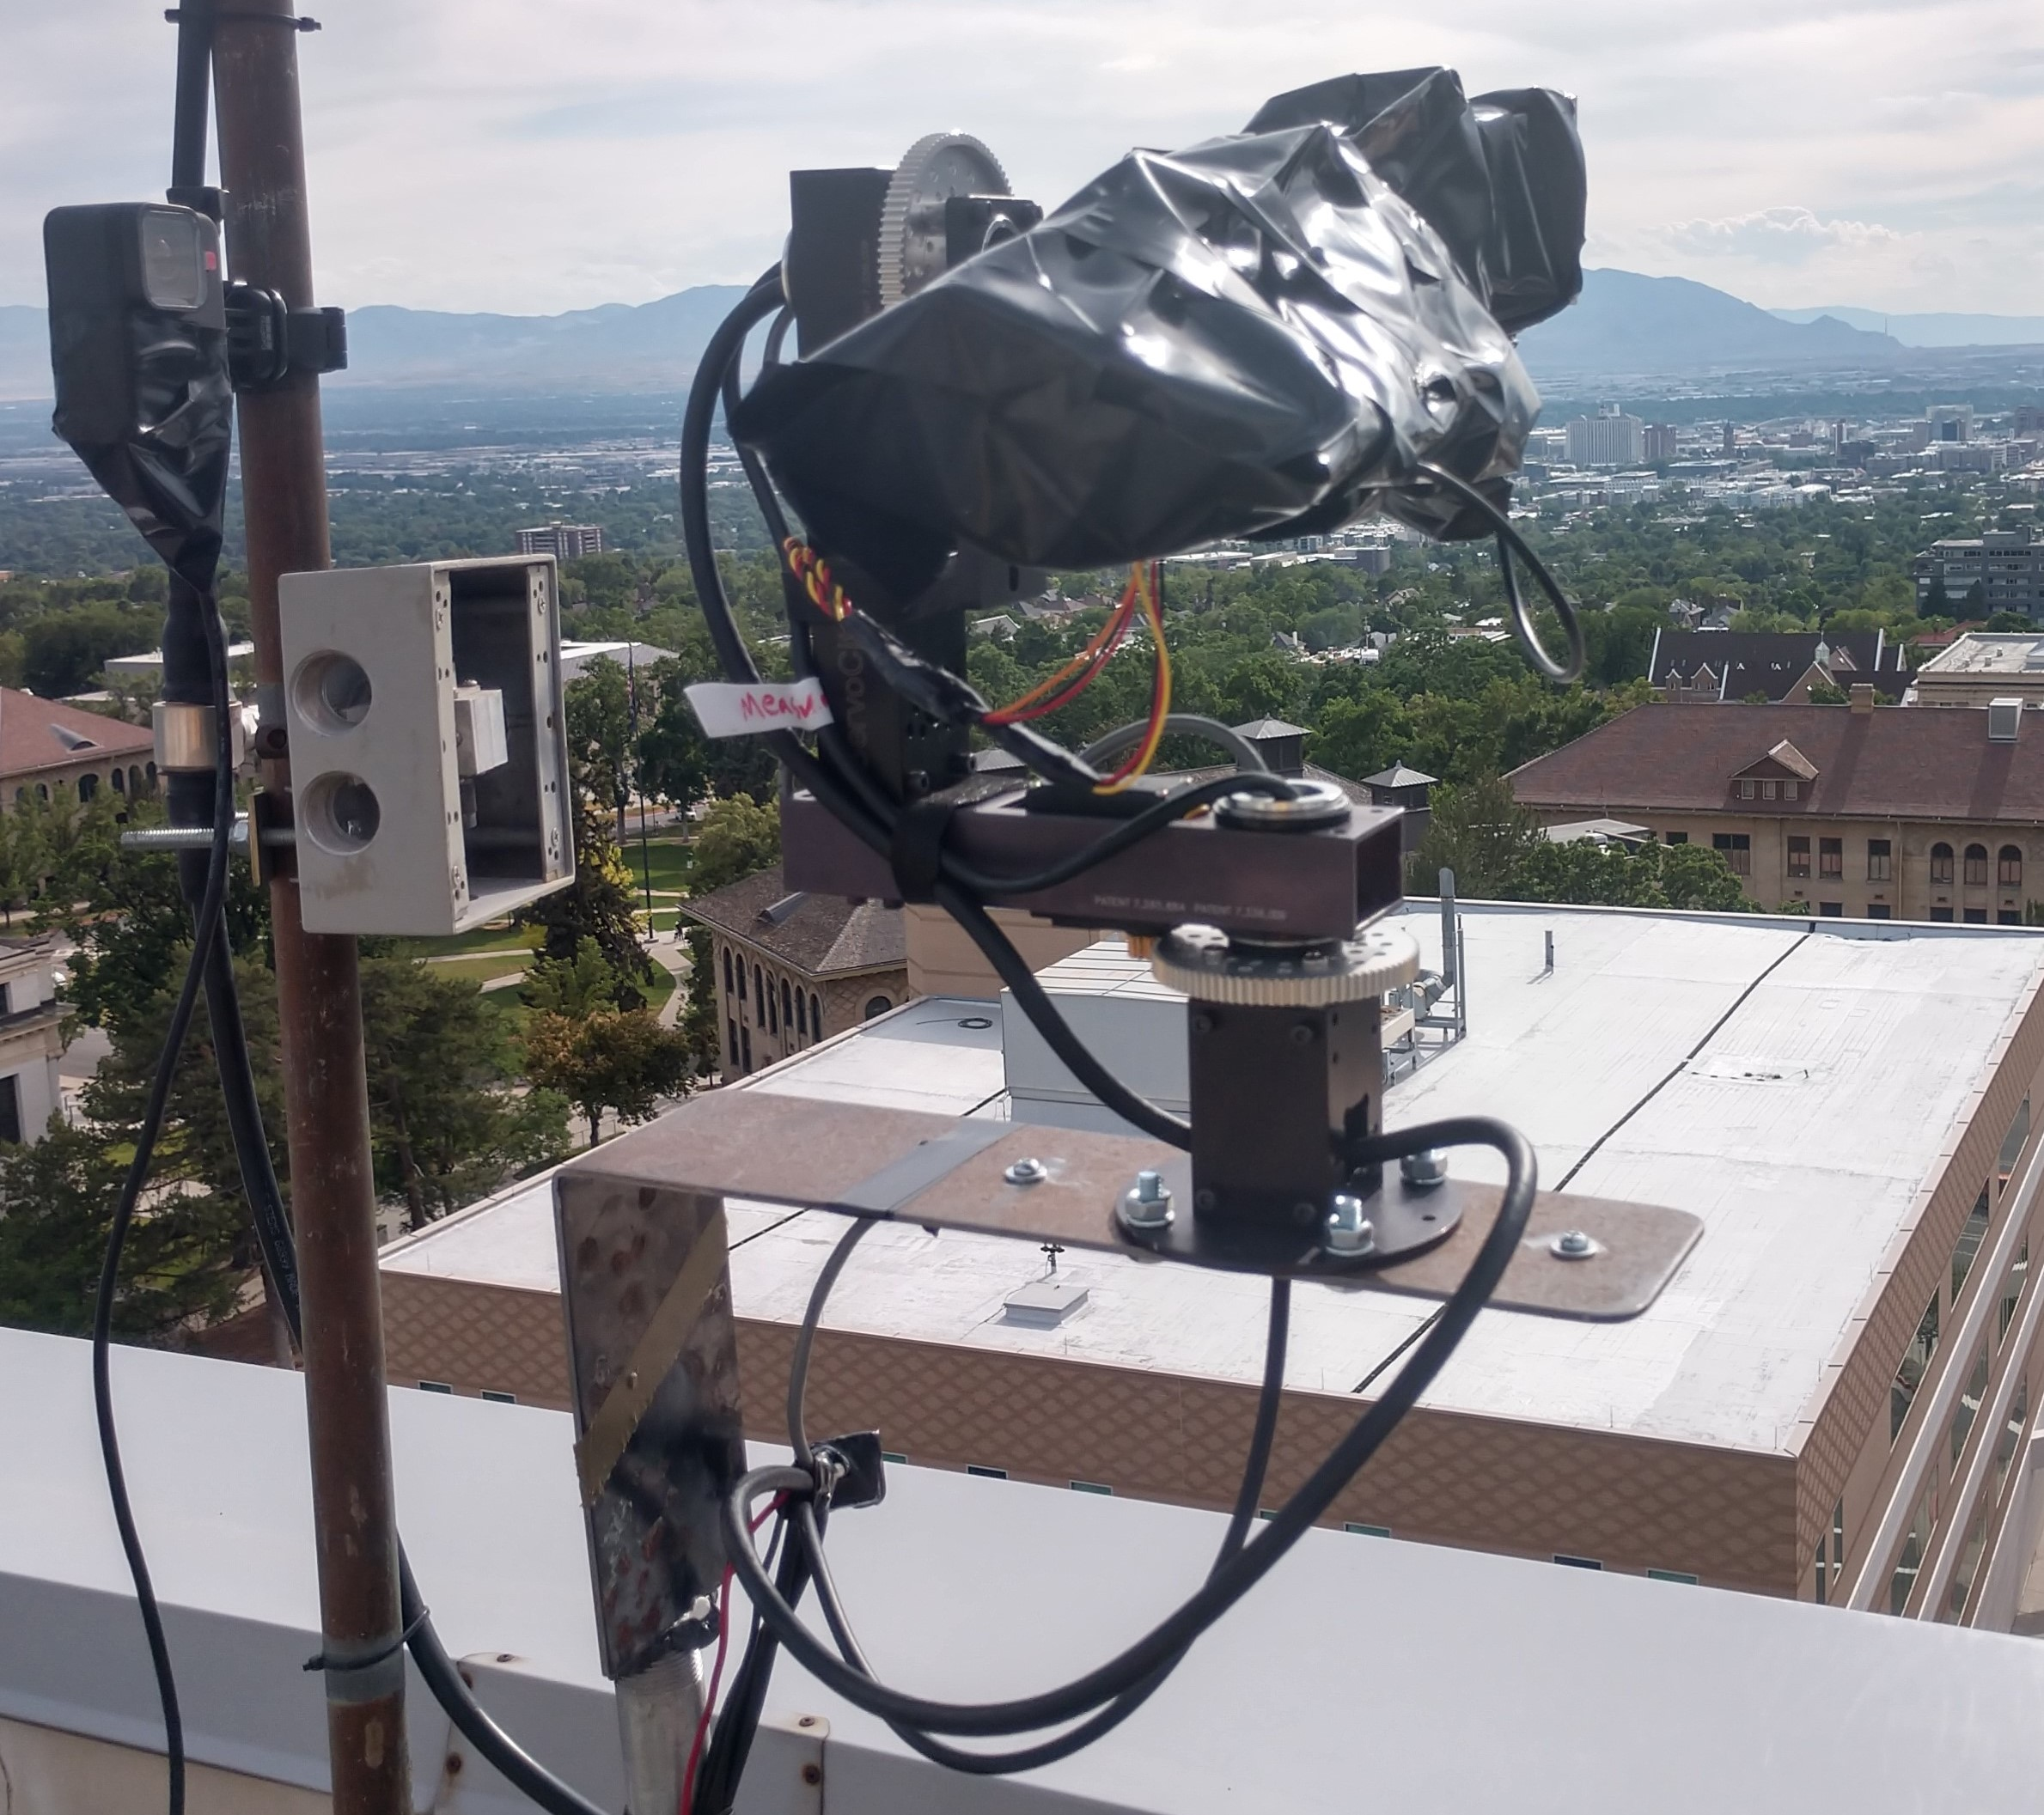
\includegraphics[width=0.9\linewidth]{figs/tx_deployment_browning.jpg}
            \\ [0.55ex]
            \centering
            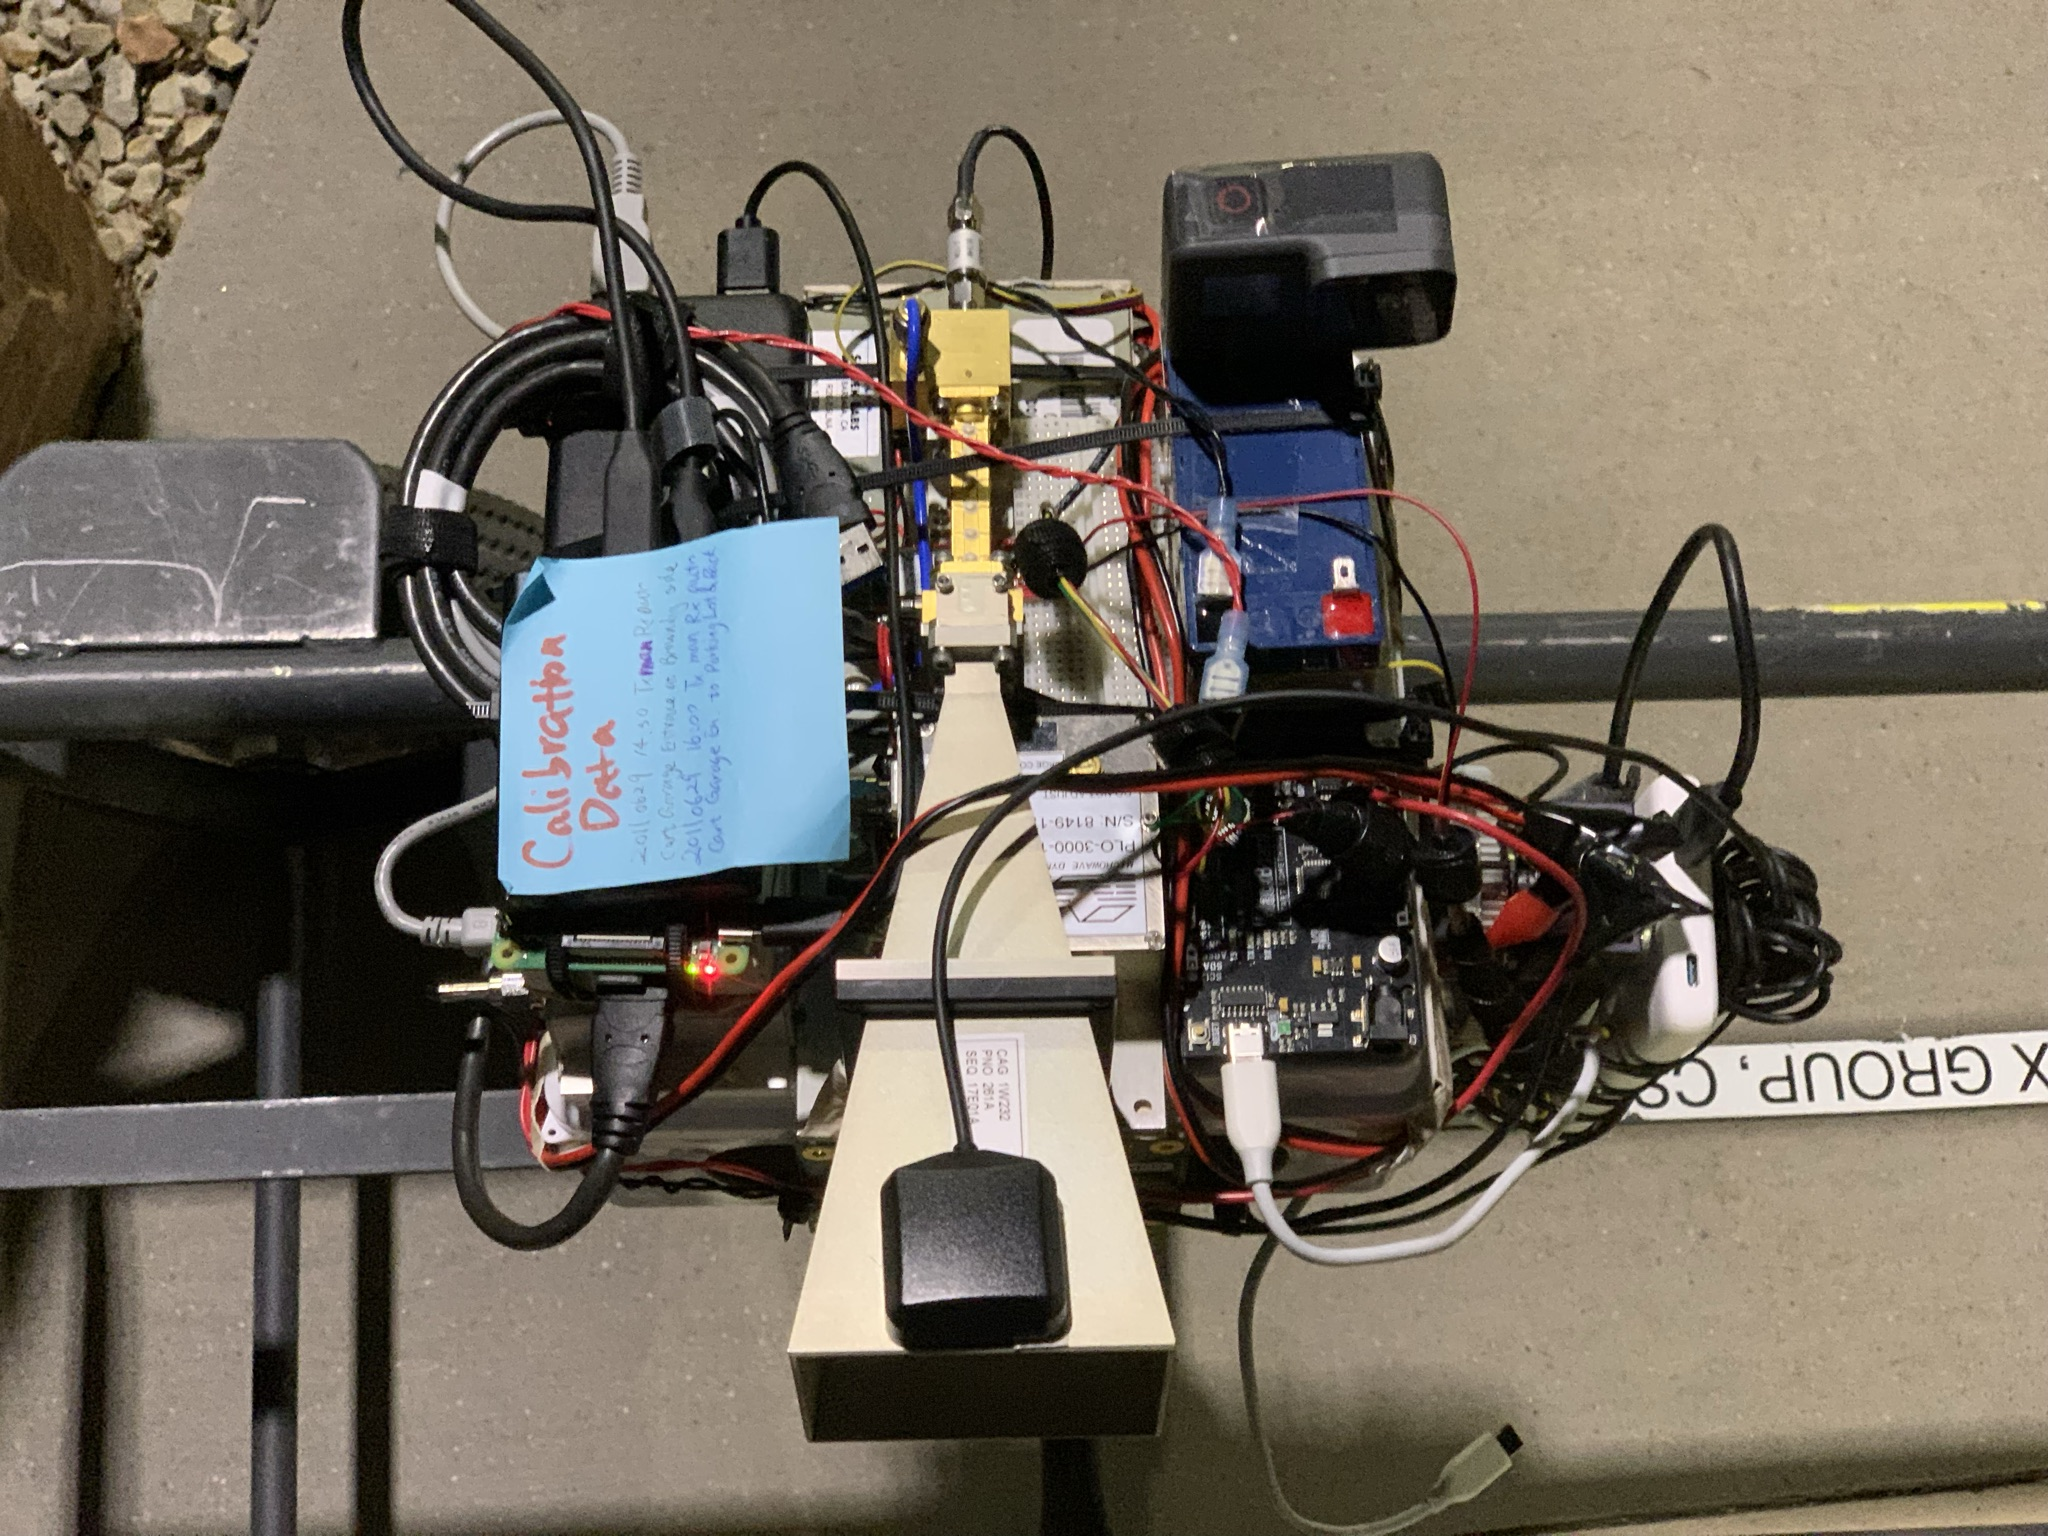
\includegraphics[width=0.9\linewidth]{figs/rx_cart_deployment.jpg}
        \end{minipage}
    \end{tabular}
    \caption{Clockwise from top-left: The Tx circuit with a \SI{28}{\giga\hertz} up-converter, a WR-$28$ directional horn antenna, and other commercially available parts (a); the deployment of the Tx atop the William Browning building: the sounder circuits are housed in a climate-controlled enclosure with the antenna mounted on the pan-and-tilt platform (b); the deployment of the Rx mounted on a push-cart (or a minivan) and pushed (or driven) around onsite (c); the Rx circuit with a \SI{28}{\giga\hertz} down-converter, a WR-$28$ directional horn antenna, USRP B$200$mini SDR, Raspberry Pi SBC, and other commercially available parts (d).}
    \label{F2}
\end{figure*}
\begin{figure*}[t]
    \begin{tabular}{cc}
        \begin{minipage}{0.5\linewidth} 
            \centering
            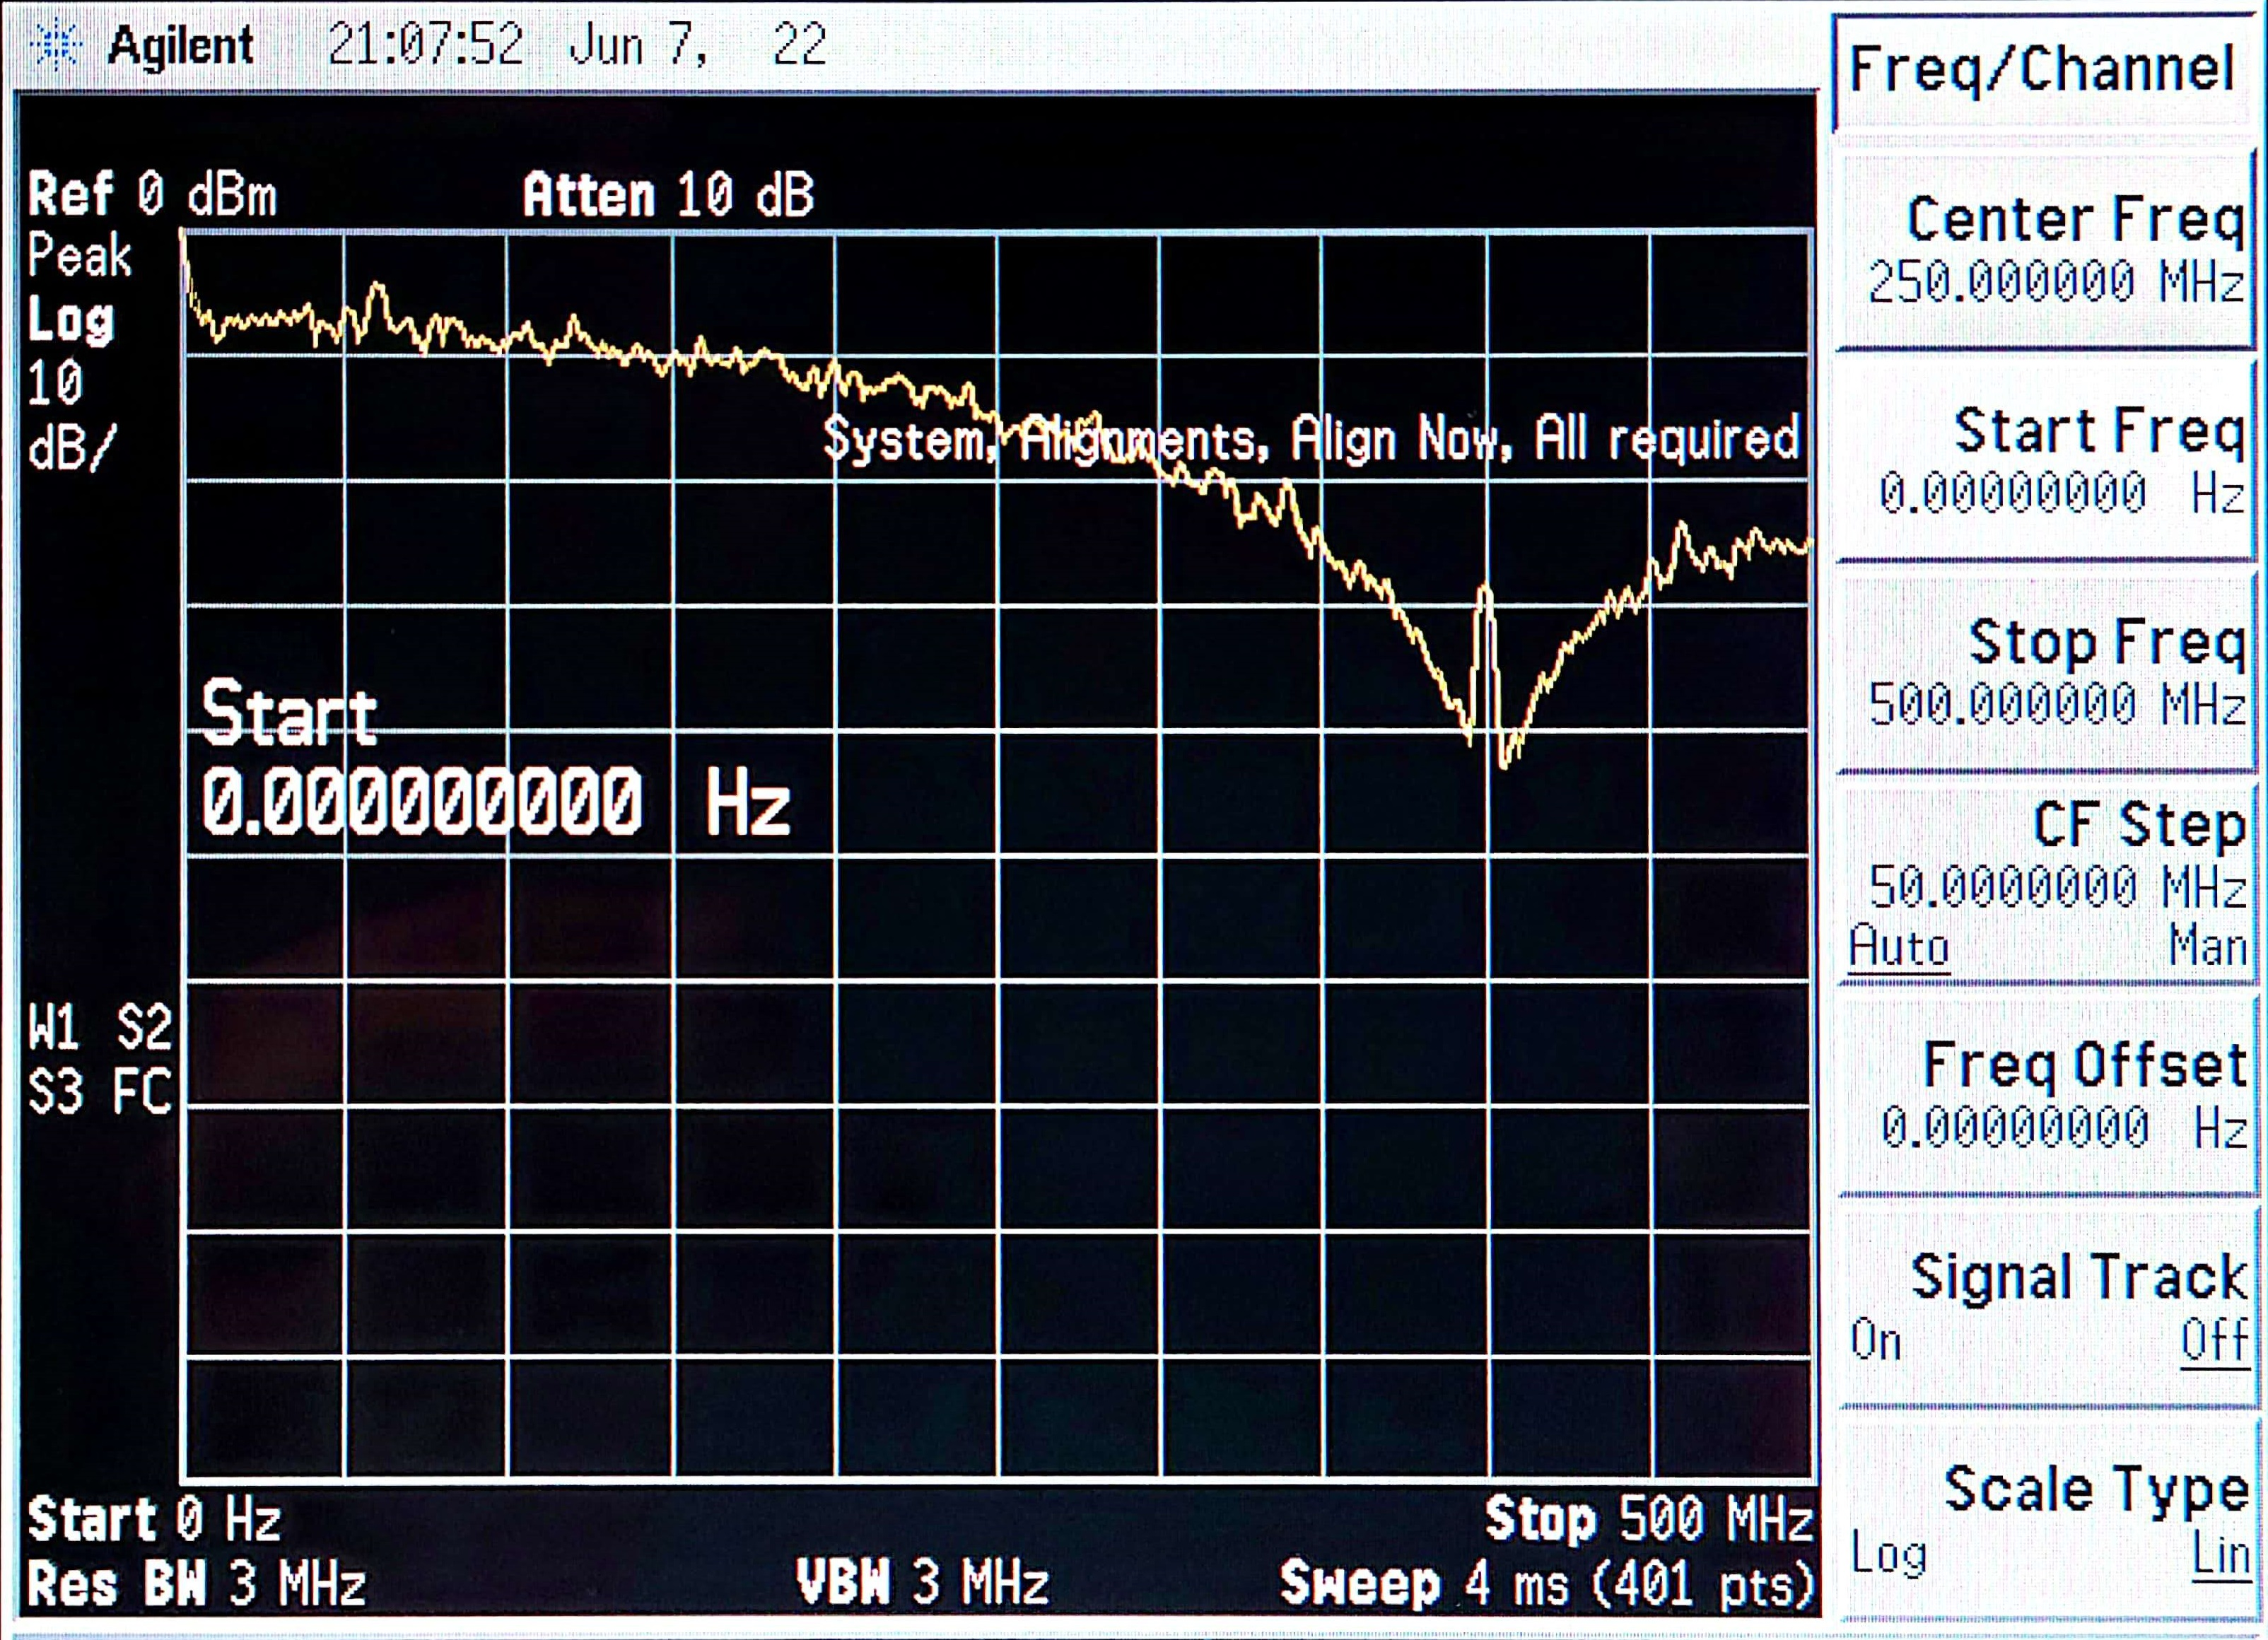
\includegraphics[width=0.9\linewidth]{backup_figs/PN_Output_400MHz_CLK.jpg}
            \\ [0.5ex]
            \centering
            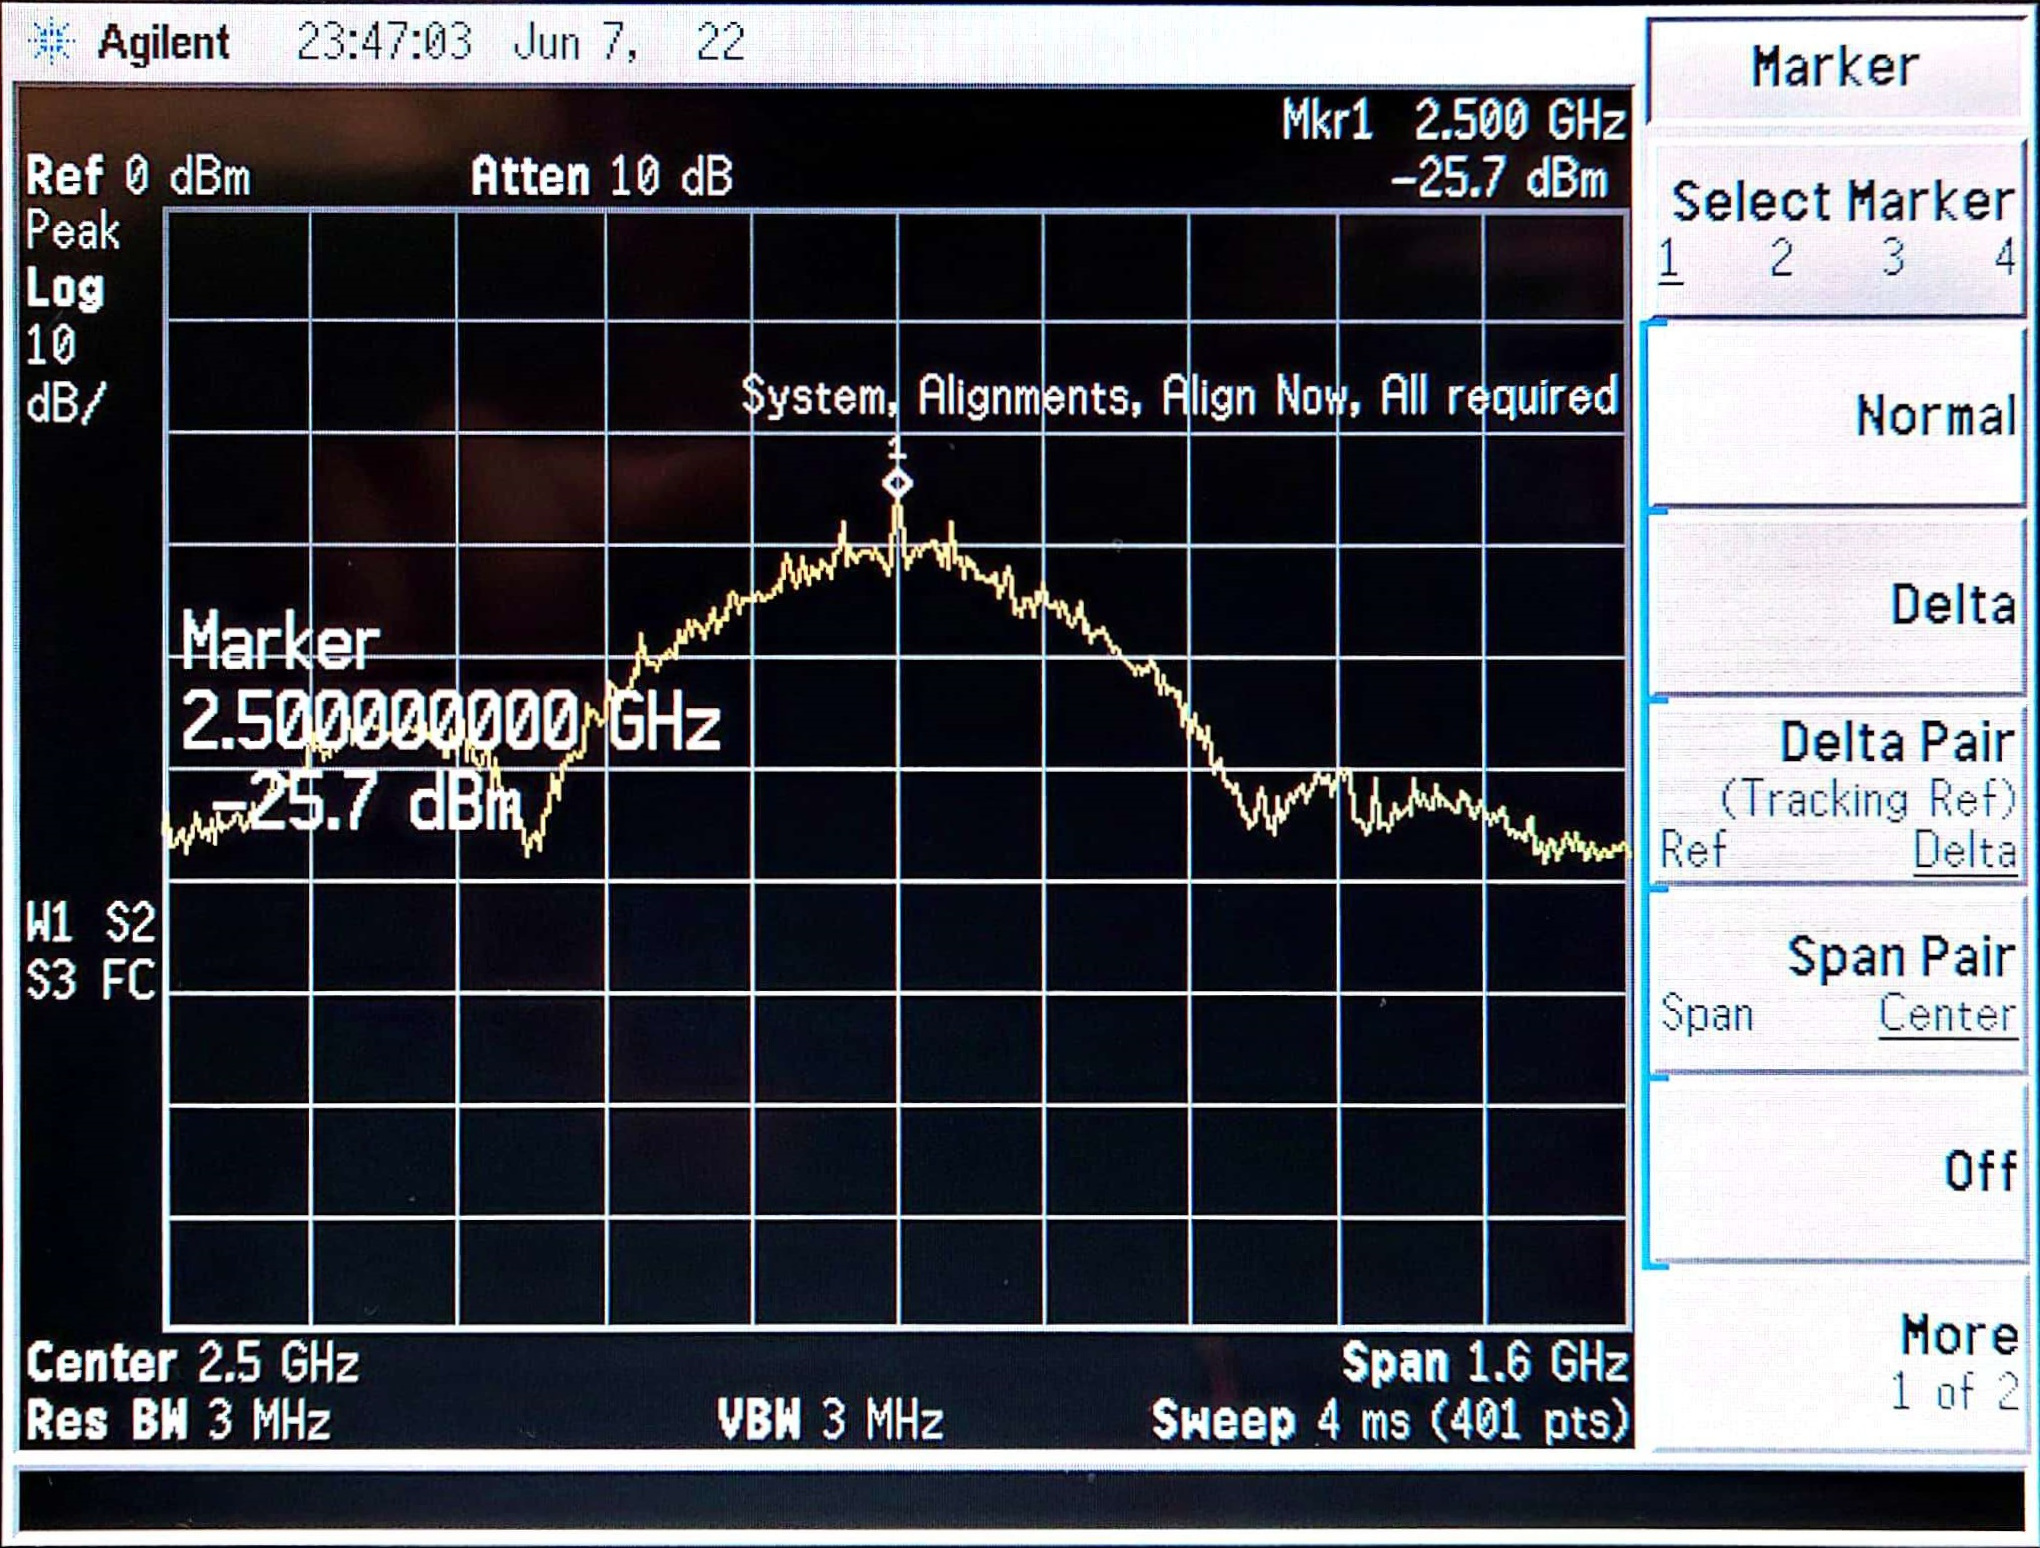
\includegraphics[width=0.9\linewidth]{backup_figs/Rx_Signal_IF.jpg}
            \\ [0.5ex]
            \centering
            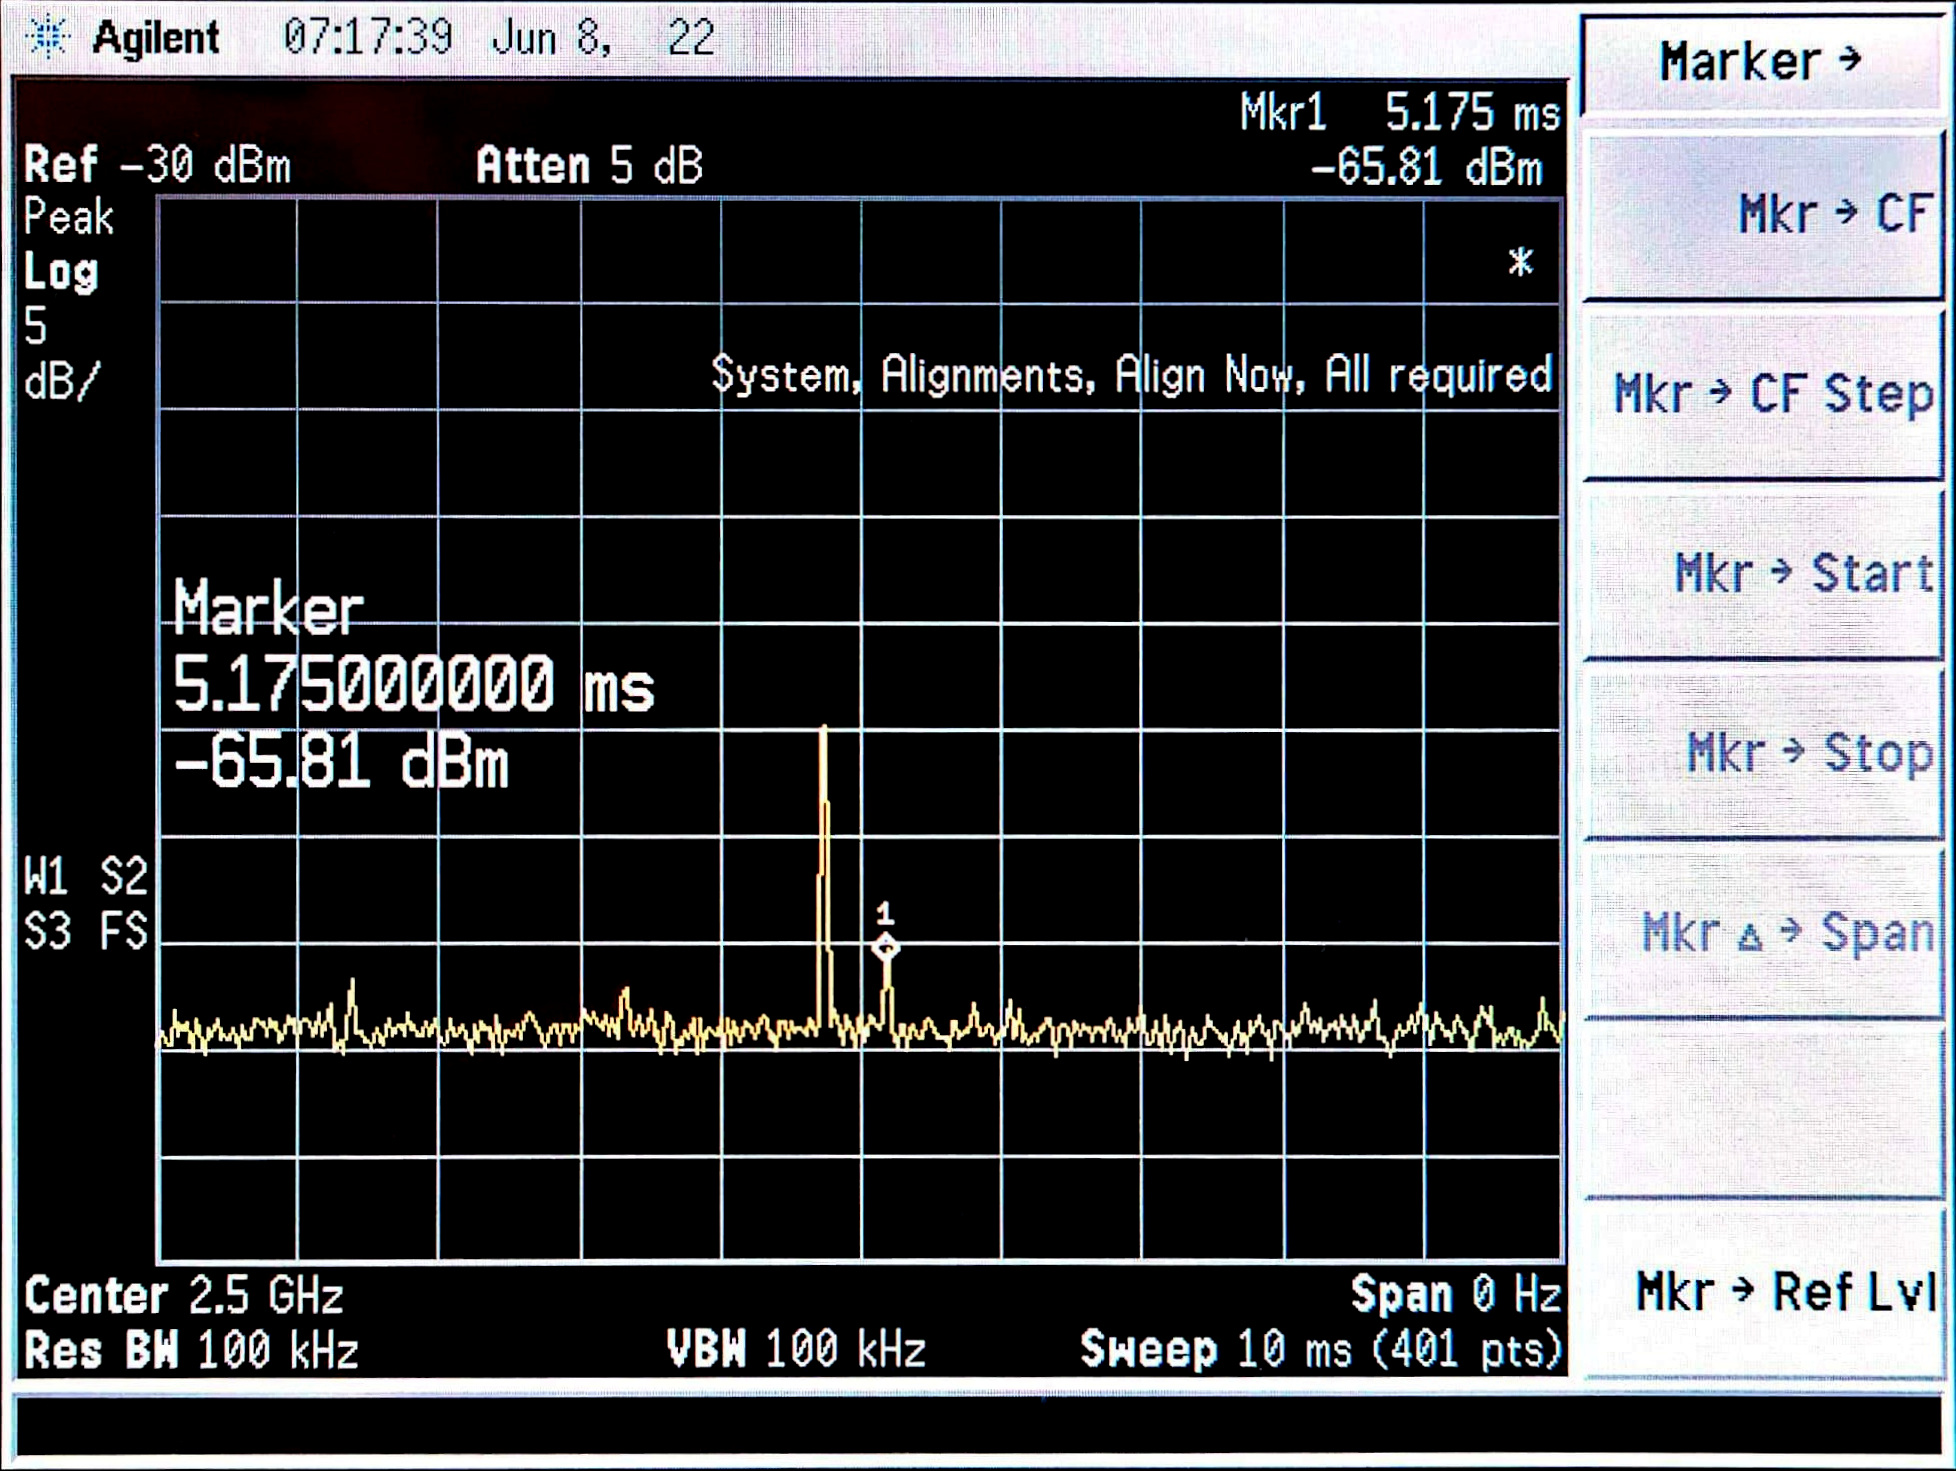
\includegraphics[width=0.9\linewidth]{backup_figs/PDP_Reflected.jpg}
        \end{minipage}&
        \hspace{-6mm}
        \begin{minipage}{0.5\linewidth}
            \centering
            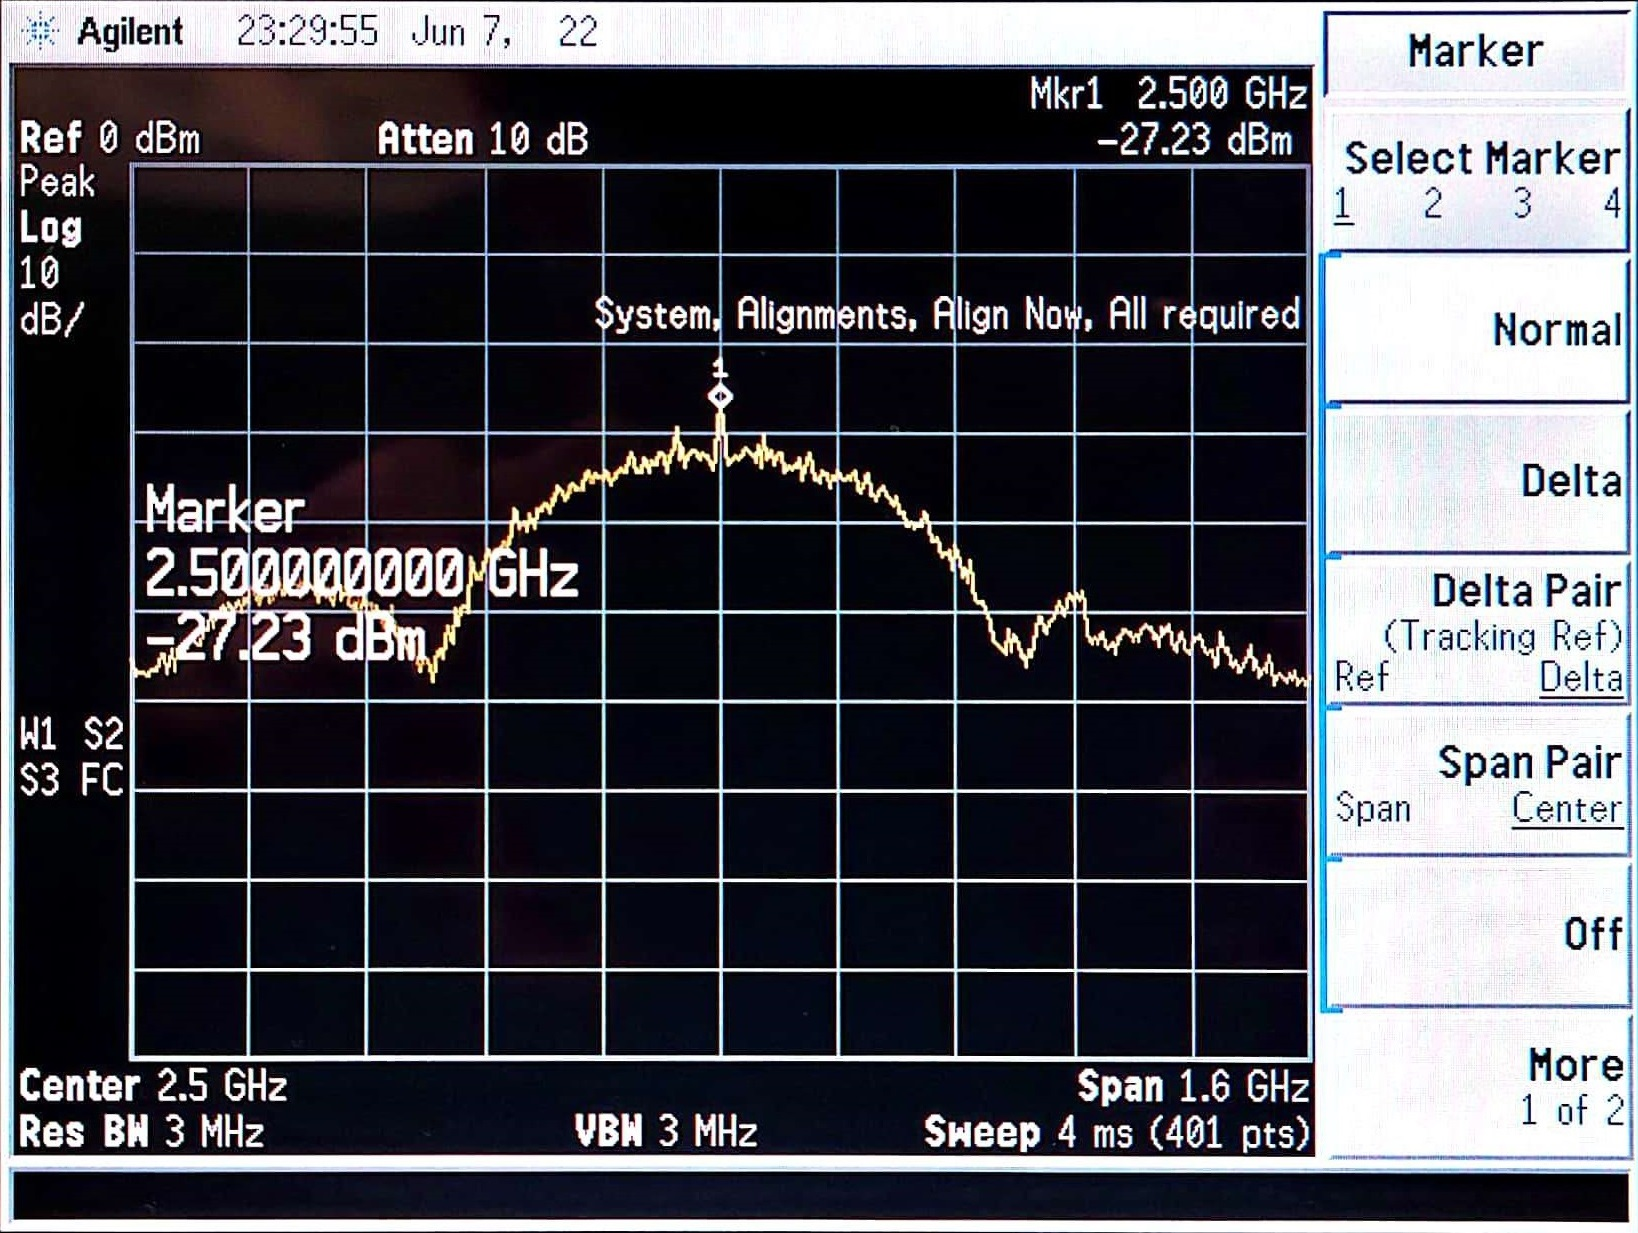
\includegraphics[width=0.9\linewidth]{backup_figs/Tx_Signal_IF.jpg}
            \\ [0.5ex]
            \centering
            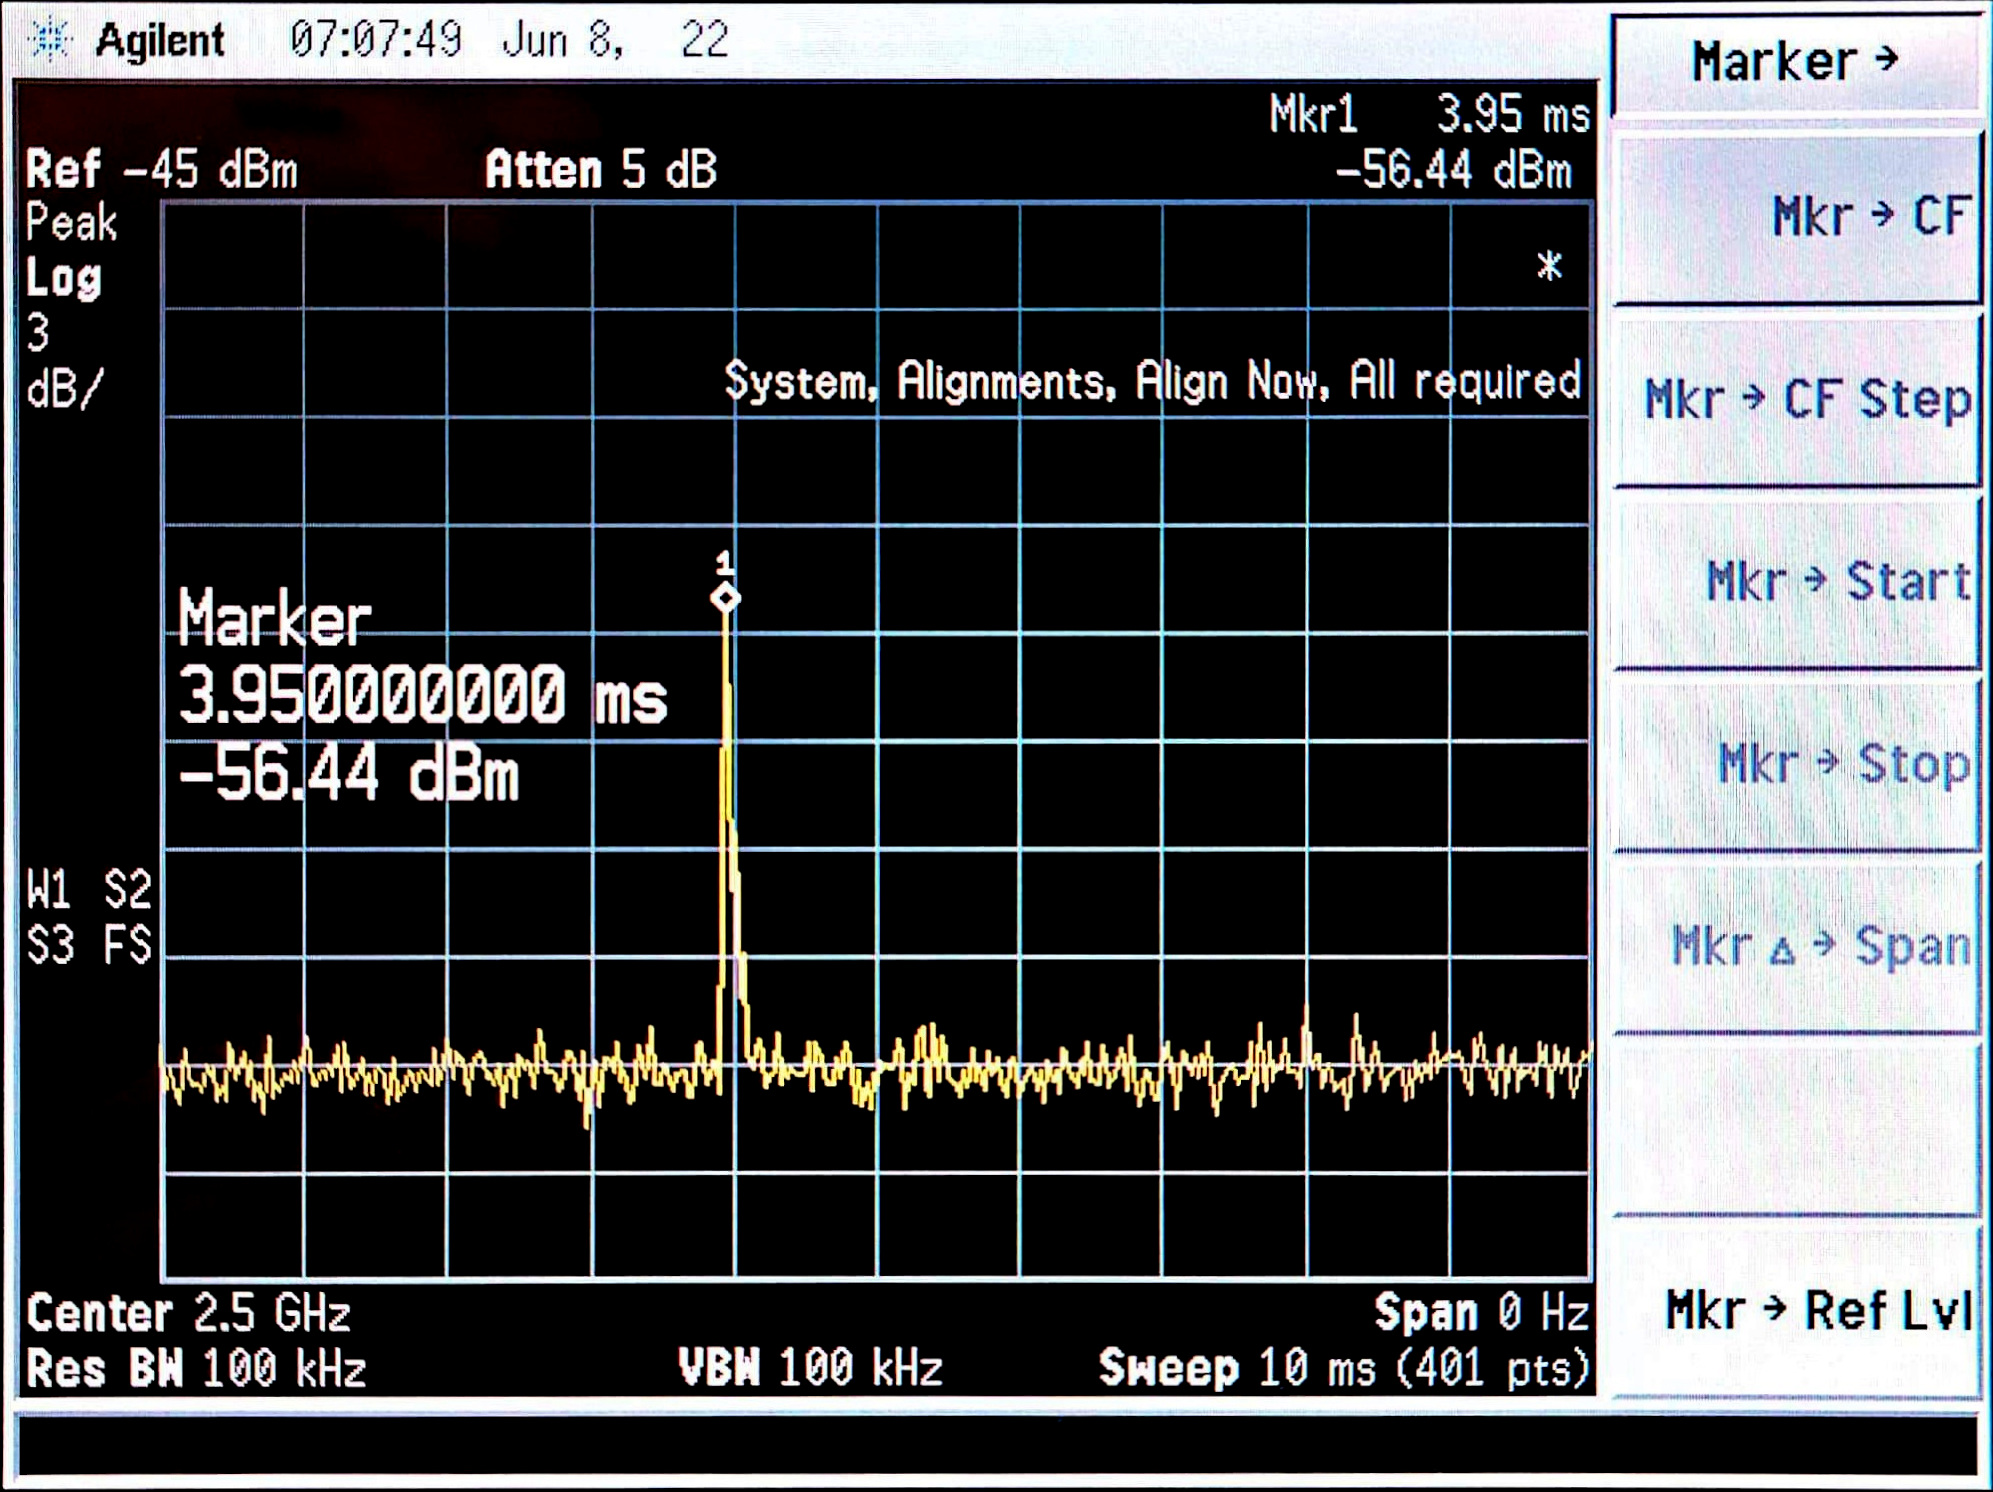
\includegraphics[width=0.9\linewidth]{backup_figs/PDP_Dominant_LoS.jpg}
            \\ [0.5ex]
            \centering
            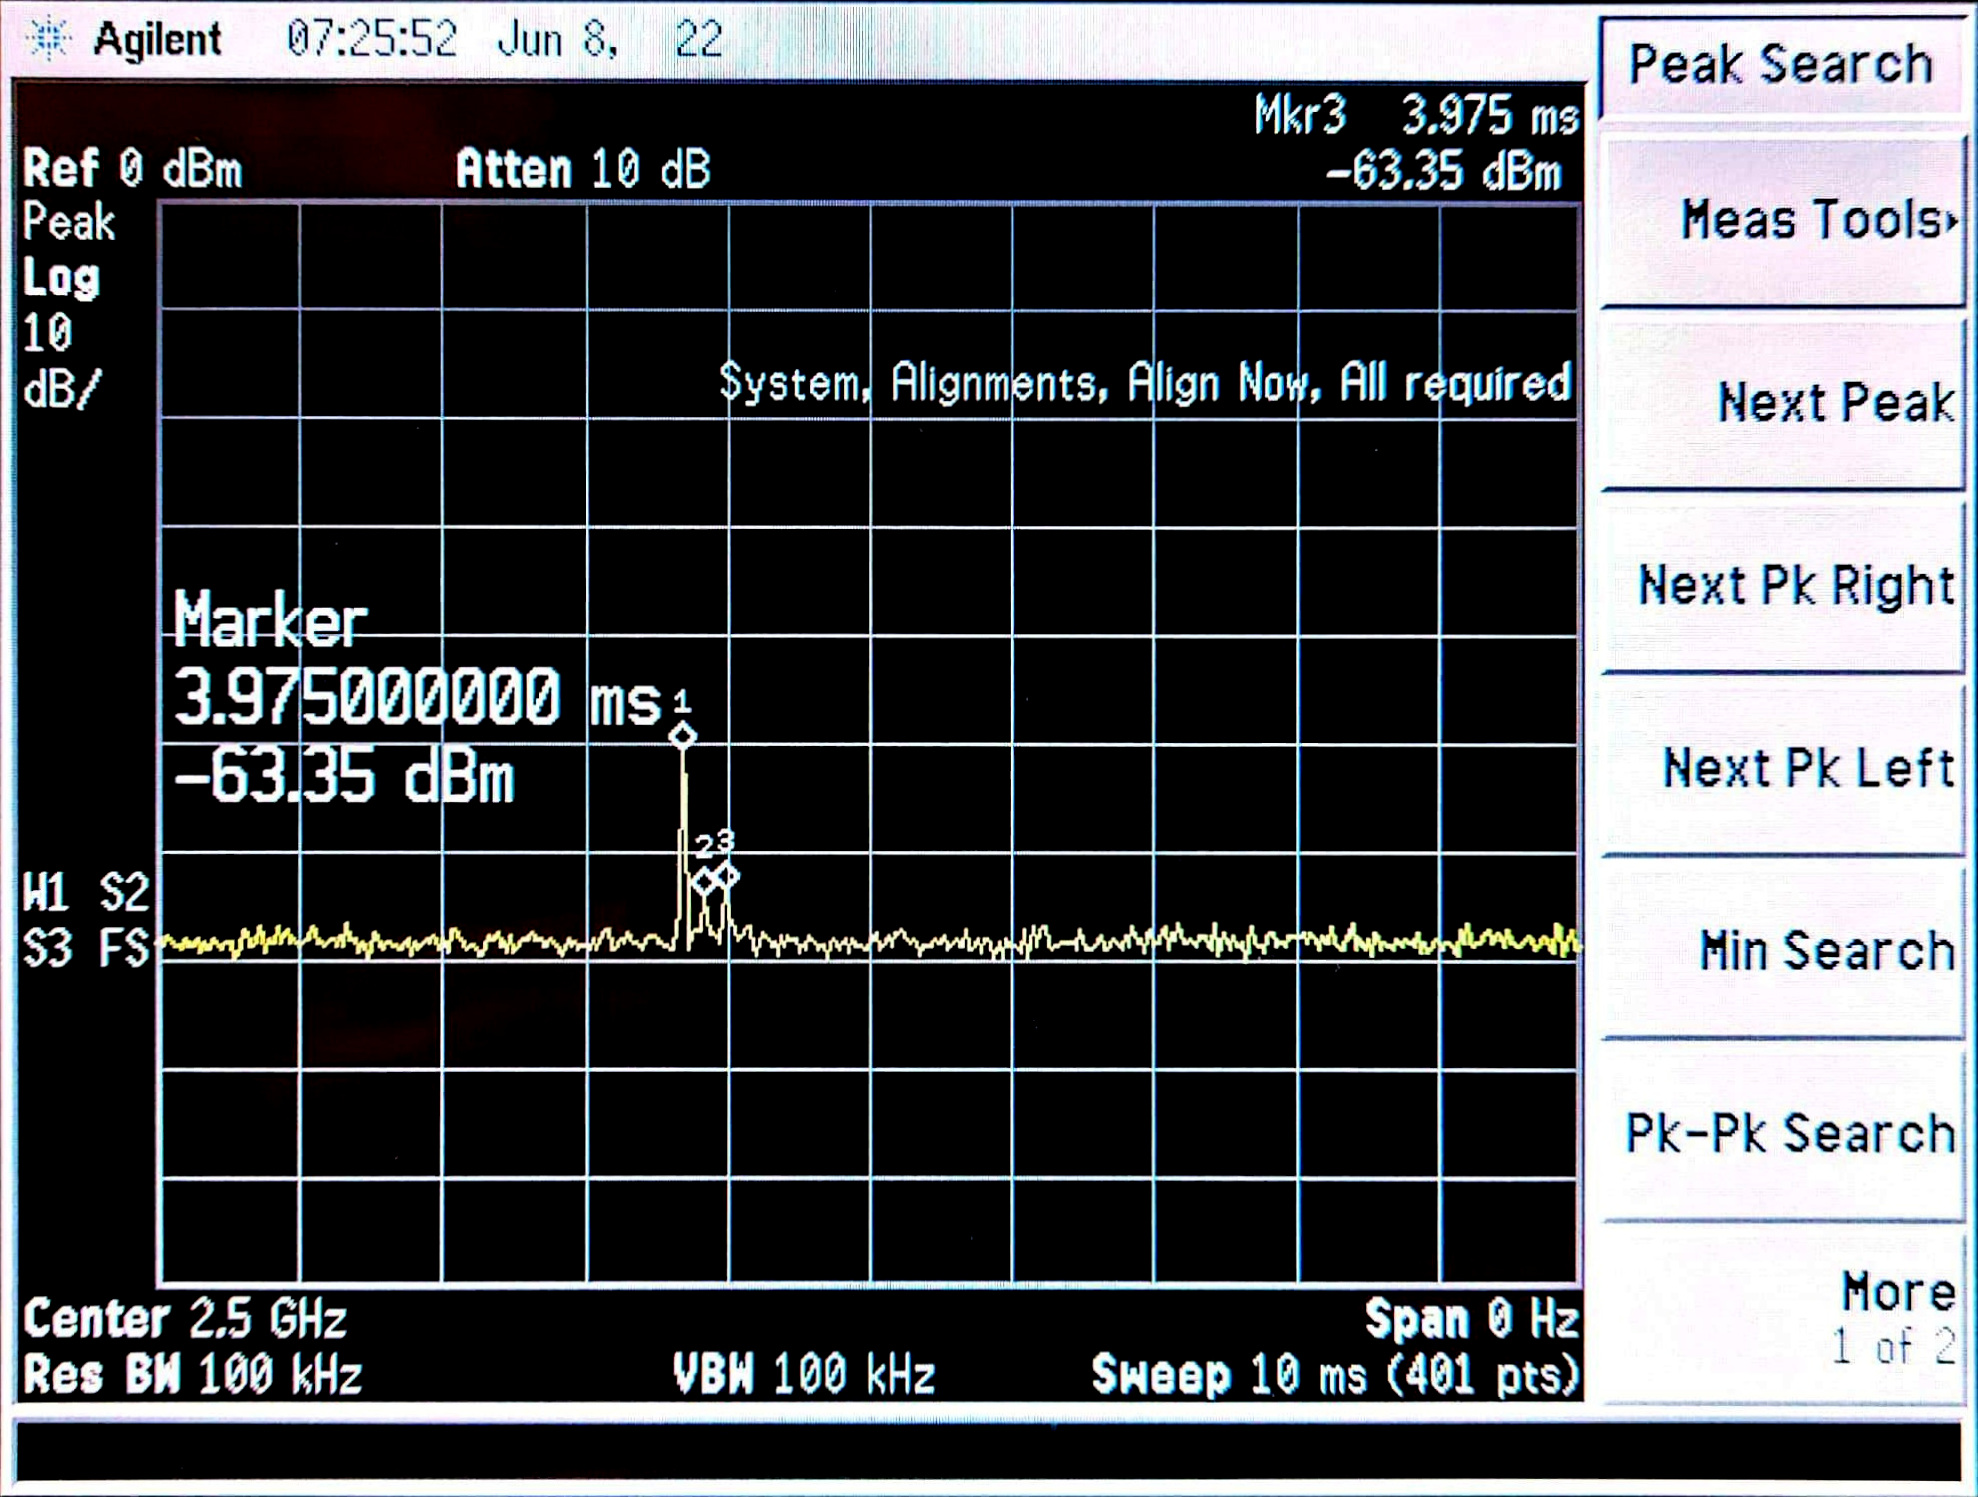
\includegraphics[width=0.9\linewidth]{backup_figs/PDP_Multiple.jpg}
        \end{minipage}
    \end{tabular}
    \caption{Clockwise from top-left: The output of the PN sequence generator for a clock input of \SI{400}{\mega\hertz} at $0$dBm (a); The signal observed at the input of the \SI{28}{\giga\hertz} up-converter in the transmitter circuit (b); The signal observed at the output of the \SI{28}{\giga\hertz} down-converter in the receiver circuit (c); A snapshot of the power delay profiles consisting of a dominant LoS component, observed at \SI{2.5}{\giga\hertz} swept at \SI{10}{\milli\second} (d); Similar power delay profile snapshots consisting of additional components (e) and (f).}
    \label{F3}
\end{figure*}

\noindent{\textbf{NSF POWDER Deployment}}: As described in Sec.~\ref{S2}, our measurement system assembly constitutes an autonomous beam-steering controller replicated at both the Tx and the Rx, their respective sounder circuits, and a centralized nerve center for aggregation (RPyC), synchronization (NTP), and coordination (Kafka-Zookeeper). On the NSF POWDER testbed, the nerve center is deployed on a high-availability cluster of four Dell R$740$ compute nodes at the Fort Douglas datacenter, with fault tolerance being a key feature to ensure storage redundancy for the recorded data. As depicted in Fig.~\ref{F2}(b), the Tx is mounted on a building rooftop; while, as shown in Fig.~\ref{F2}(c), the Rx is mounted on a van (or a push-cart) that is driven (or pushed) along unplanned routes onsite. Remote monitoring and troubleshooting is provided for validation of geo-positioning, alignment, and power-delay profile samples. The goal of this measurement campaign was to obtain a reasonably large dataset of site-specific measurements for evaluating the propagation characteristics of \SI{28}{\giga\hertz} signals in vehicular communication settings. Thus, our propagation modeling activities included V$2$I measurements under manual, semi-, and fully-autonomous alignment operations traversing nine routes spanning urban and suburban neighborhoods. Although our platform is capable of double-directional measurements and facilitates easy scalability to MIMO settings, in this campaign, we focus only on \emph{beam-steered measurements} for spatial consistency evaluations.

\noindent{\textbf{Post-Processing}}: Using GNURadio utilities, the metadata file corresponding to the route-specific power-delay profile records at the Rx is parsed to extract timestamp information, which is then associated with the geo-positioning and alignment logs at both the Tx and the Rx. The samples in each synchronized power-delay profile segment undergo pre-filtering via a low-pass filter (SciPy FIR implementation), time-windowing, and noise-elimination (via custom peak-search and thresholding heuristics). Coupled with transmission power and antenna gain values, the received power levels obtained from these processed samples allow the visualization of pathloss maps on the Google Maps API (rendered via the Bokeh toolbox), and the evaluation of pathloss behavior as a function of Tx-Rx distance, with validations against the $3$GPP TR$38.901$ and ITU-R M$.2135$ standards~\cite{MacCartneyModelsOverview}. The SAGE algorithm~\cite{SAGE} is used to extract multipath parameters, which facilitates RMS AoA direction spread studies~\cite{Indoor60G}. Under Tx-Rx distance and Tx-Rx alignment variations, we probe signal decoherence patterns via the spatial/angular autocorrelation coefficient~\cite{MacCartneySpatialStatistics}.
\vspace{-4mm}

% Numerical evaluations I: Pathloss studies and Spatial consistency evaluations
\section{Pathloss and Spatial Consistency Evaluations}\label{S4}
In this section, we outline the results of our evaluations on the collected dataset. First, in Fig.~\ref{F4}(a), we visualize the calibration curves, obtained according to the procedures outlined in Sec.~\ref{S3}, depicting the linear relationship between the power calculated (in dB) from USRP readings corresponding to the received power-delay profiles and the reference power levels (in dB). Also, obtained via empirical recordings of the WR-$28$ antenna's operational characteristics, Fig.~\ref{F4}(b) and Fig.~\ref{F4}(c) illustrate its $2$D radiation patterns along the azimuth and elevation directions, respectively: these enable us to compute the gains at specific locations along a route and at specific degrees of alignment, crucial for the analyses detailed next.
\begin{figure*} [t]
     \centering
     \begin{subfigure}{0.358\linewidth}
         \centering
         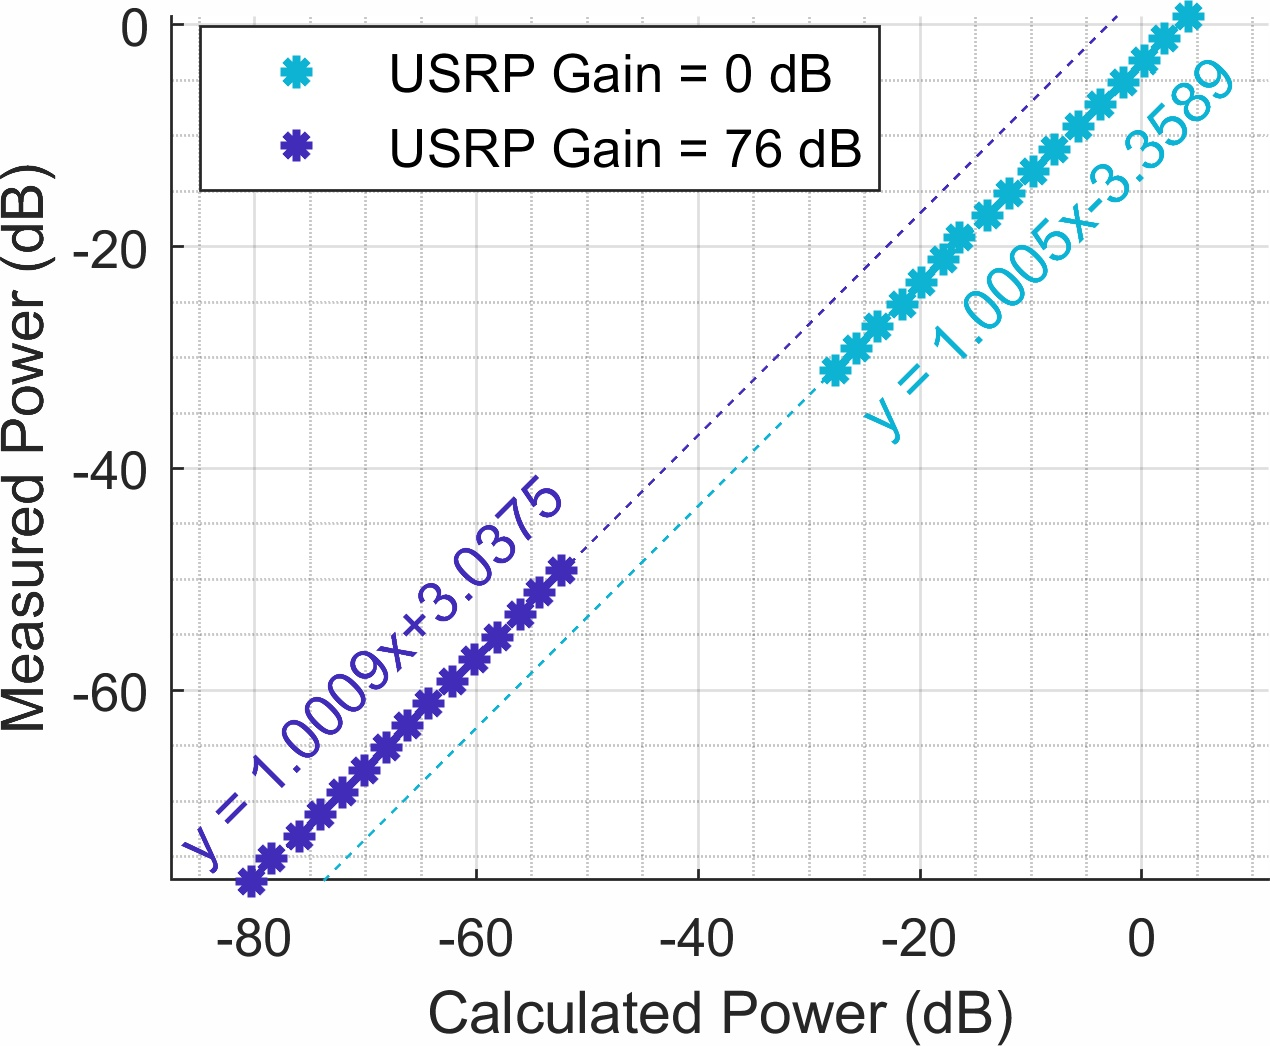
\includegraphics[width=1.0\linewidth]{figs/calibration.jpg}
         \caption{Calibration Curves}
         \label{F4a}
     \end{subfigure}
     \begin{subfigure}{0.31\linewidth}
         \centering
         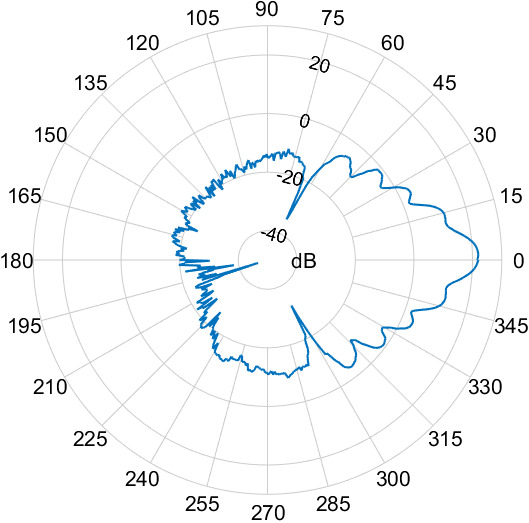
\includegraphics[width=1.0\linewidth]{figs/antenna_azimuth.jpg}
         \caption{Antenna Pattern (Azimuth)}
         \label{F4b}
     \end{subfigure}
     \begin{subfigure}{0.31\linewidth}
         \centering
         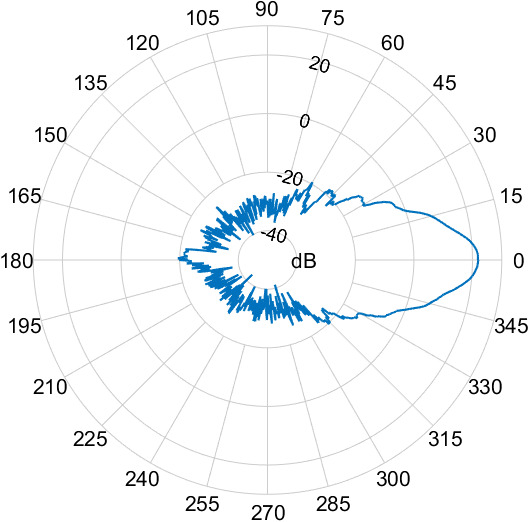
\includegraphics[width=1.0\linewidth]{figs/antenna_elevation.jpg}
         \caption{Antenna Pattern (Elevation)}
         \label{F4c}
     \end{subfigure}
     \caption{The calibration curves depicting measured power versus calculated power for USRP gains of \SI{0}{\deci\bel} and \SI{76}{\deci\bel} (a); and the normalized $2$D antenna patterns along the azimuth and elevation directions for the WR-$28$ horn antennas (b), (c).}
     \label{F4}
\end{figure*}

Fig.~\ref{F5} and Fig.~\ref{F6} depict the received power and pathloss heatmaps, superimposed on Google Hybrid maps of the routes traversed by the Rx onsite, with the Tx affixed on the rooftop of the William Browning building. Also, we compare the pathloss versus distance behavior of signals in our measurement campaign with large-scale urban macro-cellular pathloss standards ($3$GPP TR$38.901$ and ITU-R M$.2135$~\cite{MacCartneyModelsOverview}). These constitute both line-of-sight and non-line-of-sight models, with a Tx height of $h_{\text{Tx}}{\approx}$\SI{25}{\meter} and a Tx-Rx $2$D separation range of \SI{10}{\meter}${\leq}d_{2\text{D}}{\leq}$\SI{5000}{\meter}, which match the deployment specifications of our campaign, making them suitable candidates for empirical validations. As shown in Fig.~\ref{F7}(a), evaluating the pathlosses computed from our collected measurements against these standards for the urban campus (President's Circle), suburban neighborhood (S Walcott St), and urban vegetation (campus foliage) routes, we observe that while the $3$GPP and ITU-R standards model the empirical pathloss values for the urban campus route, they fail to accurately capture the pathloss vs distance behavior in suburban settings; additionally, these standards do not serve as good benchmarks for studying \SI{28}{\giga\hertz} propagation around foliage in urban environments.

Next, to analyze the multipath propagation characteristics of \SI{28}{\giga\hertz} signals, we use the SAGE algorithm~\cite{SAGE} to extract the complex attenuation ($\alpha$), delay ($\tau$), Doppler shift ($\nu$), and angles-of-arrival ($\phi,\theta$) of the $M$ specular paths arriving at the Rx while traversing a particular route onsite. Solving for the exact high-resolution maximum likelihood estimate of this parameter vector ($\bm{\xi}_{i}{=}[\alpha_{i},\tau_{i},\nu_{i},\phi_{i},\theta_{i}]^{\intercal},i{=}1,2,{\dots},M$) directly involves prohibitively large computation times~\cite{SAGE}. Thus, the SAGE algorithm solves for an approximate estimate of $\bm{\xi}_{i}$ via iterative executions of the E-step which computes the expectation of the log-likelihood given the observations and the previous estimate, and the M-step which computes the current estimate by maximizing over the E-step result. This iterative execution occurs until convergence, i.e., the change in parameter values across consecutive iterations is smaller than a predefined threshold. Using these estimates, in Fig.~\ref{F7}(b) we plot the RMS direction-spread ($\sigma_{\Omega}$) of the received signals while traversing the urban campus and urban vegetation routes: these spread metrics are computed employing the procedures outlined in~\cite{Indoor60G}. From the estimated AoA azimuth and elevation values, we observe that the multipath components arriving at the Rx along the urban campus route demonstrate a relatively larger spread than those along the urban vegetation route.
\begin{figure*} [t]
     \centering
     \begin{subfigure}{0.460\linewidth}
         \centering
         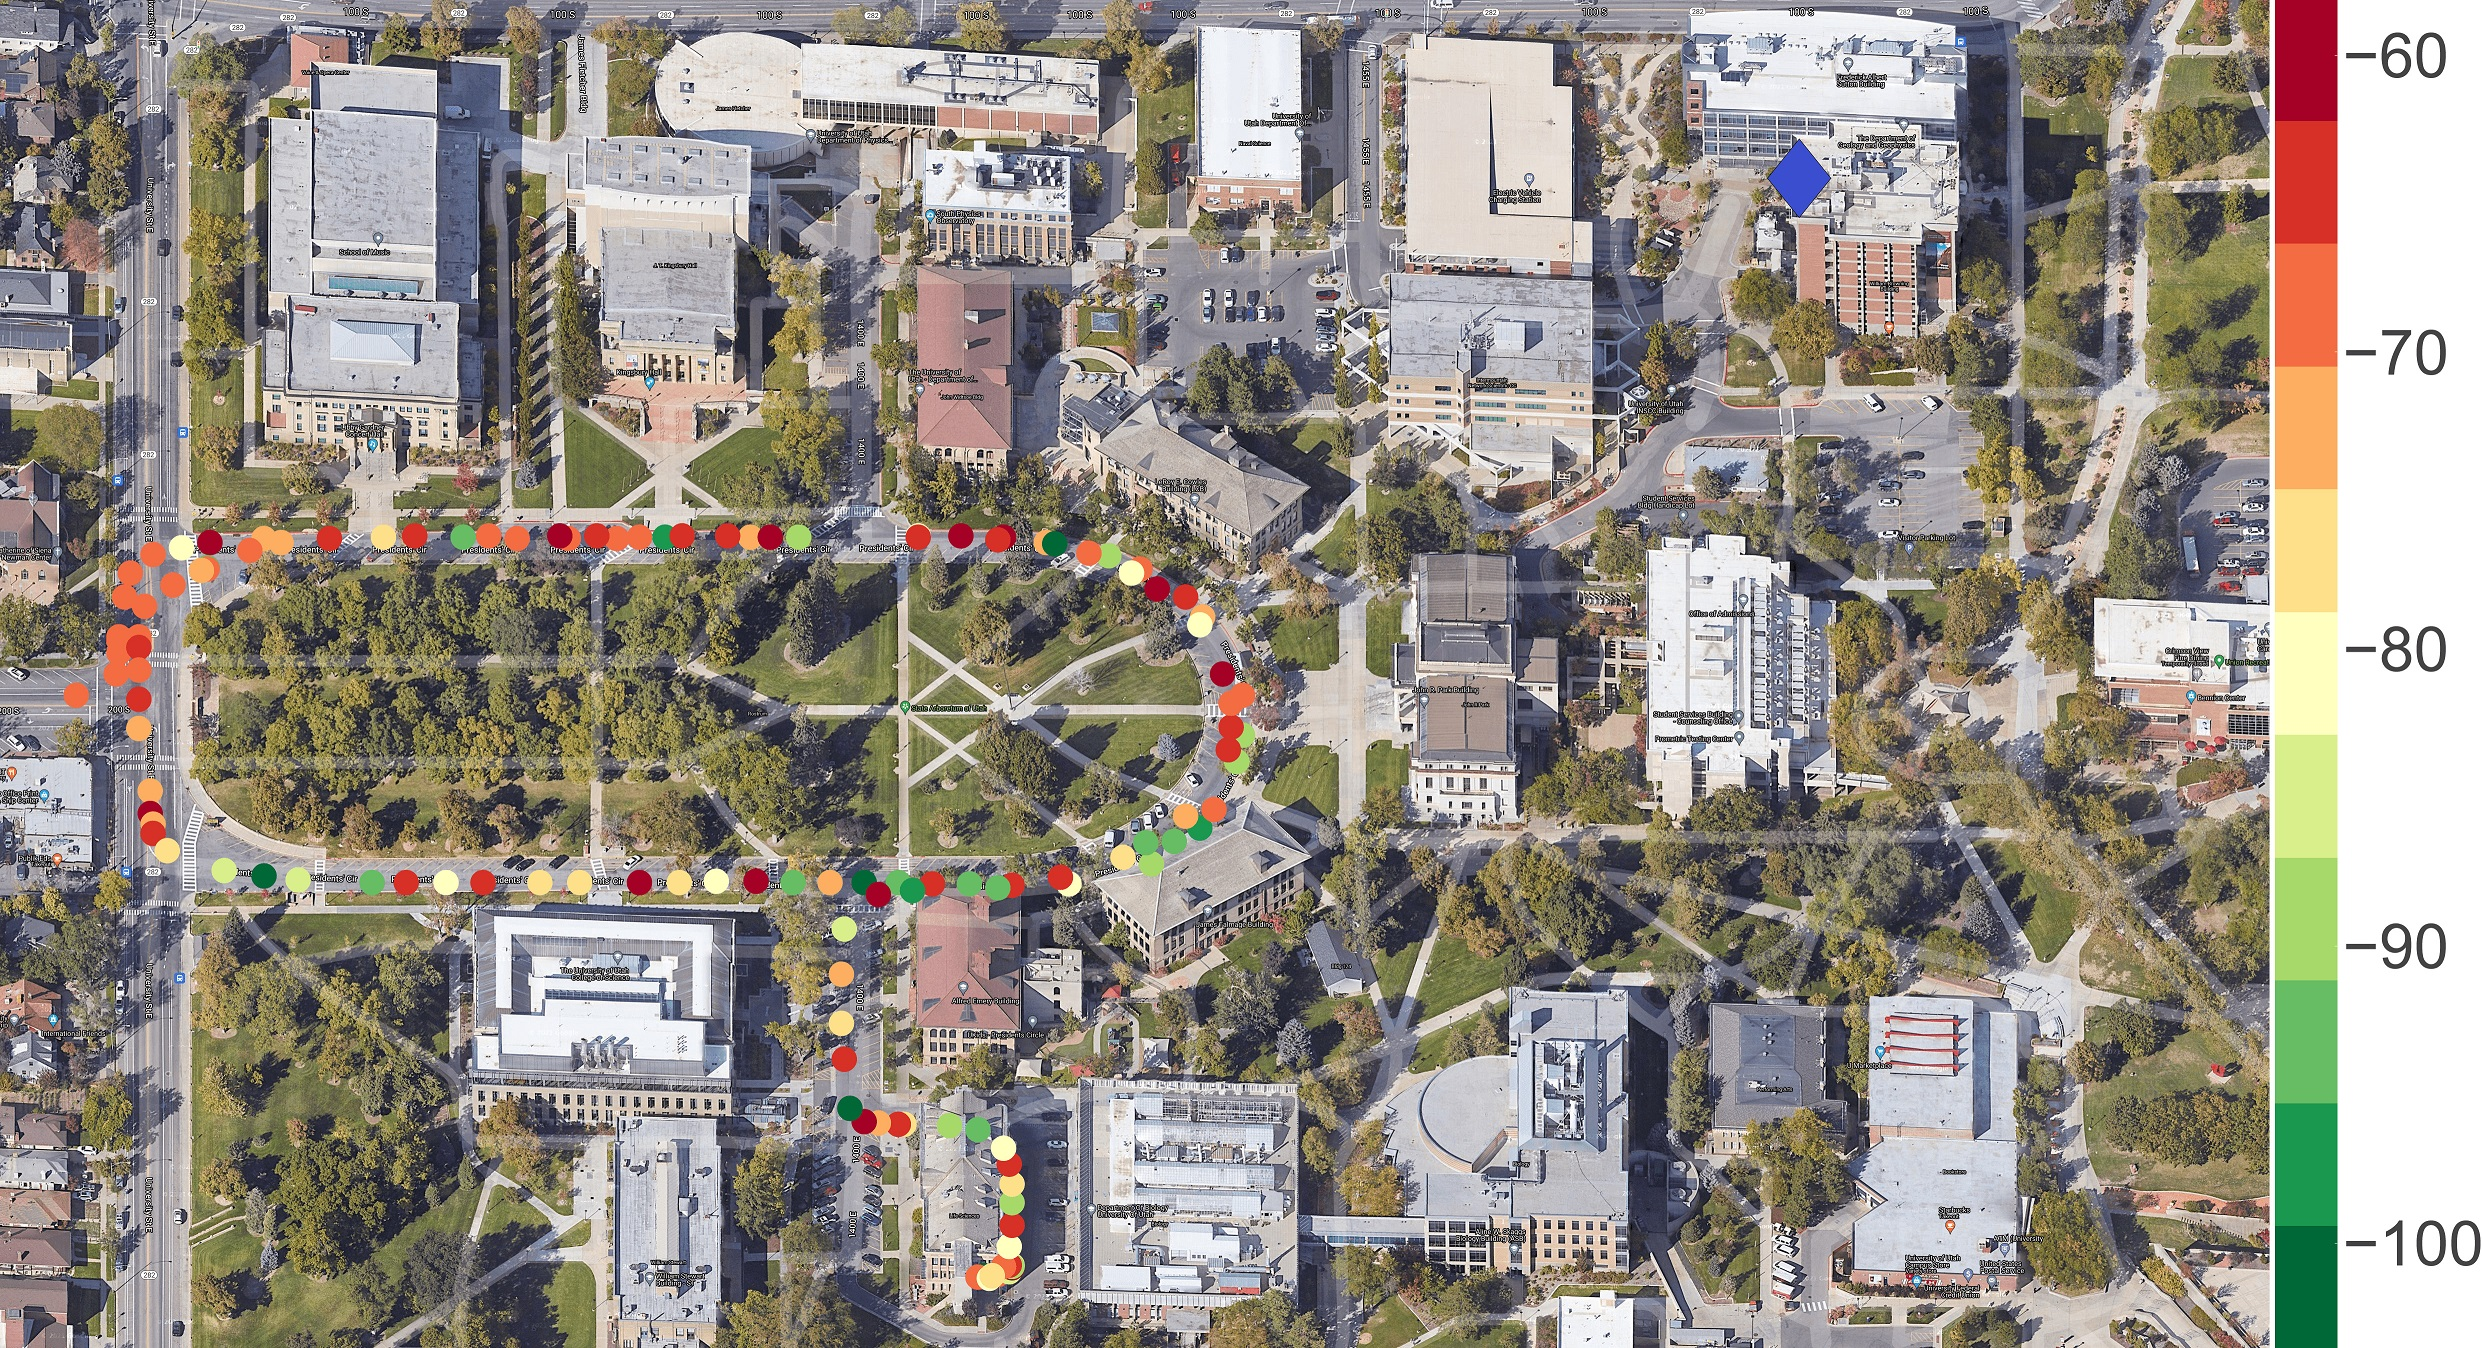
\includegraphics[width=1.0\linewidth]{figs/rx_urban_campus.jpg}
         \caption{Urban Campus (President's Circle)}
         \label{F5a}
     \end{subfigure}
     \begin{subfigure}{0.2579\linewidth}
         \centering
         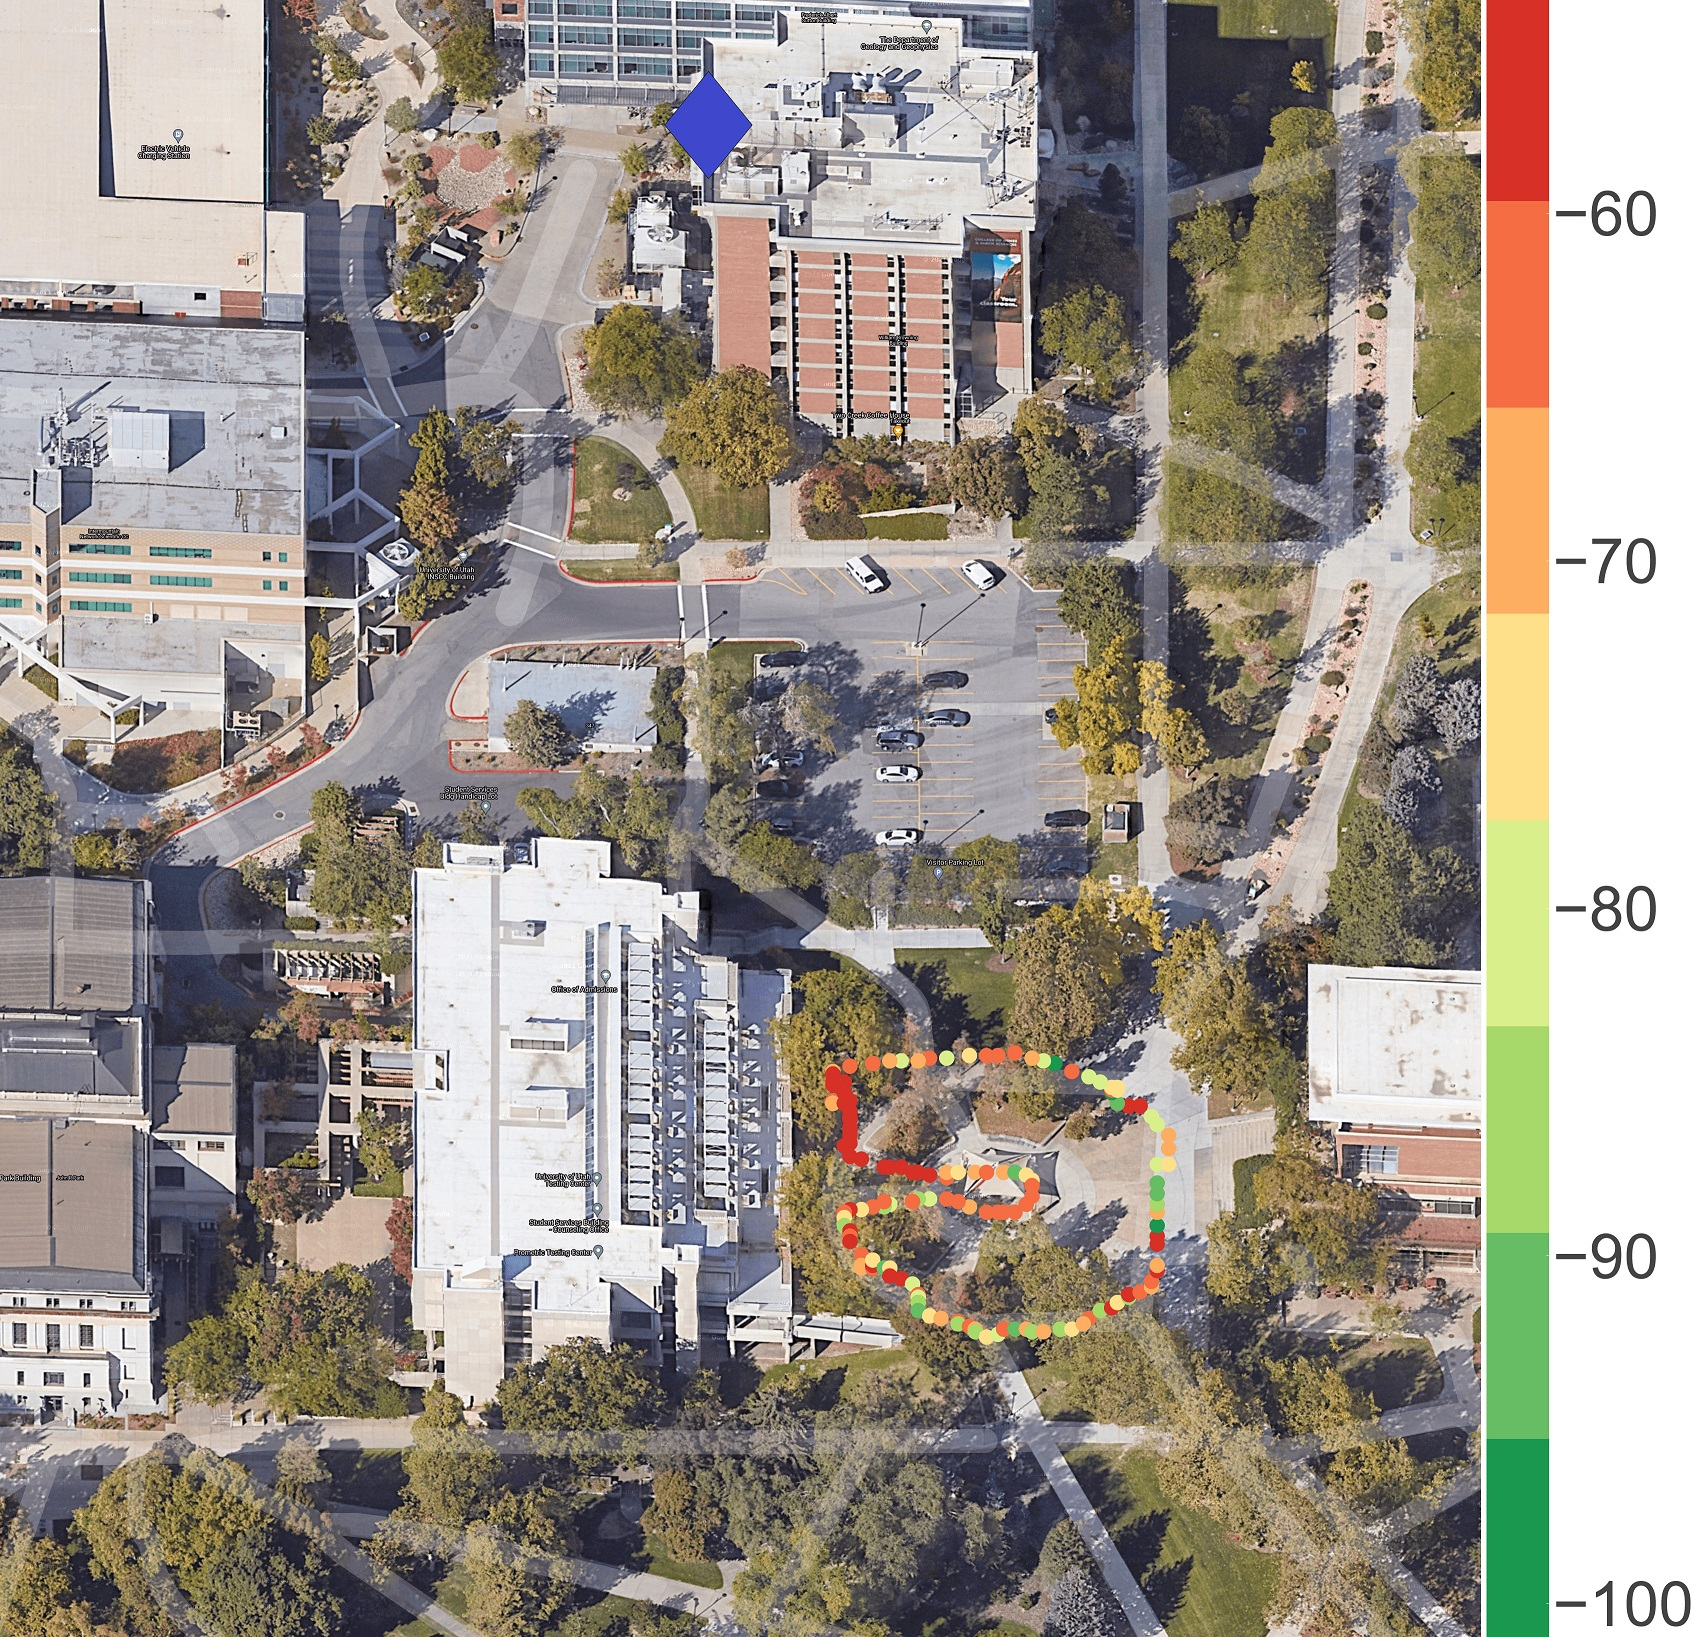
\includegraphics[width=1.0\linewidth]{figs/rx_urban_vegetation.jpg}
         \caption{Urban Vegetation}
         \label{F5b}
     \end{subfigure}
     \begin{subfigure}{0.2579\linewidth}
         \centering
         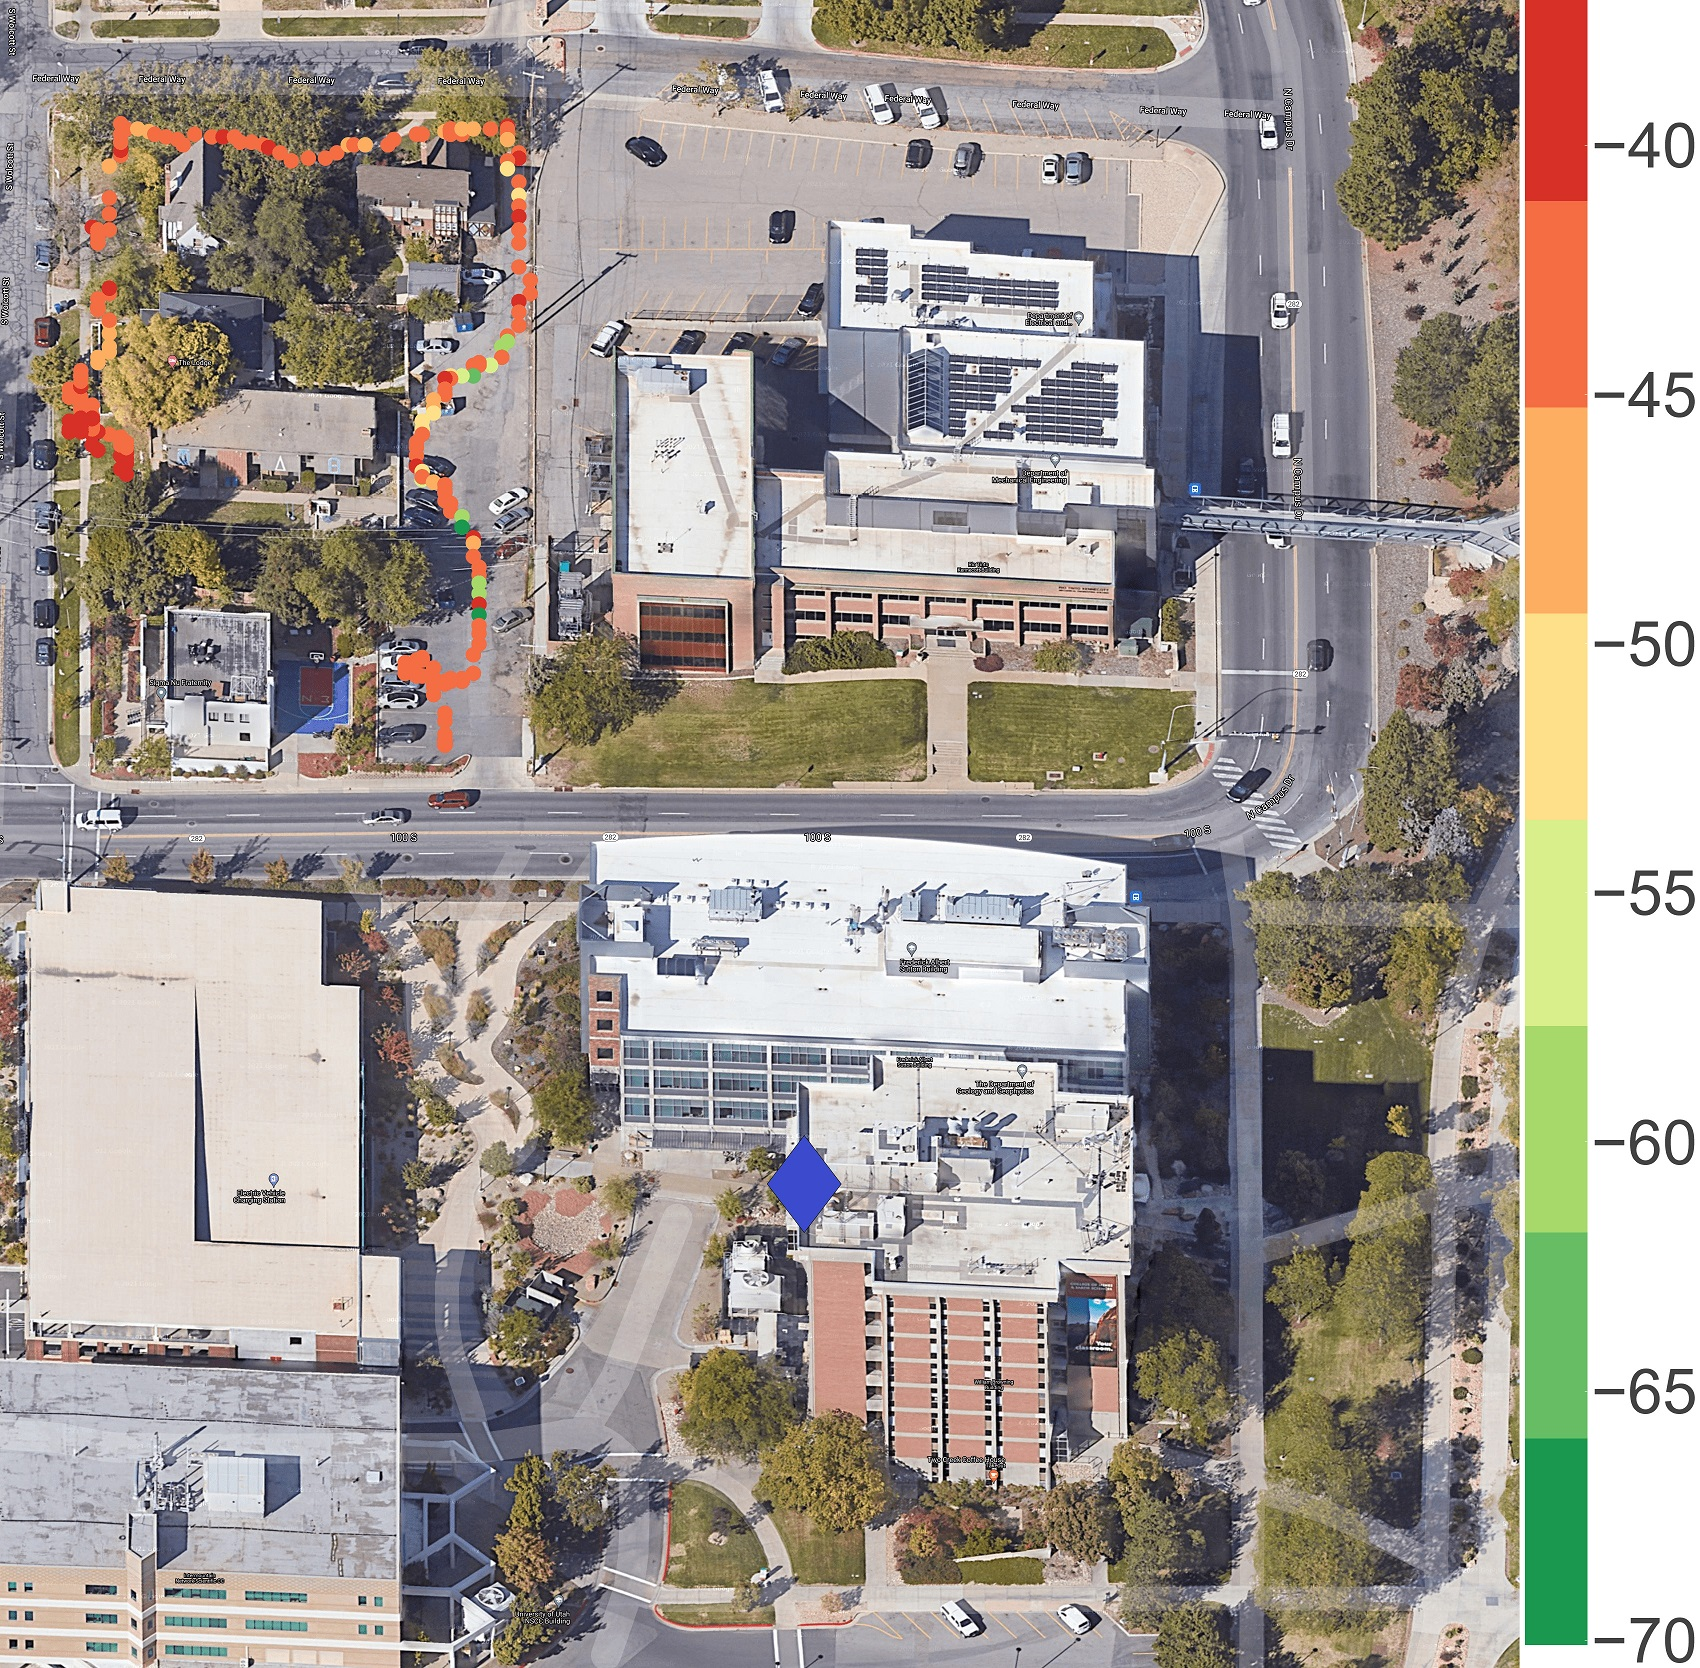
\includegraphics[width=1.0\linewidth]{figs/rx_suburban_fraternities.jpg}
         \caption{Suburban Neighborhood}
         \label{F5c}
     \end{subfigure}
     \vspace{-2mm}
     \caption{The received power values superimposed on a Google Hybrid map for urban campus (Rx on minivan), urban vegetation (Rx on cart), and suburban neighborhood (Rx on cart) routes, respectively. The heat-map color palette dots denote the Rx locations, while the purple diamond denotes the Tx location.}
     \label{F5}
\end{figure*}
\begin{figure*} [t]
     \centering
     \begin{subfigure}{0.48\linewidth}
         \centering
         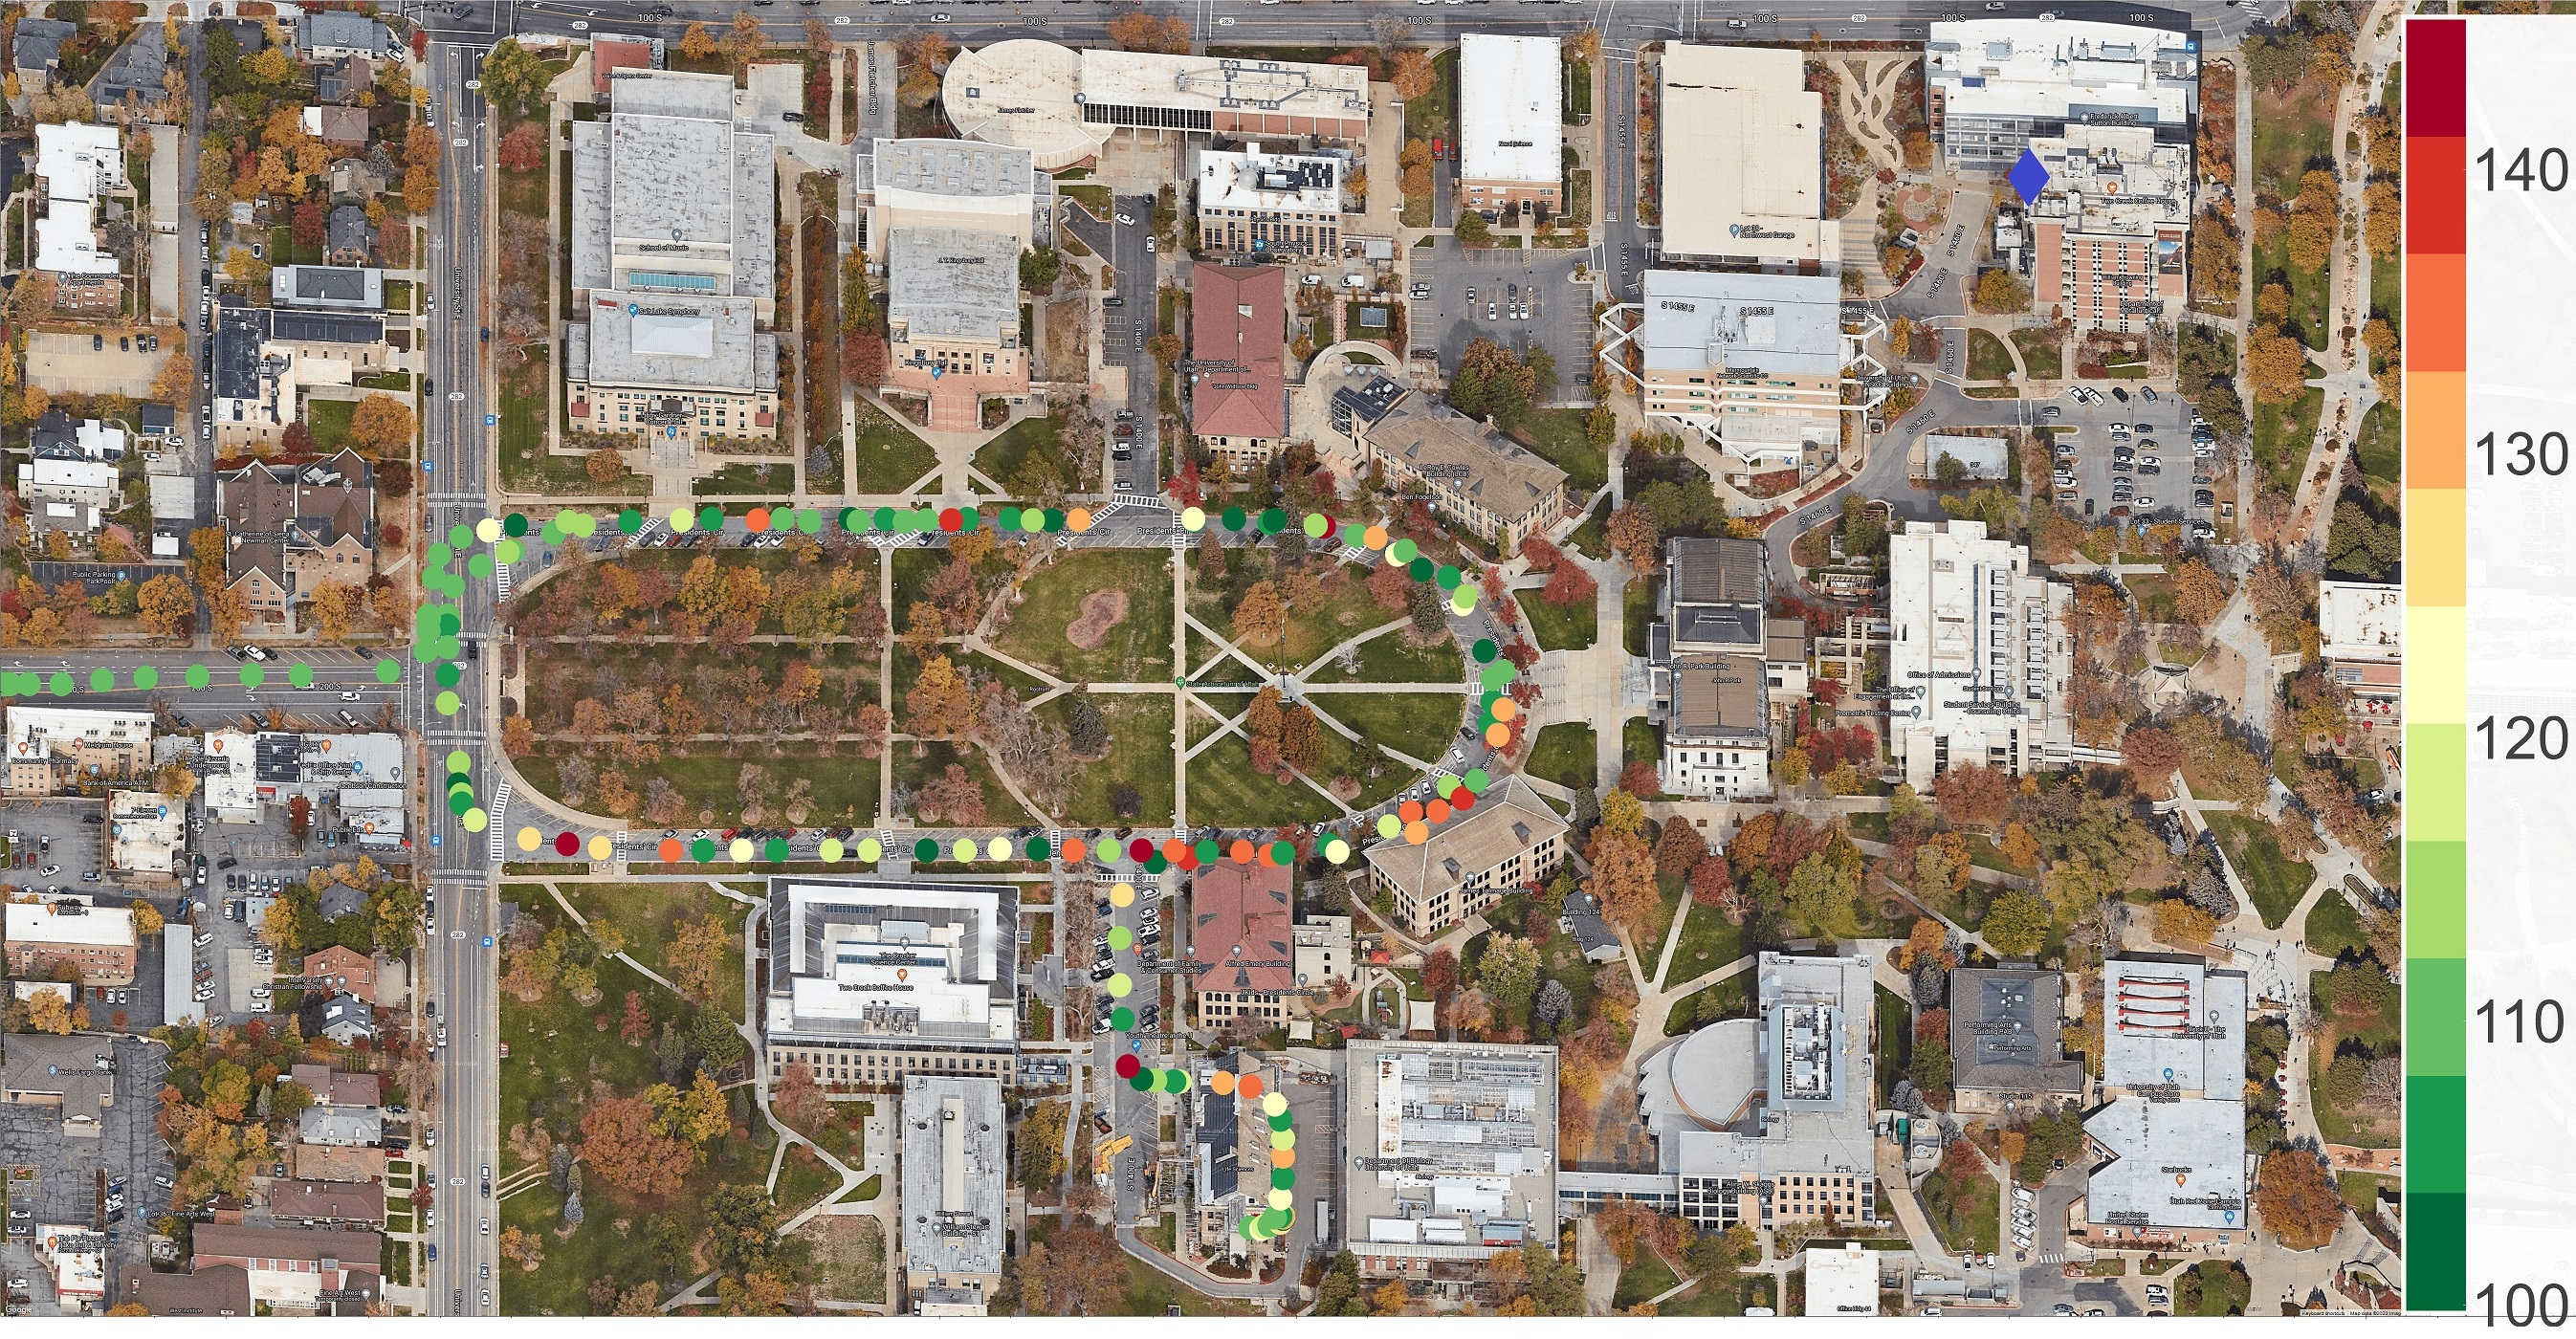
\includegraphics[width=1.0\linewidth]{figs/pl_urban_campus.jpg}
         \caption{Urban Campus (President's Circle)}
         \label{F6a}
     \end{subfigure}
     \begin{subfigure}{0.245\linewidth}
         \centering
         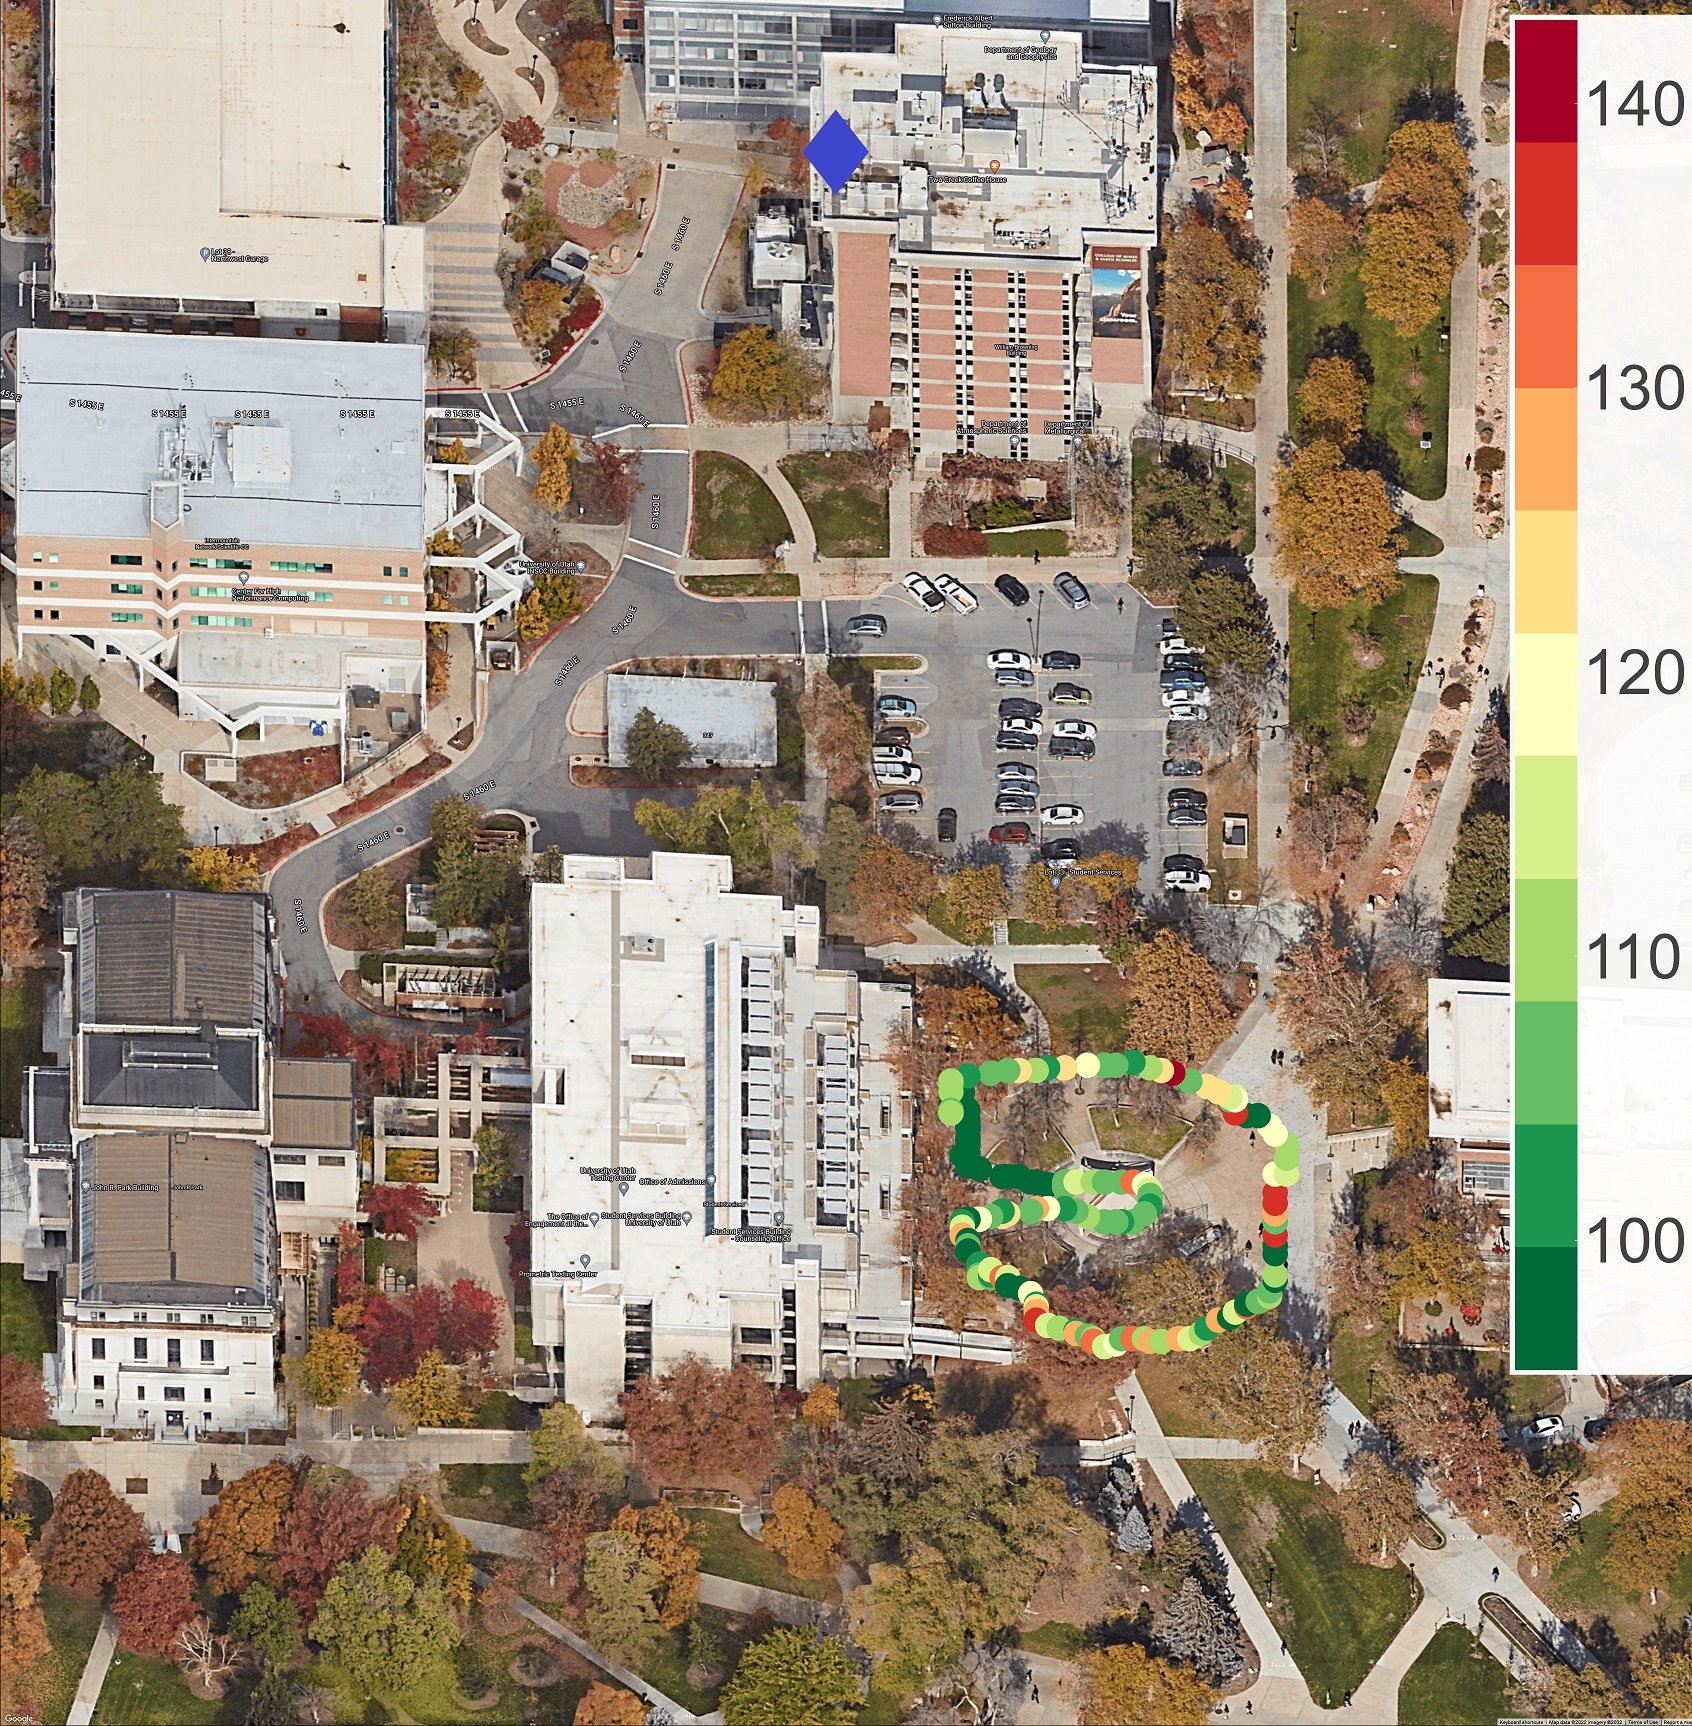
\includegraphics[width=1.0\linewidth]{figs/pl_urban_vegetation.jpg}
         \caption{Urban Vegetation}
         \label{F6b}
     \end{subfigure}
     \begin{subfigure}{0.245\linewidth}
         \centering
         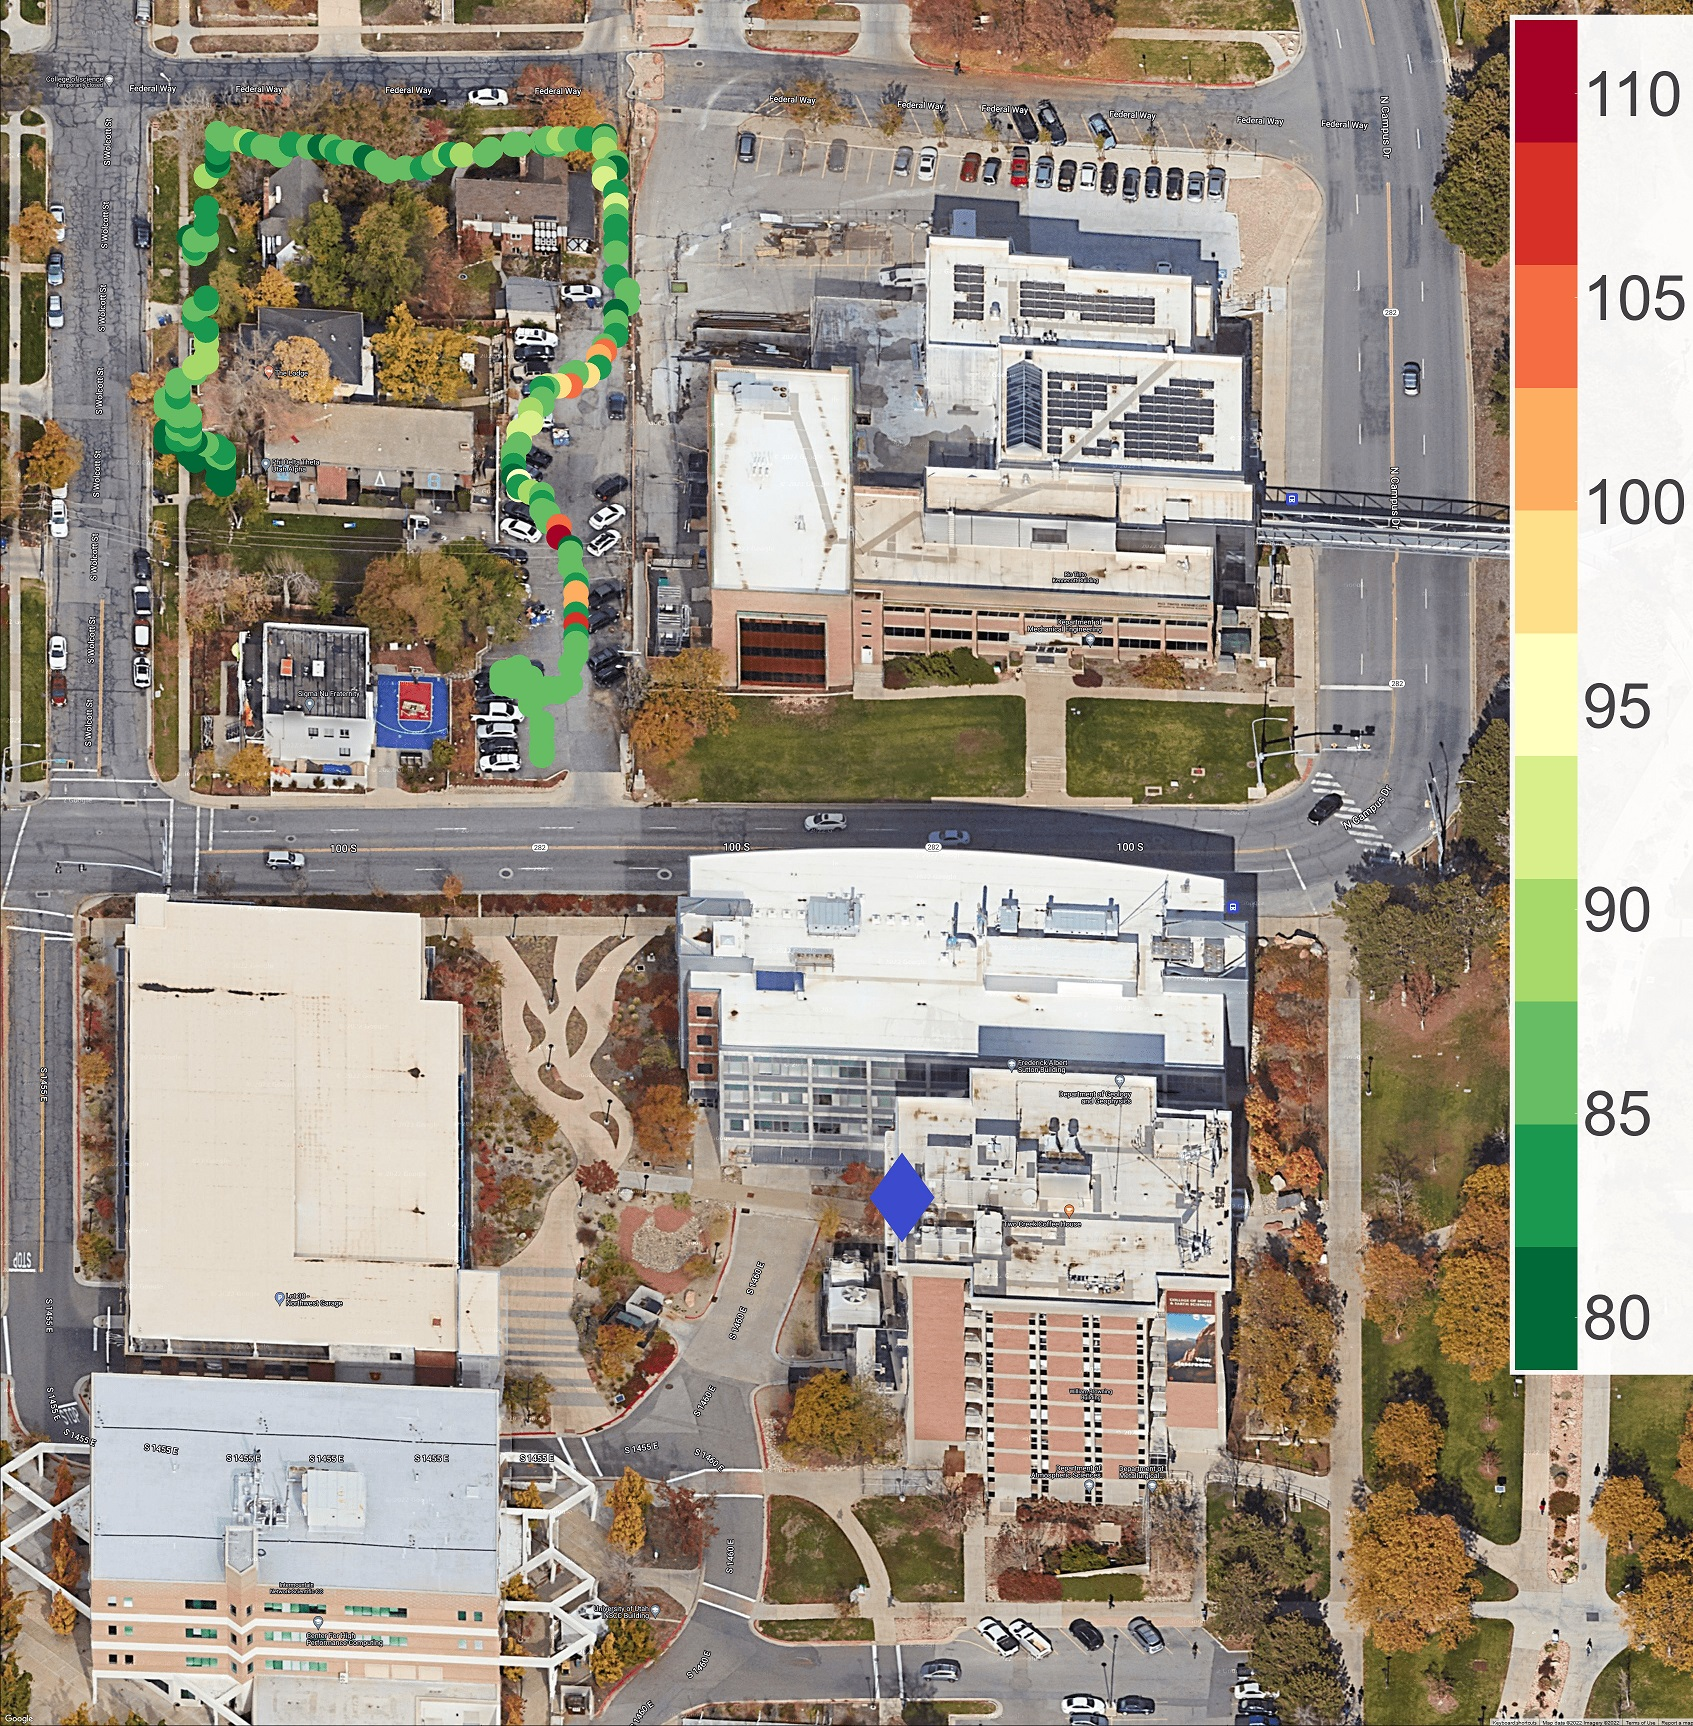
\includegraphics[width=1.0\linewidth]{figs/pl_suburban_fraternities.jpg}
         \caption{Suburban Neighborhood}
         \label{F6c}
     \end{subfigure}
     \vspace{-2mm}
     \caption{The pathloss values superimposed on a Google Hybrid map for urban campus (Rx on minivan), urban vegetation (Rx on cart), and suburban neighborhood (Rx on cart) routes, respectively. The heat-map color palette dots denote the Rx locations, while the purple diamond denotes the Tx location.}
     \label{F6}
\end{figure*}
\begin{figure*} [t]
     \centering
     \begin{subfigure}{0.485\linewidth}
         \centering
         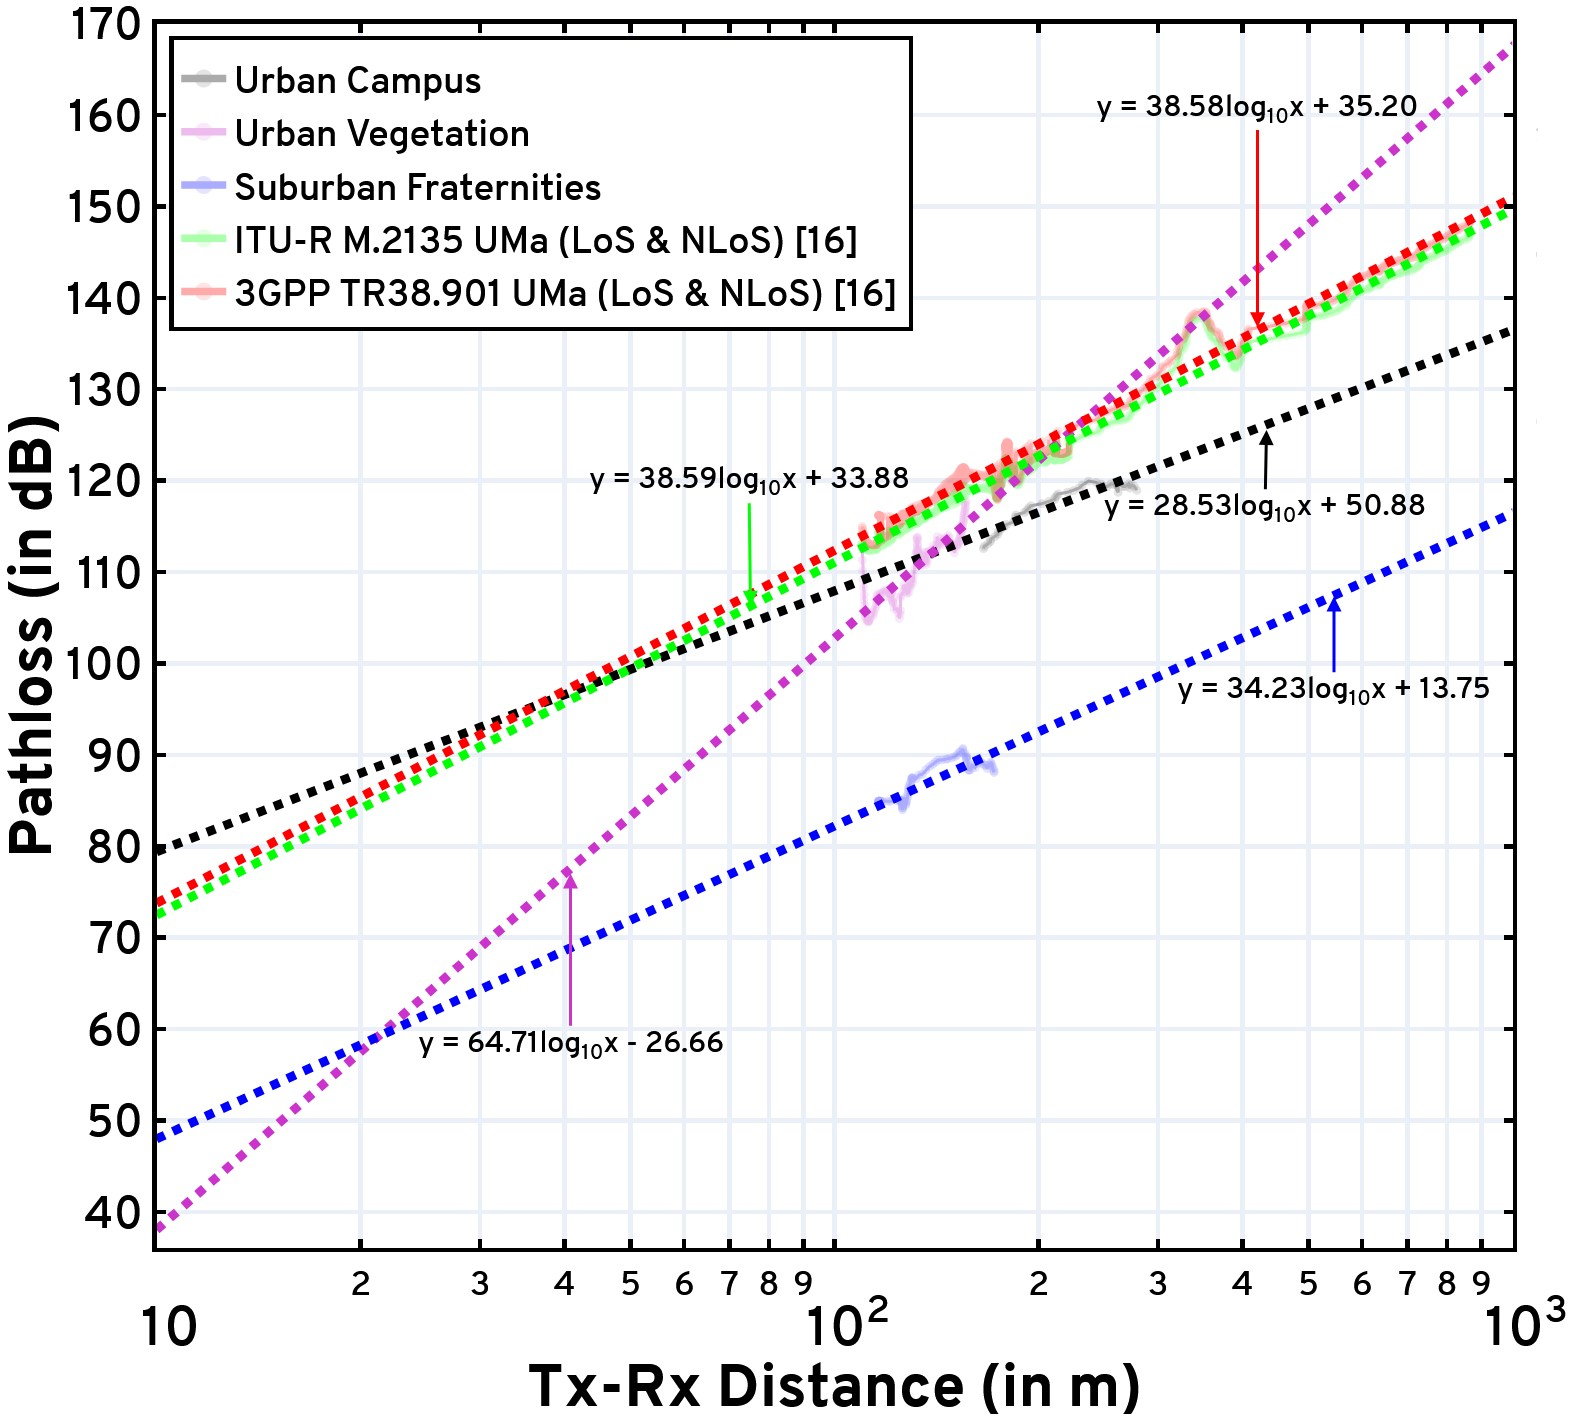
\includegraphics[width=1.0\linewidth]{figs/pl_distance_updated.jpg}
         \caption{Pathloss vs Tx-Rx Distance}
         \label{F7a}
     \end{subfigure}
     \begin{subfigure}{0.505\linewidth}
         \centering
         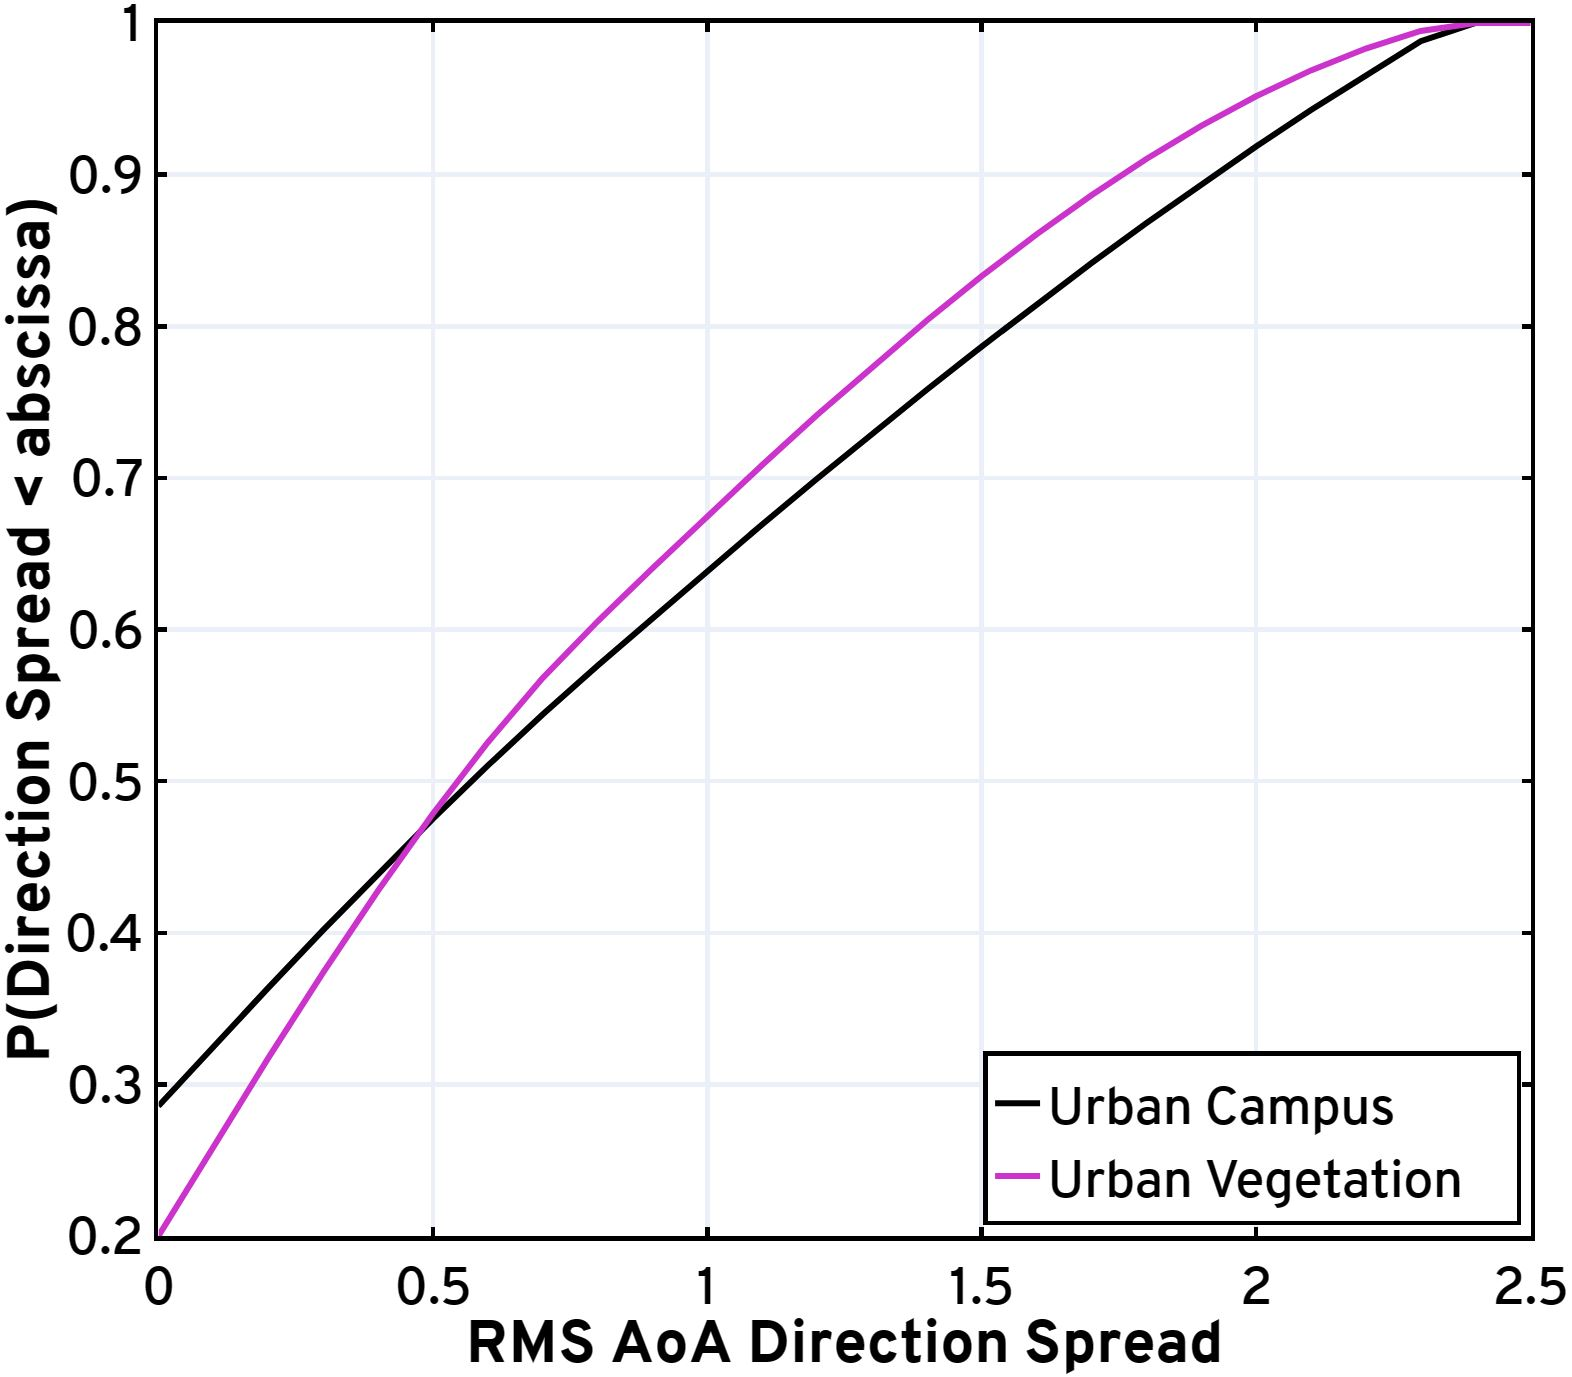
\includegraphics[width=1.0\linewidth]{figs/rms_direction_spread_updated.jpg}
         \caption{RMS AoA Direction Spread}
         \label{F7b}
     \end{subfigure}
     \vspace{-2mm}
     \caption{An illustration of the pathloss values computed from the various routes traversed during the measurement campaign compared against the $3$GPP TR$38.901$ and ITU-R M.$2135$ standards, with the dashed lines denoting the corresponding fitted models (a); and a plot depicting the cumulative distribution function of the RMS AoA direction-spread computed from the parameter estimates obtained via SAGE, for the urban-campus and urban-vegetation routes.}
     \label{F7}
\end{figure*}

Finally, to study the spatial decoherence behavior of \SI{28}{\giga\hertz} signals in V$2$X scenarios, we evaluate the spatial/angular autocorrelation coefficient along specific Rx routes under the effects of Tx-Rx distance and alignment: this coefficient is computed according to the steps laid down in~\cite{MacCartneySpatialStatistics}, wherein for each Rx location change, the amplitude term in~\cite{MacCartneySpatialStatistics} constitutes the magnitude of all the power-delay profile components (along the excess delay axis) in a recorded measurement at that location, with the expectation taken over the ensemble. Fig.~\ref{F8}(a) illustrates these spatial consistency plots vis-\`{a}-vis distance, under perfect Tx-Rx alignment conditions, wherein exponential functions are fit to the computed coefficient values for the urban campus, suburban neighborhood, and urban vegetation routes. We note decreasing correlation trends between the recorded power-delay profile samples under increasing Tx-Rx separation. Similarly, keeping the Tx-Rx separation constant, Fig.~\ref{F8}(b) depicts the variation of the angular autocorrelation coefficient under increasing levels of misalignment between the Tx and Rx antennas, while traversing the urban campus and suburban neighborhood routes. We observe rapid decorrelation across the evaluated samples even at small amounts of misalignment, highlighting the characteristics of our directional WR-$28$ horn antennas, and illustrating the need for accurate beam-steering in mmWave V$2$X networks. In Figs.~\ref{F8}(a), (b), the channel does not get fully decorrelated since, in our \emph{beam-steered measurements}, the LoS component remains significant.
\begin{figure*} [t]
     \centering
     \begin{subfigure}{0.497\linewidth}
         \centering
         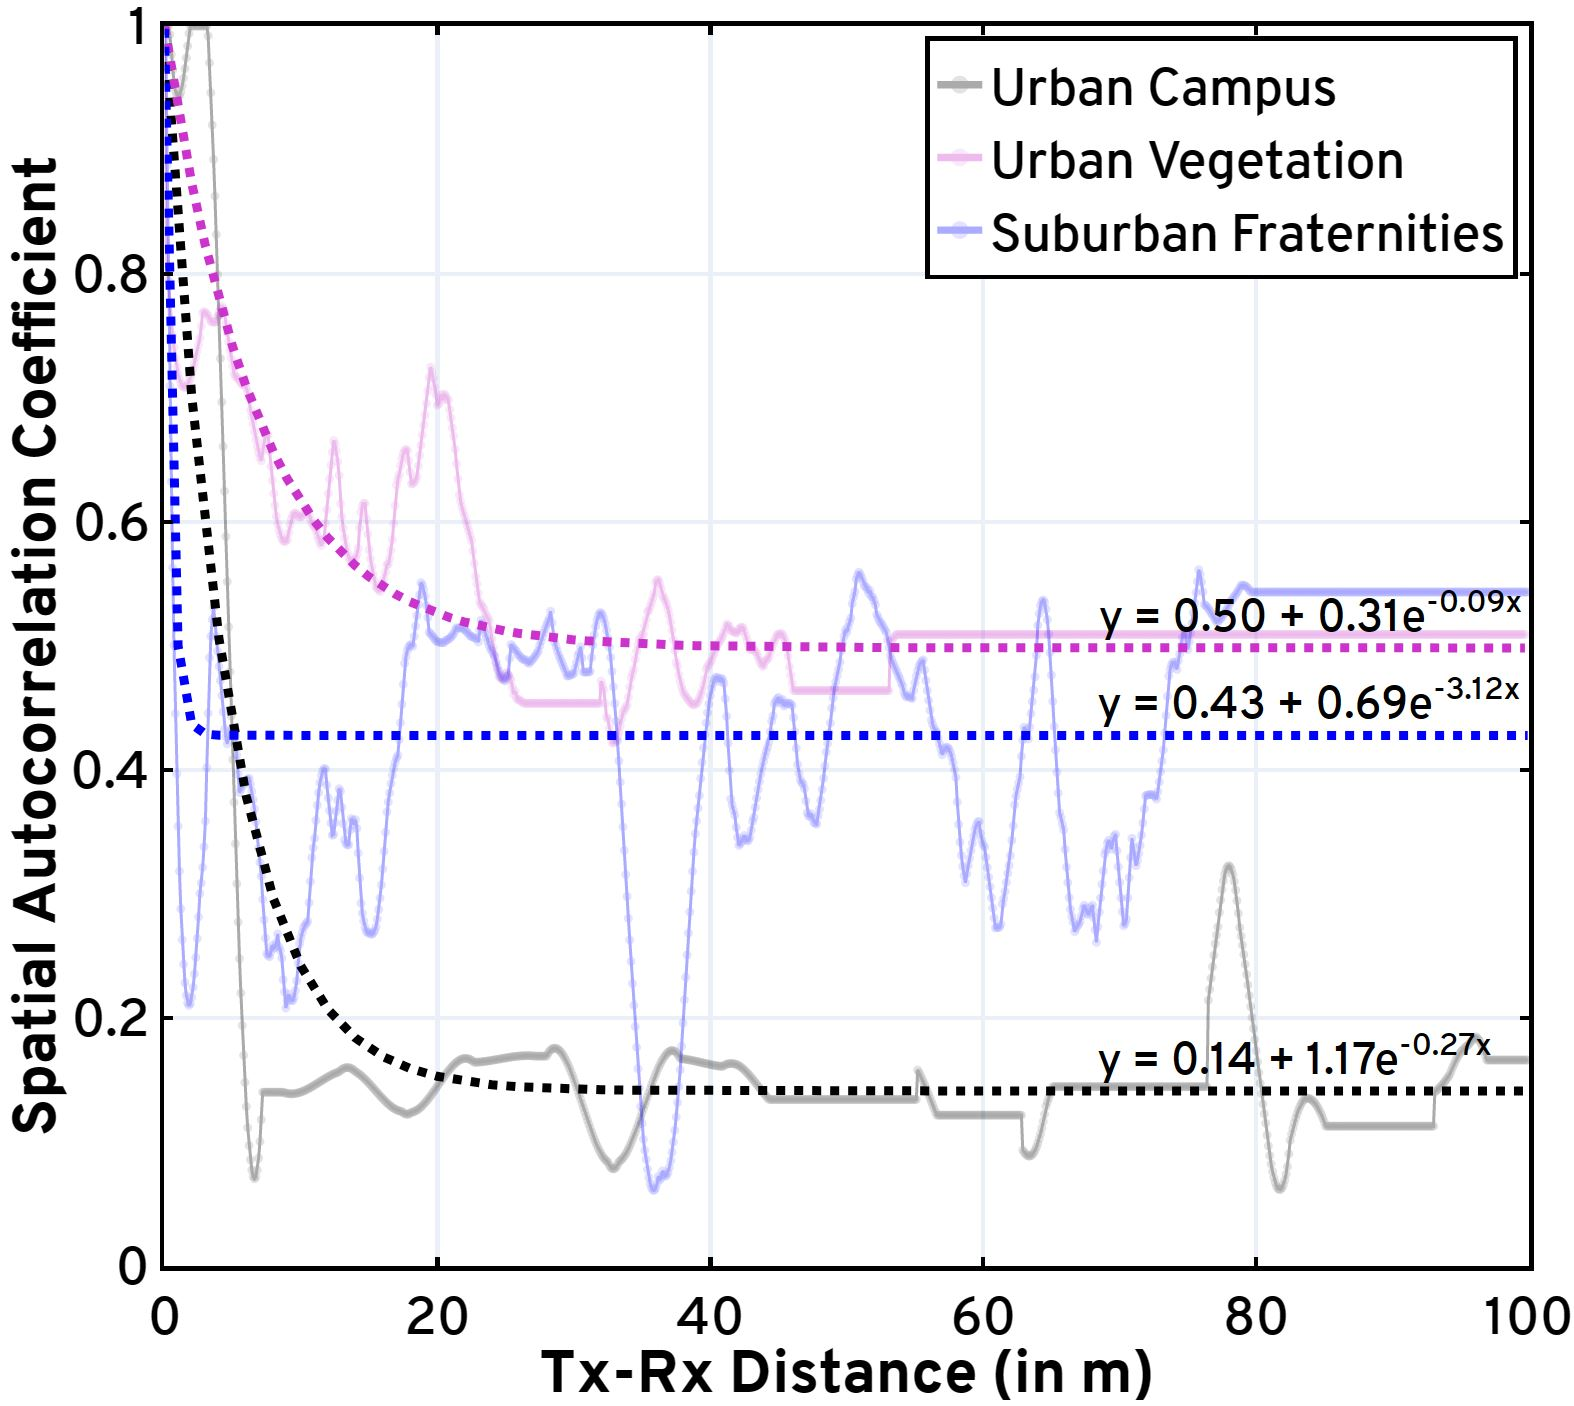
\includegraphics[width=1.0\linewidth]{figs/sc_distance_updated.jpg}
         \caption{Spatial Consistency vs Tx-Rx Distance}
         \label{F8a}
     \end{subfigure}
     \begin{subfigure}{0.493\linewidth}
         \centering
         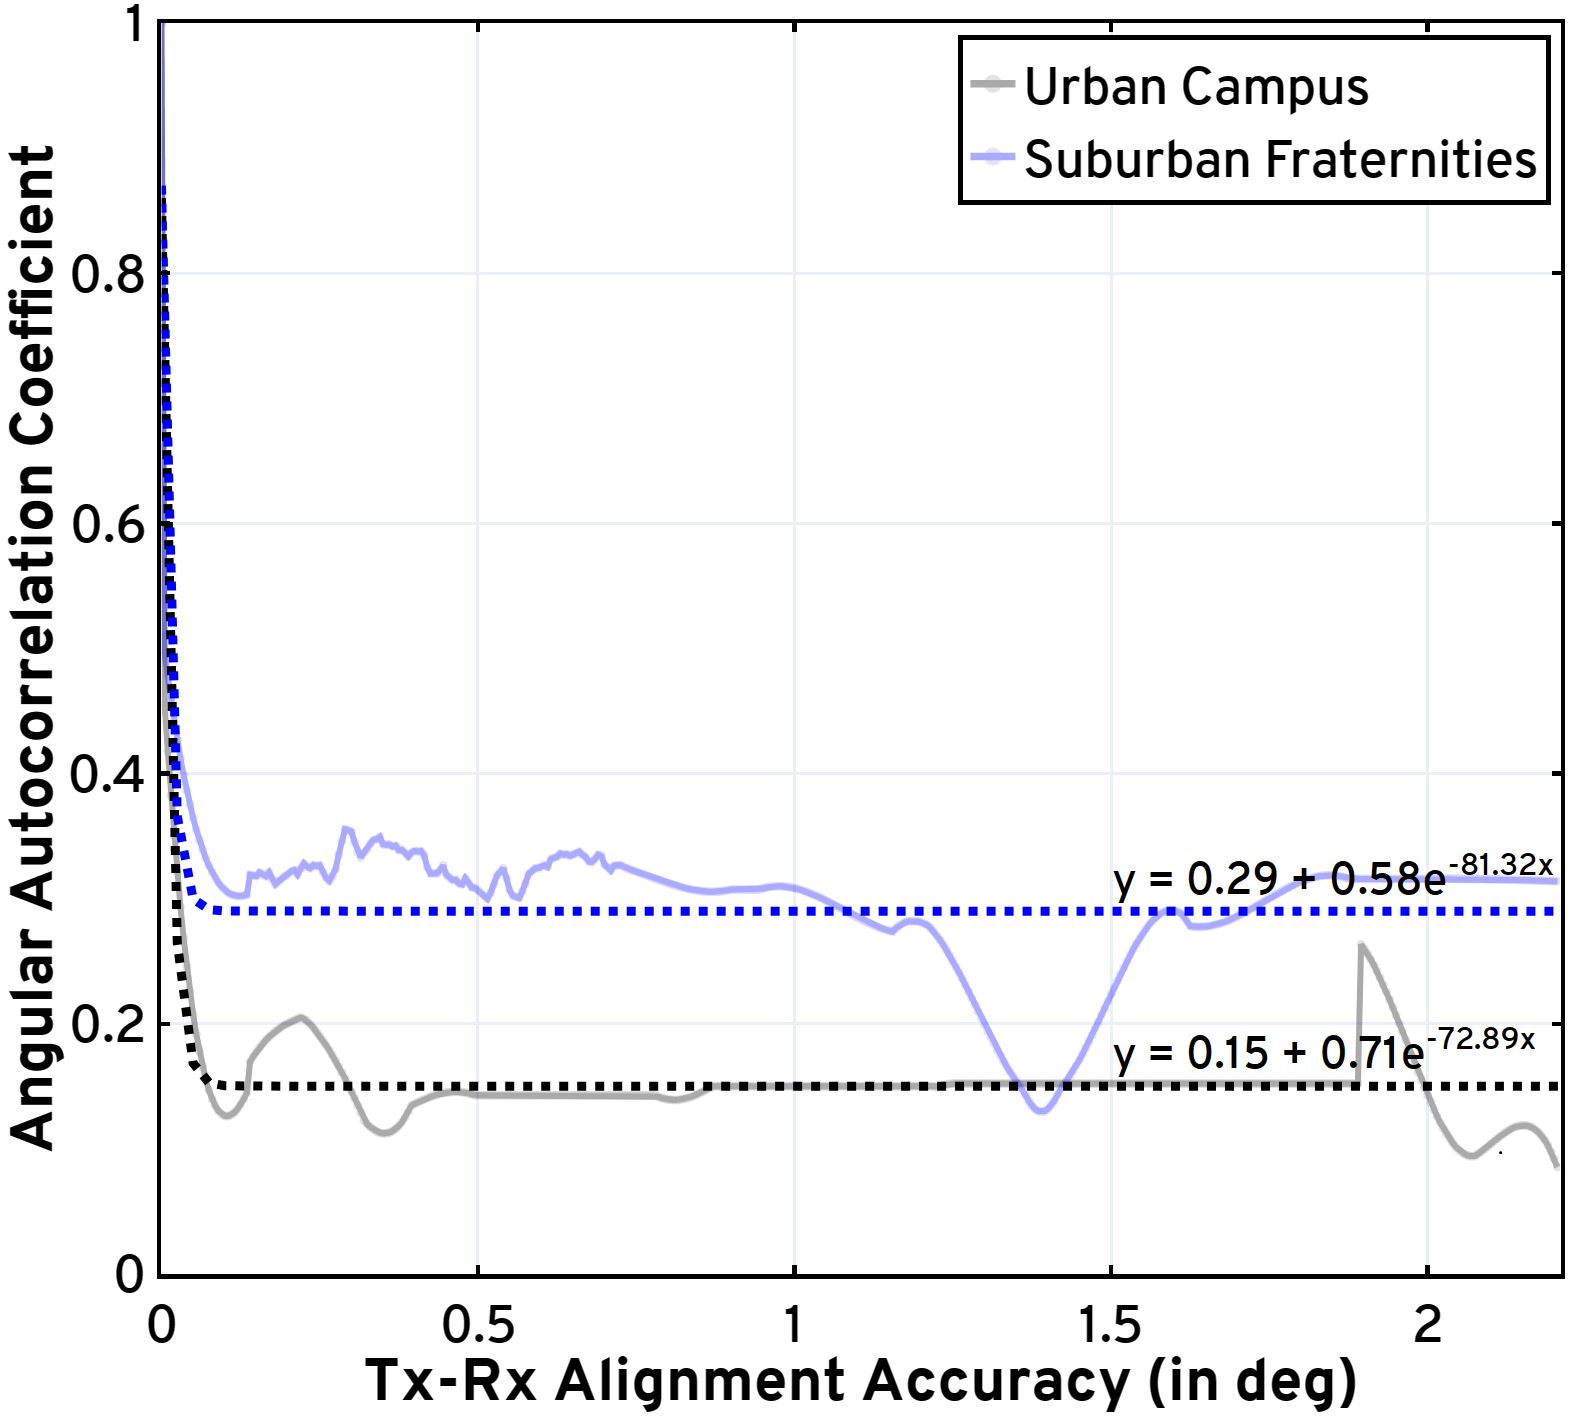
\includegraphics[width=1.0\linewidth]{figs/sc_alignment_updated.jpg}
         \caption{Spatial Consistency vs Tx-Rx Alignment Accuracy}
         \label{F8b}
     \end{subfigure}
     \vspace{-2mm}
     \caption{The plots depicting variations in the spatial/angular autocorrelation coefficient versus Tx-Rx distance (a) and Tx-Rx alignment accuracy (b).}
     \label{F8}
\end{figure*}
\vspace{-4mm}

% Numerical evaluations II: Multipath clustering and Channel model validations
\section{Multipath Clustering and Channel Modeling}\label{S5}
\vspace{-4mm}

% Concluding remarks and Future work
\section{Conclusion}\label{S6}
We discuss the design of a fully autonomous beam-steering platform coupled with a sliding correlator channel sounder, well-suited for mmWave V$2$X modeling. Corroborated onsite, this beam-steering system demonstrates superior performance vis-\`{a}-vis geo-positioning accuracy, alignment reliability, and tracking response times. Processing the power-delay profiles via custom noise elimination and thresholding heuristics, we perform pathloss evaluations against the $3$GPP TR$38.901$ and ITU-R M$.2135$ standards. Importantly, the continuous series of measurements facilitated by our design enables V$2$X spatial consistency studies vis-\`{a}-vis Tx-Rx distance and alignment.
\vspace{-4mm}

% References (main.bib)
\bibliographystyle{IEEEtran}
\bibliography{IEEEabrv,main} 

\end{document}
% Content ends